\documentclass[a4paper,10pt,titlepage]{report}
%%This template is based on Paco van Beckhoven's thesis.

\usepackage{xspace}
\usepackage{xargs}   % Use more than one optional parameter in a new commands
\usepackage{xcolor}

% Putting images next to each other
\usepackage[font=bf,]{caption}
\usepackage{subcaption}
\input{glyphtounicode}

% for last page
\usepackage{lastpage}

\usepackage[english]{babel}
\usepackage[utf8]{inputenc}
\usepackage{csquotes}
\usepackage[margin=1in]{geometry}
\usepackage{fancyhdr}
\usepackage{booktabs}
\usepackage{paralist}
\usepackage{graphicx}
\usepackage{tabularx}
\usepackage{adjustbox}
\usepackage{titlepic}
\usepackage{vhistory}
\usepackage{enumitem}
\usepackage{longtable}
\usepackage[backend=bibtex, style=ieee,citestyle=numeric-comp]{biblatex}
\usepackage[colorinlistoftodos, prependcaption]{todonotes}
\usepackage{placeins}
\usepackage{multirow}
\usepackage{amsmath,amssymb}
\usepackage[hidelinks]{hyperref}
\usepackage[acronym,nogroupskip,nohypertypes={acronym},toc,section=chapter]{glossaries}
\usepackage{amssymb}
\usepackage{verbatim}
\usepackage{cmap}
\usepackage{float}
\usepackage{hyperref}
\usepackage{wrapfig}
\usepackage{titlesec}

\newfloat{eqfloat}{h}{eqflts}
\floatname{eqfloat}{Equation}

\setcounter{secnumdepth}{4}


%\usepackage[ansinew]{inputenc}
%\usepackage[T1]{fontenc}
%\usepackage{libertine}
\input{glyphtounicode}

\pdfglyphtounicode{f_f}{FB00}
\pdfglyphtounicode{f_f_i}{FB03}
\pdfglyphtounicode{f_f_l}{FB04}
\pdfglyphtounicode{f_i}{FB01}

\pdfgentounicode=1



%Appendix package + appendix in chapter title
\usepackage[titletoc]{appendix}




%for highlighting findings
\usepackage{tcolorbox}

% for highlighting code examples
\usepackage{listings}

\newcommand{\ie}{\emph{i.e.},\xspace}
\newcommand{\eg}{\emph{e.g.},\xspace}
\newcommand{\etc}{\emph{etc.}\xspace}
\newcommand{\etal}{\emph{et al.}\xspace}

\newcommand{\sig}{\gls{sig}}
\newcommand{\sigs}{\glspl{sig}}

\newcommandx{\unsure}[2][1=]{\todo[linecolor=red,backgroundcolor=red!25,bordercolor=red,#1, inline]{#2}}
\newcommandx{\discussion}[2][1=]{\todo[linecolor=red,backgroundcolor=green!25,bordercolor=red,inline,#1]{#2}}

\newcommandx{\improvement}[2][1=]{\todo[linecolor=blue,backgroundcolor=blue!25,bordercolor=blue,#1]{#2}}

\newcommandx{\reminder}[2][1=]{\todo[linecolor=yellow,backgroundcolor=yellow!25,bordercolor=yellow,#1]{#2}}

\newcommandx{\lessprio}[2][1=]{\todo[linecolor=Plum,backgroundcolor=Plum!25,bordercolor=Plum,#1]{#2}}
\newcommandx{\todocontent}[2][1=]{\todo[author=\textbf{Planned content},backgroundcolor=Goldenrod!25,bordercolor=Goldenrod,inline,#1]{#2}}


%%Some additional table column specifiers, allowing for fixed width columns that wrap.
\newcolumntype{L}[1]{>{\raggedright\let\newline\\\arraybackslash\hspace{0pt}}p{#1}}
\newcolumntype{C}[1]{>{\centering\let\newline\\\arraybackslash\hspace{0pt}}p{#1}}
\newcolumntype{R}[1]{>{\raggedleft\let\newline\\\arraybackslash\hspace{0pt}}p{#1}}

\definecolor{ryel}{HTML}{fcd116}
\definecolor{rred}{HTML}{ce1126}
\definecolor{rblu}{HTML}{0a3eb9}
%these are examples of commands that may facilitate feedback annotations in the document
%replace \paco by your name and \ana by your supervisor's name
\newcommandx{\ana}[2][1=]{\todo[linecolor=rblu,backgroundcolor=ryel,bordercolor=rred,#1]{#2}}
\newcommandx{\simon}[2][1=]{\todo[author=Simon,linecolor=blue,backgroundcolor=white,bordercolor=red,#1]{#2}}


% -- title page is a modified version of https://github.com/software-engineering-amsterdam/latex/blob/master/thesis/uvamscse.cls
\newcommand{\email}[1]{\ttfamily\href{mailto:#1}{#1}}

\newcommand{\uvacoverfoot}{%
	\vfill
	\begin{center}
		\begin{tabular}{r|l}
			\multirow{3}{*}{
\includegraphics[height=48pt]{uva.pdf}}
			&\textsc{\Large University of Amsterdam}\\
			&\textsc{Faculty of Physics, Mathematics and Informatics}\\
			&\textsc{Master Software Engineering}\\
			&\url{http://www.software-engineering-amsterdam.nl}
		\end{tabular}
	\end{center}
}

\renewcommand{\maketitle}{%
	% The cover page
	% --------------
	\thispagestyle{empty}
	\enlargethispage{30pt}
	\renewcommand{\thefootnote}{\fnsymbol{footnote}}
	% Will be page 0, s.t. contents start on page 1
	\setcounter{page}{0}
	% \eccoverhead
	% Volume and article title, author(s)
	\vspace{60pt}
	\begin{center}
		{\Huge\bfseries Towards Automated Refactoring of Code Clones in Object-Oriented Programming Languages \par}
		% Earlier versions:
		% Assessing Test Suite Effectiveness Using Static Analysis
		% Predicting Test Suite Effectiveness Using Static Analysis
		% Predicting Test Suite Effectiveness Using Static Source Code Analysis
		% Assessing Test Suite Effectiveness Using Static Analysis
		% Predicting test suite effectiveness using static analysis
		\vspace{44pt}
		{\Large\bfseries Simon Baars \par}
		\email{simon.mailadres@gmail.com}\\
		\vspace{11pt}
		30 June 2019, \pageref{LastPage} pages
	\end{center}
	\vfill
	\begin{tabular}{ll}
		\textbf{Research supervisor:} Dr. Ana Oprescu, \email{ana.oprescu@uva.nl} \\
		\textbf{Host/Daily supervisor:} Xander Schrijen, \email{x.schrijen@sig.eu}\\
		\textbf{Host organisation/Research group:} Software Improvement Group (SIG), \url{http://sig.eu/}
	\end{tabular}
	\uvacoverfoot
	\newpage
	\setcounter{footnote}{0}
	\renewcommand{\thefootnote}{\arabic{footnote}}
	\setlength{\parskip}{0pt}
}

%\newcommand{\uvaabstract}{}latex
%\renewcommand{\abstract}[2][Abstract]{\renewcommand{\uvaabstract}{\chapter*{Abstract}%
%\par#2\newpage}}


%-------- End of ``title page''

%Fancy page headers
\pagestyle{fancy}
\fancyhf{}
\fancyhead[L]{\leftmark}
\fancyfoot[C]{\thepage}
\setlength{\headheight}{14pt}


%%FINDING ENV
\newcounter{findingctr}

\newenvironment{finding}{%      define a custom environment
	\refstepcounter{findingctr}% increment the environment's counter
	\begin{tcolorbox}
	\textbf{Finding \thefindingctr:}
}{\end{tcolorbox}}
% If you want numbers that start with the chapter or section number (e.g. 7.1.1 or 7.1) enable the following lines
%\usepackage{amsmath}
%\numberwithin{findingctr}{chapter}


% Decrease the size of all these lists
\setlist{noitemsep,topsep=4pt,parsep=1pt,partopsep=4pt}


\lstset{
	basicstyle=\footnotesize,        % the size of the fonts that are used for the code
	breakatwhitespace=false,         % sets if automatic breaks should only happen at whitespace
	breaklines=true,                 % sets automatic line breaking
	captionpos=b,                    % sets the caption-position to bottom
	frame=single,                    % adds a frame around the code
	language=Java,                 % the language of the code
	keywordstyle=\bf,
	tabsize=2                       % sets default tabsize to 2 spaces
}

%make it fit more nicely
\setlength\extrarowheight{2pt}


%helpful acronym examples
\newacronym{cc}{CC}{Cyclomatic Complexity}

\newacronym{sut}{SUT}{System Under Test}

\newacronym{strew}{STREW}{Software Testing and Reliability Early Warning}

\newacronym{sig}{SIG}{Software Improvement Group}

\newacronym{sat}{SAT}{Software Analysis Toolkit}

\newacronym{tloc}{TLOC}{Lines Of Test Code}
\newacronym{loc}{LOC}{Lines of Code}

\newacronym{taime}{TAIME}{Test Suite Assessment and Improvement Method}

\newacronym{tqm}{TQM}{Test Quality Model}

\newacronym{tdd}{TDD}{Test-Driven Development}

\newacronym{cor}{COR}{Conditional Operator Replacement}
\newacronym{ror}{ROR}{Relational Operator Replacement}
\newacronym{ast}{AST}{Abstract Syntax Tree}
\makeglossaries
\bibliography{references}

\begin{document}



\maketitle
\chapter*{Abstract}
\todo[inline,color=blue!10]{This should be done when most of the rest of the document is finished. Be concise, introduce context, problem, known approaches, your solution, your findings.}

Duplication in source code can have a major negative impact on the maintainability of source code. There are several techniques that can be used in order to merge clones, reduce duplication, improve the design of the code and potentially also reduce the total volume of a software system. In this study, we look into the opportunities to aid in the process of refactoring these duplication problems for object-oriented programming languages.

We first look into redefinitions for different types of clones that have been used in code duplication research for many years. These redefinitions are aimed towards flagging only clones that are useful for refactoring purposes. Our definition defines additional rules for type 1 clones to make sure two cloned fragments are actually equal. We also redefined type 2 clones to reduce the number of false positives resulting from it.

We have conducted measurements that have indicated that more than half of the duplication in code is related to each other through inheritance, making it easier to refactor these clones in a clean way. Approximately a fifth of the duplication can be refactored through method extraction, the other clones require other techniques to be applied.

\tableofcontents
\chapter{Introduction}
%\todo[inline,color=blue!10]{Context: what is the bigger scope of the problem you are trying to solve? Try to connect to societal/economic challenges.
%Problem Analysis: Here you present your analysis of the problem situation that your research will address.
%How does this problem manifest itself at your host organization?
%Also summarises existing scientific insight into the problem.}
\label{ch:introduction}
Refactoring is the process of restructuring code to improve quality-related attributes of a codebase (maintainability, performance, etc.) without changing the functionality. Many methods have been introduced to help with the process of refactoring \cite{fowler2018refactoring, wake2004refactoring}. However, most of these methods still require a manual assessment of where and when to apply them. Because of this, refactoring takes up a signification portion of the development process \cite{lientz1978characteristics, mens2004survey}, does not happen at all \cite{mens2003refactoring}, or leaves unintentional side-effects in the code \cite{bavota2012does}. %For a large part, refactoring requires domain knowledge to do it right. However, there are also refactoring opportunities that are rather trivial and repetitive to execute. In this thesis, we take a look at the challenges and opportunities in automatically refactoring duplicated code, also known as ``code clones''. The main goal is to improve the maintainability of the refactored code.

Duplication in source code, also known as ``code clones'', is often seen as one of the most harmful types of technical debt \cite{fowler1999refactoring}. If the clone is altered at one location to correct an erroneous behavior, you cannot be sure that this correction is applied to all the cloned code as well \cite{ostberg2014automatically}. Additionally, the size of the codebase increases unnecessarily and so increases the amount of code to be handled when conducting maintenance work, as code clones can contribute up to 25\% of the code size \cite{bruntink2005use}.

Automating the refactoring process of code clones can help to deal with duplication problems. It can also assist in the evaluation whether refactoring a specific clone would improve the codebase, by using established metrics \cite{heitlager2007practical} to determine whether the code after applying the refactoring has improved. However, clones detected on the basis of established clone definitions \cite{roy2007survey} may not always be suitable for automated refactoring.

In this study, we define clones such that they can be automatically refactored and build a tool to automatically refactor such clones. This allows us to obtain before- and after-refactoring snapshots of software systems. We use software maintainability metrics to measure the impact of these refactorings. We also look into what variability we can allow between code fragments while still improving maintainability when refactoring these clones. Furthermore, we look into the thresholds that should be used while detecting clones to find clones that should be refactored.

We perform several quantitative experiments on a large corpus of open-source software to collect statistical data. With these experiments, we map the context of clones: where they reside in the codebase and what the relation is between duplicate fragments. We use the results to find appropriate refactoring opportunities for clones in a specific context. We then automate the process of applying such refactorings, to measure the impact on maintainability when refactoring clones found by certain definitions and thresholds.

\section{Problem statement}
In this section, we describe the problem we address in this study and the research questions that we answer to contribute to solving the problem.

\subsection{The problem}
The maintainability of a codebase has a large impact on the time and effort spent on building the desired software system \cite{bakota2012cost, munson1978software}. The maintainability of software is one of the factors to be kept under control to avoid major delays and unexpected costs as the outcome of a software project \cite{fowler2018refactoring}. One factor that has a major impact on the maintainability of a software system is the amount of duplicate code present in a codebase \cite{heitlager2007practical, fowler1999refactoring}.

The process of improving maintainability through the refactoring of duplicate code is time-consuming and error-prone. This process mainly consists of two aspects:
\begin{itemize}
	\item Find refactoring candidates, either tool-assisted or fully manually.
	\item Refactor identified candidates, either tool-assisted or fully manually.
\end{itemize}
Clone detection tools are configured using a predefined amount of lines or tokens that two duplicate fragments should minimally span for them to be considered clones \cite{sajnani2016sourcerercc, svajlenko2016bigcloneeval}. Often, such thresholds are intuitively chosen \cite{li2006cp, roy2009mutation} or based on a quartile distribution of empirical data \cite{alves2010deriving}. These methods do not always accurately reflect the effect of refactoring the system, leading to a potentially non-optimal selection of clones that are presented to the developer.

A study by Batova et al. \cite{bavota2012does} shows that the process of refactoring often leaves side effects in the code. This study reports that refactoring techniques to remove duplicate code tend to cause faults very frequently. This suggests that more accurate code inspection or testing activities are needed when such refactoring techniques are performed. Because of that, refactoring code clones has been empirically shown to cause bugs or other side effects in code.

\subsection{Research questions}
There is a lot of research on the topic of code clone detection. This research often results in tools that can detect clones by several clone type definitions. However, there is no research yet that looks into how these definitions align with refactoring opportunities. We align clone type definitions as used in literature \cite{roy2007survey} with their corresponding refactoring methods \cite{fowler2018refactoring} and address the shortcomings of these definitions regarding automated refactoring. This results in the following research question:
\begin{displayquote}
\textbf{Research Question 1:}\\How can we define clone types such that they \textbf{can} be automatically refactored?
\end{displayquote}
As a result, we formulate clone type definitions that can be refactored. Based on these results we perform analyses on the context of clones by these definitions. The context of a clone (the relation between cloned fragments, location of cloned fragments, etc.) has a big impact on how a clone should be refactored. We create categories by which we map the context of clones and perform statistical analyses on them. This results in the following research question:
\begin{displayquote}
\textbf{Research Question 2:}\\How can we prioritize refactoring opportunities based on the \textbf{context} of clones?
\end{displayquote}
This research question results in a prioritization of refactoring opportunities: \textit{with what refactoring method can what percentage of clones be refactored?} As a result of these first two research questions, we have clone type definitions that can be refactored together with a prioritization of the refactoring methods that can be used. Based on this prioritization, we build a tool that automatically refactors a subset of the detected clones.

Not in all cases will refactoring duplicated code result in a more maintainable codebase. Because of that, we compare the refactored code to the original code and measure the difference in maintainability. To do this, we use a practical model consisting of metrics to measure maintainability \cite{heitlager2007practical}. Based on this, we look into what \textit{thresholds} to use to find clones that result in better maintainable code when refactored. This results in our final research question:
\begin{displayquote}
\textbf{Research Question 3:}\\What are the discriminating factors to decide when a clone \textbf{should} be refactored?
\end{displayquote}

\subsection{Research method}
We perform an \textbf{exploratory} study to look into the opportunities to automatically refactor code clones. To do this, we combine knowledge from literature with our own experience to develop definitions for refactorable clones. We also develop a tool to detect, analyze and refactor such clones. Using this tool, we perform \textbf{quantitative} experiments in which we statistically collect information about duplication in open-source software. In these experiments, we control several variables to see their impact on the results. During this process, we explore concepts and develop understanding, because of which decisions in the study design are based on the results of the experiments.

\section{Contributions}
Many studies report that code clones negatively affect maintainability \cite{heitlager2007practical, monden2002software, juergens2009code, chatterji2013effects}. However, no studies yet show in what cases code clones can reduce maintainability in source code. Refactoring often includes tradeoffs between design alternatives. With some code clones, the refactored alternative is less maintainable than keeping the duplication \cite{kapser2006cloning, aversano2007clones, hotta2010duplicate, kim2005empirical, krinke2007study, saha2010evaluating}. In this study, we analyze the maintainability of refactored code clones to improve the suggestion of code clones that should be refactored. This assists with both the identification and refactoring of code clones.

\subsection{Identification}
There are many tools to detect clones. The goal of most of these tools is to assist developers in reducing duplication in their code, i.e. assisting in the refactoring process. The problem is that these tools have no insight into the impact of refactoring such clones on the maintainability of the software. In this study, we can analyze a before- and after-refactoring snapshot of the code to determine the impact. If the maintainability increases after refactoring, this gives a strong indication that the clone should be refactored. This way the results of our study can support the clone identification process.

\subsection{Refactoring}
The tool that results from this research can assist in the process of applying refactorings to clones. The tool will only apply a refactoring if the clone is refactorable and the maintainability of the source code increases as a result of applying the refactoring. The tool applies only refactorings that do not, in any way, influence the functional correctness of the program. Because of this, potential bugs as a result of refactoring can be avoided \cite{bavota2012does}.

\section{Scope}
In this study, we perform research efforts to be able to detect refactorable clones. We will apply refactoring techniques to a subset of these clones and analyze the maintainability of the resulting source code.

\subsection{Java}
This research is limited to object-oriented programming languages. We relate our research to the most popular object-oriented programming languages (Python, Java, C\#). Our experiments and results have been conducted in the Java programming language because many refactoring practices are language-specific.

\subsection{Measuring Maintainability}
There is a lot of study on what metrics to consider to measure maintainability. In this study, we focus solely on the practical maintainability model by Heitlager et al. \cite{heitlager2007practical}. We consider the maintainability scores described in that paper as a sufficiently accurate indication of maintainability. This will be used to quantitatively determine the impact on maintainability when applying refactoring techniques to code clones.

\subsection{Naming Declarations}
Our automated refactoring tool can create new methods, classes, and interfaces when refactoring clones. Each of these declarations needs to have a name. Because the quality of the name will not have an impact on the maintainability metrics we use, finding appropriate names for automatically refactored code fragments is out of the scope for this study. For our automated refactoring efforts, we will use generated names for these declarations. %This may decrease the usefulness of the results of this research for refactoring-assistance.

\subsection{Testcode}
It is very disputable whether unit tests are subject to the same maintainability metrics that apply to the functional code. Because of that, for this research, unit tests are not taken into scope. The findings of this research may apply to test classes, but we will not argue the validity. Furthermore, any other code than the production code of the system will not be taken into account. In Section~\ref{chap:corpus} we describe what classes we perform our experiments on.

\section{Outline}
In Chapter~\ref{ch:background} we describe the background of this thesis. In Chapter~\ref{chap:clonetypes} we list shortcomings with established clone definitions which make them less suitable for automated refactoring. We also propose a set of clone type definitions that strive to solve these shortcomings. In Chapter~\ref{ch:clonerefactor} we propose a tool to detect, analyze and automatically refactor such clones that can be refactored. Using this tool we perform a set of experiments, of which the setup is explained in Chapter~\ref{ch:experimentalsetup}. The results of the experiments are in shown in Chapter~\ref{ch:results} and discussed in Chapter~\ref{ch:discussion}. Chapter~\ref{ch:related_work} contains the work related to this thesis. Finally, we present our concluding remarks in Chapter~\ref{ch:conclusion} together with future work.

\chapter{Background}
\label{ch:background}
In this chapter we define some basic terminology that is used throughout this thesis.

\section{Code clone terminology}\label{sec:terminology}
Many studies present different definitions for code clone concepts. For this study, we mainly use the definitions from Bruntink et al. \cite{bruntink2005use}, Roy et al. \cite{roy2007survey} and Jiang et al. \cite{jiang2007deckard}. A summary of these concepts can be found in Table~\ref{tab:clone-terminology}. The terms displayed in this table show how tokens in code map to clones.

\begin{table}[H]
\centering
\resizebox{\textwidth}{!}{%
\begin{tabular}{@{}lllll@{}}
\toprule
\rowcolor[HTML]{FFFFFF}
\textbf{Symbol} & \textbf{Meaning} & \textbf{Definition} & \textbf{Description} & \textbf{Properties} \\ \midrule
\rowcolor[HTML]{EFEFEF}
T & Token & - & \begin{tabular}[c]{@{}l@{}}Tokens are the basic lexical\\ building blocks of source code. \\ For this study, this is the smallest\\ relevant entity of a program.\end{tabular} & \begin{tabular}[c]{@{}l@{}}\textbf{Category (C):} Identifier, Keyword,\\Literal, Separator, Operator,\\ Comment or Whitespace.\end{tabular} \\
\rowcolor[HTML]{FFFFFF}
N & Node \cite{jiang2007deckard} & Set of tokens. & \begin{tabular}[c]{@{}l@{}}A statement or declaration node\\in the AST of a codebase.\end{tabular} & \begin{tabular}[c]{@{}l@{}}\textbf{Range (R):} Begin line/column and end\\line/column of this node.\end{tabular} \\
\rowcolor[HTML]{EFEFEF}
I & \begin{tabular}[c]{@{}l@{}}Clone\\ instance \cite{bruntink2005use, roy2007survey}\end{tabular} & \begin{tabular}[c]{@{}l@{}}Set of cloned\\nodes.\end{tabular} & \begin{tabular}[c]{@{}l@{}}A code fragment that appears in\\ multiple locations.\end{tabular} & \begin{tabular}[c]{@{}l@{}}\textbf{File (F):} The file in which this\\clone instance is found.\end{tabular} \\
\rowcolor[HTML]{FFFFFF}
C & Clone class \cite{bruntink2005use, roy2007survey}& \begin{tabular}[c]{@{}l@{}}Set of clone\\instances.\end{tabular} & \begin{tabular}[c]{@{}l@{}}A set of similar code fragments in\\ different locations. Each of these\\code fragments is called a\\``clone instance''.\end{tabular} & - \\
\rowcolor[HTML]{EFEFEF}
S & \begin{tabular}[c]{@{}l@{}}Clone class\\ collection \cite{bruntink2005use}\end{tabular} & \begin{tabular}[c]{@{}l@{}}Set of clone\\classes.\end{tabular} & \begin{tabular}[c]{@{}l@{}}All clone classes that have been\\found for a certain software\\project.\end{tabular} & - \\
\rowcolor[HTML]{FFFFFF}
%R & Range & A part of a source code file. &  & \begin{tabular}[c]{@{}l@{}}\textbf{Begin line/column:} The line and column at \\ which the range starts.\\ \textbf{End line/column:} The line and column at\\ which the range end.\end{tabular} \\
 \bottomrule
\end{tabular}%
}
\caption{Clone related terminology and how it maps to the source code.}
\label{tab:clone-terminology}
\end{table}

As an example, consider the code fragments in Figure~\ref{fig:cloneclasses}. In this example, two clone classes are displayed. One of the clone classes consists of two clone instances and has three nodes per instance. The other clone instance has three clone instances and consists of two nodes per instance.

\begin{figure}[H]
\begin{parcolumns}{3}
\colchunk[1]{
\begin{javacode}
// File1.java
|\highlightDarkyellow|doA();
|\highlightDarkyellow|doB();
|\highlightYellow|doC();
\end{javacode}}
\colchunk[2]{
\begin{javacode}
// File2.java
|\highlightDarkyellow|doA();
|\highlightDarkyellow|doB();
|\highlightYellow|doC();
\end{javacode}}
\colchunk[3]{
\begin{javacode}
// File3.java
|\highlightYellow|doA();
|\highlightYellow|doB();
doD();
\end{javacode}}
\end{parcolumns}
\caption{Two clone classes: One clone class with three clone instances and one with two clone instances.}
\label{fig:cloneclasses}
\end{figure}

This example can be represented as a tree structure, as shown in Figure~\ref{fig:terminologyexample}.

\begin{figure}[H]
  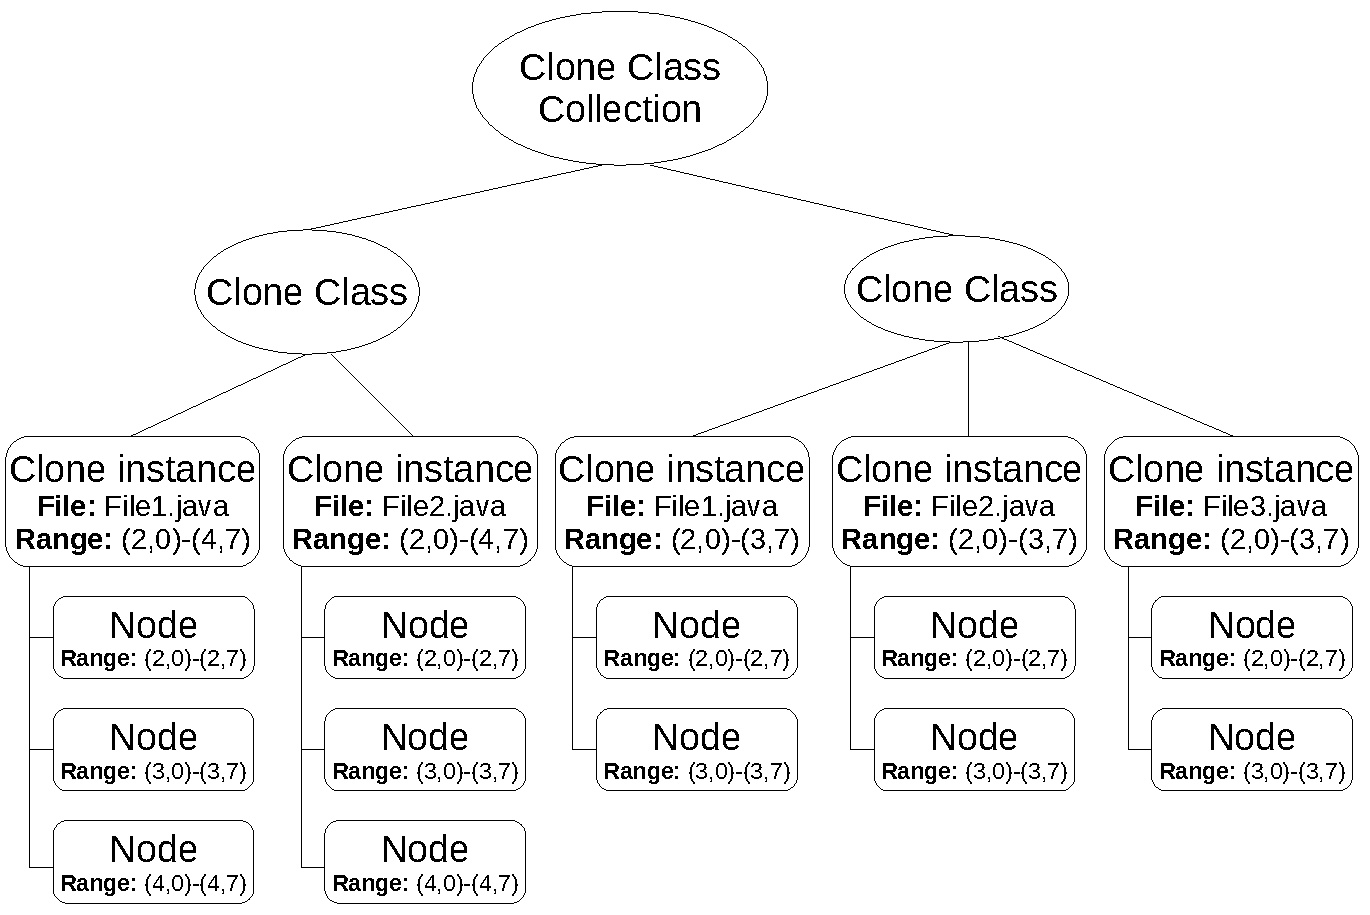
\includegraphics[width=1\columnwidth]{img/TerminologyExample}
  \caption{Representation of Figure~\ref{fig:cloneclasses} using the terminology introduced in Table~\ref{tab:clone-terminology}}
  \label{fig:terminologyexample}
\end{figure}

\subsection{Clone Classes vs Clone Pairs}\label{sec:classesvspairs}
In Table~\ref{tab:clone-terminology} we introduced the concept of clone classes. Clone classes consist of any number of clone instances. Some clone detection tools detect ``clone pairs'' instead, which consider each pair of clone instances separately. There are different reasons in literature whether clone pairs or clone classes should be considered for detection.

We decided to focus on \textit{clone classes} for our study, because of their advantages for refactoring. Clone pairs do not provide a general overview of all entities containing the clones, with all their related issues and characteristics~\cite{fontana2012duplicated}. Although clone classes are harder to manage, they provide all information needed to plan a suitable refactoring strategy, since this way all instances of a clone are considered. Another issue that results from grouping clones by pairs: the amount of clone references increases according to the binomial coefficient formula (two clones form a pair, three clones form three pairs, four clones form six pairs, and so on), which causes a heavy information redundancy~\cite{fontana2012duplicated}.

\section{Clone Types} \label{chap:backgroundclonetypes}
Duplication in code is found in many different forms. Most often duplicated code is the result of a programmer reusing previously written code \cite{haefliger2008code, baxter1998clone}. Sometimes this code is then adapted to fit the new context. To reason about these modifications, several clone types have been proposed. These clone types are described in Roy et al \cite{roy2007survey}:
\begin{displayquote}
\textbf{Type I:} Identical code fragments except for variations in whitespace (may be also variations in layout) and comments.\\
\textbf{Type II:} Structurally/syntactically identical fragments except for variations in identifiers, literals, types, layout and comments.\\
\textbf{Type III:} Copied fragments with further modifications. Statements can be changed, added or removed in addition to variations in identifiers, literals, types, layout and comments.
\end{displayquote}
A higher type of clone means that it's harder to detect and refactor. There are many studies that adopt these clone types, analyzing them further and writing detection techniques for them \cite{sajnani2016sourcerercc, kodhai2010detection, van2019novel}.

%\subsection{Type 4 clones}
%For this study we have chosen to take type 4 clones out of the scope, because they are both hard to detect and hard to refactor. % TODO: Sander - why is this the case?
%A study by Kodhai et al \cite{kodhai2013method} looks into the distribution of the different types of clones in several open source systems (see table 6 of his study). It becomes apparent that type 4 clones exist way less in source code than all of the other types of clones. For instance, for the J2sdk-swing system he finds 8115 type 1 clones, 8205 type 2 clones, 11209 type 3 clones and only 30 type 4 clones. Because of that, we can conclude that type 4 clones are relatively less relevant to study.
% TODO: Sander - Deze subsectie wil ik wel even over hebben, loopt niet helemaal lekker maar niet zo makkelijk uit te leggen

\section{Refactoring techniques}
In Martin Fowler's popular ``Refactoring'' book \cite{fowler2018refactoring}, he exclaims that \textit{``if you see the same code structure in more than one place, you can be sure that your program will be better if you find a way to unify them''}. He describes several techniques to deal with duplication, dependent on the context of the clone. In this section we describe the methods that we use in this study.

\subsection{Extract Method}
Current clone refactoring research shows that the ``Extract Method'' refactoring technique can refactor most duplication problems \cite{fontana2015duplicated, tsantalis2015assessing, white2016deep}. ``Extract Method'' moves matching functionality in method bodies to a common place, namely a new method \cite{fowler2018refactoring}. An example of this procedure is displayed in figure \ref{fig:extractmethod}.

\begin{figure}[H]
\begin{parcolumns}{2}
\colchunk[1]{
\begin{javacode}
// Original
public void doStuff(){
|\highlightYellow|  doA();
|\highlightYellow|  doB();
  doC();
|\highlightYellow|  doA();
|\highlightYellow|  doB();
}
\end{javacode}}
\colchunk[2]{
\begin{javacode}
// Refactored
public void doStuff(){
|\highlightYellow|  doAandB();
  doC();
|\highlightYellow|  doAandB();
}

public void doAandB(){
  doA();
  doB();
}
\end{javacode}}
\end{parcolumns}
\caption{Refactoring a clone class through method extraction.}
\label{fig:extractmethod}
\end{figure}

\subsection{Move method}
In the example of the previous section, both duplicated parts are in the same method. However, a study by Fontana et al. \cite{fontana2015duplicated} shows that this is most often not the case. Based on the relation between clone instances, the extracted method must be moved to be accessible by all locations of the clone instances. This can require different techniques.

\subsubsection{Pull up method}
A refactoring technique to move a method up in its inheritance structure is called ``Pull up method'' \cite{fowler2018refactoring}. This way, if cloned methods are related in any way through inheritance, they can be called by both classes by placing the method in a class they both have in common. This way its possible to refactor both fully cloned methods (by just pulling up the method) and partially cloned methods (by first performing method extraction and then pulling up the refactored method). Anexample of this refactoring method is shown in Figure~\ref{fig:pullupmethod}.

\begin{figure}[H]
\begin{parcolumns}{2}
\colchunk[1]{
\begin{javacode}
// Original
class Vehicle{
  void start(){
|\highlightYellow|    putKeyIn();
|\highlightYellow|    turnKey();
    drive();
  }
}

class Car extends Vehicle{
  void startEngine(){
|\highlightYellow|    putKeyIn();
|\highlightYellow|    turnKey();
  }
}
\end{javacode}}
\colchunk[2]{
\begin{javacode}
// Refactored
class Vehicle{
  void start(){
|\highlightYellow|    startEngine();
    drive();
  }

  void startEngine(){
|\highlightYellow|    putKeyIn();
|\highlightYellow|    turnKey();
  }
}

class Car extends Vehicle{
}
\end{javacode}}
\end{parcolumns}
\caption{Refactoring a clone class using ``Pull Up Method''.}
\label{fig:pullupmethod}
\end{figure}

\subsubsection{Create class abstraction based on implicit relations}
Duplication in source code is an implicit relation between fragments of source code. If two classes have many of these implicit relations, then the implementation should be refactored to make this relation explicit \cite{fowler2018refactoring}. If the classes do not yet have a parent/super class, a parent class can be created and the common functionality can be placed in this newly created class. This makes the relation between these classes explicit and reduces duplication.

\begin{figure}[H]
\begin{parcolumns}{2}
\colchunk[1]{
\begin{javacode}
// Original
class Truck{
  void startEngine(){
|\highlightYellow|    putKeyIn();
|\highlightYellow|    turnKey();
  }
}

class Car{
  void startEngine(){
|\highlightYellow|    putKeyIn();
|\highlightYellow|    turnKey();
  }
}
\end{javacode}}
\colchunk[2]{
\begin{javacode}
// Refactored
class Vehicle{
  void startEngine(){
|\highlightYellow|    putKeyIn();
|\highlightYellow|    turnKey();
  }
}

class Truck extends Vehicle{
}

class Car extends Vehicle{
}
\end{javacode}}
\end{parcolumns}
\caption{Refactoring a clone class using ``Create class abstraction''.}
\label{fig:createclassabstraction}
\end{figure}

\subsubsection{Providing default implementations for common functionality}
In Java, C\#, Python and possibly other object-oriented languages, the programmer can create interfaces of which a class can implement any number. Such interfaces can (in Java, C\# and Python) provide default implementations for common functionality \cite{mohnen2002interfaces}. This gives an opportunity to make the relation between classes explicit and reduce duplication. It can be used in instances where creating a new parent class for duplicated classes is undesirable. An example of this is shown in Figure~\ref{fig:createinterfaceabstraction}, in which two unrelated types (Human and Radio) share a common property (making sound).

\begin{figure}[H]
\begin{parcolumns}{2}
\colchunk[1]{
\begin{javacode}
// Original
class Human implements MakesSound{
  void broadcastNews(){
|\highlightYellow|    sayNews();
|\highlightYellow|    sayWeather();
  }
}

class Radio implements MakesSound{
  void broadcastNews(){
|\highlightYellow|    sayNews();
|\highlightYellow|    sayWeather();
  }
}

interface MakesSound{
  void sayNews();
  void sayWeather();
}
\end{javacode}}
\colchunk[2]{
\begin{javacode}
// Refactored
class Human implements MakesSound{
}

class Radio implements MakesSound{
}

interface MakesSound{
  default void broadcastNews(){
|\highlightYellow|    sayNews();
|\highlightYellow|    sayWeather();
  }

  void sayNews();
  void sayWeather();
}
\end{javacode}}
\end{parcolumns}
\caption{Refactoring a clone class creating a default implementation for common functionality.}
\label{fig:createinterfaceabstraction}
\end{figure}

%\subsection{Clone refactoring in relationship to its context}
%How to refactor clones is highly dependent on their context. Method-level clones can be extracted to a method \cite{kodhai2013method} if all occurrences of the clone reside in the same class. If a method level clone is duplicated among classes in the same inheritance structure, we might need to pull-up a method in the inheritance structure. If instances of a method level clone are not in the same inheritance structure, we might need to either make a static method or create an inheritance structure ourselves. So not only a single instance of a clone has a context, but also the relationship between individual instances in a clone class. This is highly relevant to the way in which the clone has to be refactored.

\section{Internal and external classes}
In this study we differentiate between \textit{internal} and \textit{external} classes. Classes are the components of a software system that contain its functionality. When analyzing a software system, \textit{Internal classes} are classes that belong to this software system specifically, and its source code is included in the project.

\textit{External classes} are classes that a software system uses but do not belong to this specific software system (but to an external dependency). Most often these external dependencies are referenced in a file that its build automation system uses to fetch a projects' dependencies.

Regarding refactoring, a software system can often not change the source code of its dependencies. This can sometimes be a burden, when an external dependency does not use proper abstractions that are required by a software system. In this study we take external classes into consideration when choosing a refactoring technique, to be sure not to modify them.

\subsection{Maven}
For this study we perform a shallow analysis on external dependencies, in order to derive more context for internally used concepts. As these external dependencies are most often not included in a software systems' source code, we must first use the projects' build automation system to gather the dependencies. To limit the scope of this process, we decided to focus on only the \textit{Maven}\footnote{Apache Maven is a build automation system mainly used for Java: \url{https://maven.apache.org/}} build automation system.

Maven is a build automation tool, mainly used with the Java programming language. Maven has a simple ecosystem to configure and fetch the binaries and source code of all software projects a given codebase is dependent on. Maven can also be used to run tests for the systems and to package the project as an executable file.

\section{(Object-Oriented) Programming Languages}
This section explains concepts, terminology and jargon of (object-oriented) programming languages that we use in this study.

\subsection{AST} \label{sec:astbackground}
An Abstract Syntax Tree (AST) is a tree consisting of an hierarchical representation of the source code of a program. Detecting code clones on the AST of a program allows for a deeper understanding of the concepts that are being analyzed. Having an AST, we know how concepts in the code are related. This helps to determine in what classes and methods cloned code is found.

Having access to a programs' AST also helps in the process of refactoring. Moving AST nodes rather than textual modifications reduces error margins because the tree structure stays intact.

The AST consists of nodes of the following types (examples are for Java):
\begin{itemize}
  \item \textbf{Declarations}: Method-declaration, class-declaration, etc.
  \item \textbf{Statements}: If-statement, switch-statement, expression-statement, etc.
  \item \textbf{Expressions}: Variables, literals, method calls, variable assignments, etc.
  \item \textbf{Types}: Primitives, reference types, void, etc.
  \item \textbf{Clauses}: Catch-clause, else-clause, etc.
\end{itemize}

\subsection{Inheritance}
Object-Oriented programming languages use inheritance to model real-world relations between data concepts. Inheritance allows an object to inherit all functionality from another object. For instance, a ``Car'' object would inherit functionality and data from generalized concepts, such as ``Vehicle''. Using inheritance it is possible to reduce duplication, as multiple objects can inherit common functionality.

When looking at the inheritance structure of a program, we can get a deeper understanding of a programs' architecture. The use of inheritance to group common functionality and data is called ``Abstraction''. Duplication in source code can be a result of an inadequate use of abstraction. Because of that, refactoring code clones might require to create such abstractions of common functionality.

\subsection{Code Quality}
Different programming languages have different ways to measure code quality. For object-oriented programming languages this largely comes in the form of code smells (patterns that should be avoided) and design patterns (patterns which may improve code design and comprehensibility when used correctly).

\subsubsection{Code Smells}
Code smells are patterns in code that should be avoided, because they have a negative effect on system design. Duplicate code is, among many others, one example of a code smell. Having many code smells present in source code can significantly increase maintainence costs of the source code or even render a software system unmaintainable. This increases technical debt: a debt present in the system the will have to be repaid at a later point of time. Such technical debt often comes at the expense of developing new features, fixing bugs and other aspects surrounding a programs functional behaviour.

\subsubsection{Design Patterns}
Most code smells have design patterns that can be used to mitigate the smell. For instance, duplicate code can be mitigated by using appropriate abstractions or refactoring duplicate code to a common place. Design patterns differ from refactoring methods in the sense that they are more about an architectural pattern rather than a certain kind of code modification.

\subsubsection{Maintainability Metrics}
Maintainability metrics are features of source code by which an indication of the maintainability of the source code can be measured. Heitlager at al. \cite{heitlager2007practical} propose a maintainability model that categorize the results of metrics into different ``score'' categories. For instance, with duplication, if 0-3\% of the project is duplicated, the project will get the highest score on a scale of 1 to 5 (only integers, no floating point numbers). Such a maintainability model is intuitive for measuring the quality of a software system, especially large software systems with a lot of source code to base the metrics on. However, this maintainability model \cite{heitlager2007practical} lacks in measuring fine-grained changes: most small changes will not fall into a different category. Because of that, this model is less suitable for measuring the impact of single refactorings.

\subsection{Java}
We run all our experiments on projects written in Java. Because of that, we get some information that is specific to Java systems. Additionally, we perform automated refactorings on Java systems, which requires the use of Java language concepts. These are explained in this section. Many of these concepts also exist in other programming languages, but often not in all.

\subsubsection{Interfaces}
Java uses the concept of interfaces to loosely couple a specification and its implementation. Interfaces are specifications about what a (group of) objects do. Often, methods don't need an entire object, but just use a few properties of it. Because of that, Java recommends to program to an interface rather than an implementation. This means that we should use abstractions of expected functionality rather than complete implementations of functionality. This can make switching implementations at a later point in time easier.

Often, duplication is the result of an inappropriate use of abstractions. Two methods might describe operations on types following the same contract, but because of a lack of abstraction the programmer may choose to clone such methods. This will result in duplicated methods with minor modifications to match a different implementation. Such duplicates can be mitigated by using proper abstractions, of which one option is to program methods against interfaces (contracts of expected functionality) rather than their full implementations.

\subsubsection{Packages}
Packages (sometimes called ``modules'' in other programming languages) are hierarchical groupings of related concepts. For instance, all UI logic in an application might go into the ``ui'' package. The ``ui'' package can have a subpackage named ``keyhandling'' for all keyhandling operations. These packages contain package-level declarations, like classes and interfaces. Names of class-level declarations must be unique within the package. However, duplicate declaration names may exists in subpackages and parent packages.

In Java, all declarations used from outside the package a declaration is in, must be \textit{imported}. Importing a declaration from outside the current package goes by the fully qualified identifier (FQI) of the declaration. The FQI of a declaration gives an unique identifier for a symbol in a codebase. For instance, if our ``keyhandling'' package would contain a ``KeyHandler'' class, its fully qualified identifier would be ``ui.keyhandling.KeyHandler''.

\subsubsection{Visibility}
In Java, we can protect declarations from being used in scopes in which they are supposed to be used. If a method should only be used within the class itself, we can give it a ``private'' visibility. If a method is to be used by its children in its inheritance hierarchy, we can set its visibility to ``protected''. If a method is supposed to be part of the public contract of an object, we can set it to ``public'' visibility. Alternatively, there is ``package'' visibility, for declarations that should only be referenced within the same package. This allows control over what parts of an application should be able to access what declarations.

\chapter{Related work} \label{ch:related_work}
In this chapter we present the work related to this study.

\section{Refactoring suggestion tooling}
We are novel in the introduction of a fully automated refactoring tool. However, several tools have already been proposed for refactoring suggestion. In this section we discuss these tools.

\subsection{SUPREMO}
A thesis by Golomingi~\cite{koni2001scenario} is the first to explore mapping the relation between clone instances to refactoring methods. In this thesis, the author analyses the refactoring methods described by Martin Fowler \cite{fowler1999refactoring}. Mapping these to relations between clones, this results in Table \ref{tab:relationrefactoring}.

\begin{table}[H]
\begin{tabular}{lllllllll}
                     & Ancestor   & \begin{tabular}[c]{@{}l@{}}Common\\ Hierarchy\end{tabular} & \begin{tabular}[c]{@{}l@{}}First\\ Cousin\end{tabular} & \begin{tabular}[c]{@{}l@{}}Same\\ Method\end{tabular} & Sibling    & \begin{tabular}[c]{@{}l@{}}Single\\ Class\end{tabular} & Superclass & Unrelated \\
Extract Method       & \checkmark & \checkmark                                                 & \checkmark                                             & \checkmark                                            & \checkmark & \checkmark                                             &            &           \\
Insert Method Call   &            &                                                            &                                                        & \checkmark                                            &            & \checkmark                                             &            &           \\
Insert Super Call    &            &                                                            &                                                        &                                                       &            &                                                        & \checkmark &           \\
Parameterization     & \checkmark & \checkmark                                                 & \checkmark                                             & \checkmark                                            & \checkmark & \checkmark                                             & \checkmark &           \\
Pull Up Method       & \checkmark & \checkmark                                                 & \checkmark                                             &                                                       & \checkmark &                                                        & \checkmark &           \\
Form Template Method & \checkmark & \checkmark                                                 & \checkmark                                             & \checkmark                                            & \checkmark & \checkmark                                             & \checkmark &           \\
Push Down Method     &            &                                                            &                                                        &                                                       &            &                                                        & \checkmark &           \\
Extract Superclass   &            & \checkmark                                                 & \checkmark                                             &                                                       & \checkmark &                                                        &            &
\end{tabular}
\caption{Mapping clone relations to refactoring techniques \cite{koni2001scenario}}
\label{tab:relationrefactoring}
\end{table}

The author then proposes a tool named ``SUPREMO''. This tool determines the relations between clone instances, computes the impact of the clones and proposes refactorings. Their tool features visualizations to show how clones are related in the inheritance structure. This tool is written for the Smalltalk programming language. The authors verify their approach by presenting several cases in which their tool analyses source code and outputs a refactoring suggestion.

\subsection{Duplicated Code Refactoring Advisor (DCRA)}
Fontana et al.~\cite{fontana2012duplicated, fontana2015duplicated} perform literature analyses to match clone context to refactoring opportunities. On basis of this literature study, they match refactoring methods \cite{fowler1999refactoring} to clone relations \cite{koni2001scenario}
The Duplicated Code Refactoring Advisor (DCRA) looks into refactoring opportunities for clone pairs~\cite{fontana2012duplicated, fontana2015duplicated}. DCRA only focuses on refactoring clone pairs, with the authors arguing that \textit{clone pairs are much easier to manage when considered singularly.} As intermediate steps, the authors measure a corpus of Java systems for some clone-related properties of the systems, like the relation (in terms of inheritance) between code fragments in a clone pair. We further look into these measurements in Sec.~\ref{chap:relationsinstances}.

A tool named Aries~\cite{higo2004aries, higo2008metric} focuses on the detection of refactorable clones. They do this based on the relation between clone instances through inheritance, similar to Fontana et al.~\cite{fontana2012duplicated}. This tool only proposes a refactoring opportunity and does not provide help in the process of applying the refactoring.

We investigated several research efforts that look into code clone refactoring~\cite{alwaqfi2017refactoring, chen2018clone, koni2001scenario}. However, all of these tools only support a subset of all harmful clones that are found. Also, these tools are limited to suggesting refactoring opportunities, rather than actually applying refactorings where suitable. Finally, all published approaches have limitations, such as false positives in their clone detection~\cite{chen2018clone} or being limited to clone pairs~\cite{higo2008metric}.

\chapter{Defining refactoring-oriented clone types}\label{chap:clonetypes}
In section \ref{chap:backgroundclonetypes} we introduced the four clone types as defined in literature. These simple definitions are suitable for analysis of a codebase. Their detection results in simple to understand numbers to argue about a codebase. However, these clone types have a few flaws which makes it hard to argue to what extend two fragements of code are functionally related. For each of type 1-3 clones~\cite{roy2007survey} we list our solutions to their shortcomings to increase the chance that we can refactor the clone while improving the design. Due to the serious challenges involved in their detection and refactoring, type 4 clones are not considered in this study.

We also look into clone detection tools for their suitability to support the proposed clone type definitions. We selected a few criteria  Most clone detection tools support these definitions of clone types. However, many of these tools use a vastly different approach. A study by Saini et al \cite{saini2018towards} outlines different clone detection tools and compares their results for each of type 1-3 clones. Even though they operate on the same type definitions, the tools used in this study yield different results.

\section{Shortcomings of clone types}
The clone definitions, as outlined in section \ref{chap:backgroundclonetypes}, allow reasoning about the duplication in a software system. Clones by these definitions can relatively easily and efficiently be detected. This has allowed for large scale analyses of duplication. However, these clone type definitions have shortcomings which makes the clones detected in correspondance with these definitions less valuable for (automated) refactoring purposes.

In this section we discuss the shortcomings of the different clone type definitions which make them less suitable for (automated) refactoring. Because of that, these clones require more judgement whether they should and can be refactored.

\subsection{Type 1 clones} \label{chap:type1clones}
Type 1 clones are \textit{identical clone fragments except for variations in whitespace and comments} \cite{roy2007survey}. This allows for the detection of clones that are the result of copying and pasting existing code, along with other reasons why duplicates might get into a codebase.

Type 1 clones are in most cases implemented as textual equality between code fragments (except for whitespace and comments). Although textually equal, method calls can still refer to different methods, type declarations can still refer to different types and variables can be of a different type. In such cases refactoring opportunities could be invalidated. An example of such a case is displayed in figure \ref{fig:type1}.

\begin{figure}[H]
  \includegraphics[width=1\columnwidth]{img/type1}
  \caption{Example of a type 1 clone.}
  \label{fig:type1}
\end{figure}

In the example in figure \ref{fig:type1}, we see a type 1 clone consisting of two methods. However, these clones might still be very hard to refactor as we cannot see by this example whether they are functionally equal. Both code fragments use different imported types, some of which imported via a wildcard. Because of this, it is hard to verify which of the used types have the same underlying implementation. This can make type 1 clones less suitable for refactoring purposes, as they require additional judgement regarding the refactorability of such a clone. When aiming to automatically refactor clones, applying refactorings to clones as shown in figure \ref{fig:type1}, is bound to be error prone and result in a uncompilable project or a difference in functionality.

Because of this, type 1 clones may not all be subject to refactoring. In section \label{chap:type1rclones} we describe an alternate approach towards detecting type 1 clones, which results in only clones that can be refactored.

\subsection{Type 2 clones}
Type 2 clones are \textit{structurally/syntactically identical fragments except for variations in identifiers, literals, types, layout and comments} \cite{roy2007survey}. This definition allows for the reasoning about code fragments that were copied and pasted, and then slightly modified. The two methods displayed in figure \ref{fig:type2} are type 2 clones of each other.

\begin{figure}[H]
  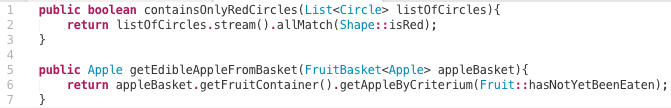
\includegraphics[width=1\columnwidth]{img/type2}
  \caption{Example of a type 2 clone.}
  \label{fig:type2}
\end{figure}

Looking at the example in listing \ref{fig:type2}, we see an example of a type 2 clone that poses no harm to the design of the system. Both methods are, except for their matching structure, completely different in functionality. They operate on different types, call different methods, return different things, etc. Having such a method flagged as a clone does not provide much useful information.

When looking at refactoring, type 2 clones can be very difficult to refactor. For instance if we have variability in types, the code can describe operations on two completely dissimilar types. Type 2 clones do not differentiate between primitives and objects, which makes the these clones often not so useful for refactoring purposes.

\subsection{Type 3 clones}
Type 3 clones are \textit{copied fragments with further modifications. Statements can be changed, added or removed in addition to variations in identifiers, literals, types, layout and comments} \cite{roy2007survey}. Detection of clones by this definition can be very hard, as it may be hard to detect whether a fragment was copied in the first place if it was severely changed. Because of this, most clone detection implementations of type 3 clones work on basis of a similarity threshold \cite{svajlenko2014evaluating, cordy2011nicad}. This similarity threshold has been implemented in different ways: textual similarity (for instance using levenshtein distance) \cite{lavoie2011automated}, token-level similarity of statement-level similarity.

Having a definition that allows for any change in code poses serious challenges on refactoring. A levenshtein distance of one can already change the meaning of a code fragment significantly, for instance if the name of a type differs by a character (and thus referring to different types).

\section{Refactoring-oriented clone types}
To resolve the shortcomings of clone types as outlined in the previous section, we propose alternative definitions for clone types to be directed at detecting clones that can and should be refactored. We have named these clones type 1R, 2R and 3R clones. These definitions share similarities with the literature definitions, the number of each type corresponds with the clone type it is modeled after. The ``R'' stands for refactoring-oriented (and may be less suitable for other analyses).

\subsection{Type 1R clones} \label{chap:type1rclones}
We propose an alternative definition of type 1 clones. This definition requires cloned fragments to be not just textually equal, but also functionally equal. Although requiring fragements to be functionally equal, type 1R clones do not allow for change in implementation (like type 4 clones). We check functional equality of two fragments by validating the equality of the fully qualityfied identifier for referenced types, methods and variables. Type 1R clones are always a subset of type 1 clones.

\subsubsection{Referenced Types}
Many object-oriented programming languages (like Java, Python, C\#) require the programmer to import a type (or the class in which it is declared) before it can be used. Based on what is imported, the meaning of the name of a type can differ. For instance, if we import \texttt{java.util.List}, we get the interface which is implemented by all list datastructures in Java. However, importing \texttt{java.awt.List}, we get a listbox GUI component for the Java Abstract Window Toolkit (AWT). Because of this, for type 1R clones, we compare the fully qualified identifier for all referenced types.

\subsubsection{Called methods}
A codebase can have several methods with the same name. The implementation of these methods might differ. When we call two methods with an identical name, we can in fact call different methods. This is another reason that textually identical code fragements can differ functionally.

Because of this, for type 1R clones, we compare the fully qualified method signature for all method references. A fully qualified method signature consists of the fully qualified name of the method, the fully qualified type of the method plus the fully qualified type of each of its arguments. For instance, an \texttt{eat} method could become \texttt{java.lang.Boolean com.simonbaars.fruitgame.Apple.eat(java.util.List<com.simonbaars.fruitgame.tools.Tool>)}.

\subsubsection{Variables}
In typed programming languages, each variable declaration should declare a name and a type. When we reference a variable, we only use its name. If, in different code fragments, we use variables with the same name but different types, the code can be functionally unequal but still textually equal. As an example, see the code in figure \ref{lst:type1variables}.

\begin{figure}[H]
  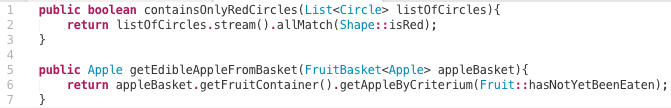
\includegraphics[width=1\columnwidth]{img/type2}
  \caption{Variables with different types but the same name.}
  \label{fig:type1variables}
\end{figure}

The body of both methods in figure \ref{lst:type2variables} is equal. However, their functionality is not. The first method adds two numbers together and the other concatenates an integer to a String.

For type 1R clones variable references should be compared by both type and name.

\section{Type 2R clones}
Type 2R clones are modelled after type 2 clones, which allow any change in identifiers, literals, types, layout, and comments. For refactoring purposes, this definition is unsuitable; if we allow any change in identifiers, literals, and types, we cannot distinguish between different variables, different types and different method calls anymore. This could render two methods that have an entirely different functionality as clones (as shown in figure \ref{fig:type2} previously). Refactoring such clones can be harmful instead of helpful.

We tackle these problems with type 2R clones to be able to detect such clones that can and should be refactored. Type 1R clones are a subset of type 2R clones. All rules that apply to type 1R clones also apply to type 2R clones. Additionally, type 2R clones allow variability in literals, variables and method calls. This variability however is constrained by a threshold. Type 2R do not allow any variability in types, as opposed to type 2 clones which do allow variability in types.

\subsubsection{A threshold for variability in literals, variables and method calls}
Type 2 clones allow any variability in literals, variables and method identifiers. However, this information tells a lot about the meaning of the code fragment. Most clone detection tools do not differentiate between a type 2 clone that differs by a single literal/identifier and one that differs by many. However, this does have a big impact on the meaning of the code fragment and thus the harmfulness of the duplication being there.

For type 2R clones we define a threshold for variability in literals, variables and method calls. We calculate the variability in literals, variables and method calls using the following formula:

T2R Variability = (Diff(l) + Diff(v) + Diff(m))/Total(t)
Diff = Amount that differ from other clone instances in the clone class
Total = Total number in the clone instance
l = Number of literals
v = Number of variables
m = Number of method calls
t = Number of tokens

Looking at this formula, it becomes apparent that we made the decision to let literals, variables and method calls count towards the same threshold. So a large variability in method calls might constrain variability from literals. This is because how to refactor variability in literals, variables and method calls. When we use either a different literal, variable or method call, we will have to use a 

\paragraph{Literal variability}


\subsubsection{Allow any change in some identifiers}
- Identifier of method declarations
- Identifier of locally declared variables
- Identifier of class/interface/enum declaration
- etc?

\begin{itemize}
  \item \textbf{Considering types:} Type 2 clones do not consider types. However, this can make a code fragment very hard to refactor, as different types can describe different functional concepts. Because of this, we propose that type 2R clones should consider types like type 1R clones do.
  \item \textbf{Having a distinction between different variables:} For type 2 clones, no identifiers would be taken into account. We agree that a difference in identifiers may still result in a harmful clone, but we should still consider the distinction between different variables. For instance, if we call a method like this: \texttt{myMethod(var1, var2)}, or call this method like this: \texttt{myMethod(var1, var1)}. Even if the variables have the same type, the distinction between the variables is important to ensure the functionality is the same after refactoring.
  \item \textbf{Defining a threshold for variability in literals:} For type 2 clones no literals would be taken into account. We agree, as when refactoring the clone (for example by extracting a method), we can turn the literal into a method parameter. However, we would argue that thresholds matter here. How many literals may differ for the segment still to be considered a clone with another segment? We need to define a threshold to be sure that, by refactoring, we are not replacing a code fragment by a worse maintainable design.
  \item \textbf{Consider method call signatures and define a threshold for variability in method calls:} As type-2 clones allow changes in identifiers, also the names of called methods may vary. However, because of this, completely different methods can be called in cloned fragments as a result. This poses serious challenges on refactoring and makes it more disputable whether such a clone is harmful for the maintainability of the code. This is because different method identifiers can describe a completely different functionality. Therefore, we suggest considering the call signatures of cloned methods when they are compared. We can allow variability in the rest of method identifiers by passing the function as a parameter. To limit the amount of parameters required we also recommend defining a threshold for variability in method call expressions, so only a limited number of method calls can vary.
\end{itemize}

\section{Type 3R clones}
Type 3 clones are even more permissive than type 2 clones, allowing added and removed statements. For these clones, thresholds matter a lot to make sure that not the whole project is detected as a clone of itself. The main question for this study regarding type 3 clones is: \textit{``how can we refactor type 3 clones while improving the design?''}.

Clone instances in type 3 clones are almost always different in functionality. As we have to ensure equal functionality after refactoring the clone, we have to wrap the difference in statements between the clone instances in conditional blocks. We can then pass a variable to indicate which path should be taken through the code (either a boolean or an enumeration). Such a refactoring would make added statements that are contiguous less harmful for the design than added statements that are scattered throughout the cloned fragment.

We also argue that statements that are not common between two clone instances, should not count towards the size of the clone (and thus towards the threshold which determines whether the clone will be taken into account). As for the detection of type 3 clones, we think the easiest opportunity to detect these clones is to consider it as a postprocessing step after clone detection. By trying to find short gaps between clones, we can find opportunities to refactor clone classes into a single type 3 clone class. The amount of statements that this ``short gap'' can maximally span should be dependent on a threshold value.

\section{The challenge of detecting these clones}\label{chap:challenge}
To detect each type of clone, we need to parse the fully qualified identifier of all types, method calls and variables. This comes with serious challenges, regarding both performance and implementation. Also, to be able to parse all fully qualified identifiers, and trace the declarations of variables, we might need to follow cross file references. The referenced types/variables/methods might even not be part of the project, but rather of an external library or the standard libraries of the programming language. All these factors need to be considered for the referenced entity to be found, on basis of which a fully qualified identifier can be created.

\section{Unifying the types}
In this chapter we have proposed refactoring-oriented definitions using the type 1, 2 and 3 clone definitions from literature as a baseline. In literature, these definitions are mainly aimed towards reasoning about duplication in source code. When considering these types for refactoring, the goal becomes slighly different. Because of this, having separate clone type definitions does not have any value. Rather, we need a single clone type definition by which we can detect all clones that can and should be considered for refactoring.

Because of this, the ultimate goal would be not to consider type 1R, 2R and 3R separately, but together. However, this is dependent on good thresholds for the type 2R variability and type 3R gap size. Because of this, we have dedicated section \ref{sec:thresholds} to performing measurements to find good thresholds. The ultimate goal is to have a single unified definition of clones that can and should be refactored. Although it will be next to impossible to define such a definition and its corresponding thresholds that does not detect false positives. However, we strive to find at least a near-optimal set of thresholds regarding the type definitions proposed in this chapter.

\section{Suitability of existing Clone Detection Tools towards our refactoring purposes}
\label{ch:tool-overview}
We conducted a short survey on (recent) clone detection tools that we could use to analyze refactoring possibilities. The results of our survey are displayed in table~\ref{table:dettools}. We chose a set of tools that are open source and can analyze a popular object-oriented programming language. Next, we formulate the following four criteria by which we analyze these tools:
\begin{enumerate}
    \item \textbf{Should find clones in any context.} Some tools only find clones in specific contexts, such as only method-level clones. We want to perform an analysis on all clones in projects to get a complete overview.
\item \textbf{Should find all clones in created control projects.} We assembled a number of test projects to assess the validity of clone detection tools. On basis of this, we checked whether clone detection tools can correctly find clones in diverse contexts.
\item \textbf{Can analyse resolved symbols.} When detecting clones for refactoring purposes, it is important that clone instances can be refactored. Sometimes, textual equality between code fragments does not imply that these can be refactored (this is described more elaborately in section \ref{chap:type1clones}). Because of this, we want to use a clone detection tool that can analyze such structures.
\item \textbf{Extensive detection configuration.} We aim to exclude expressions/statements from matching (more about our rationale in section~\ref{chap:clonetypes}). To achieve this, the tool needs to be able to allow those threshold changes. This can be either through simple changes of the source code, or by using some configuration file.
\end{enumerate}

\begin{table}[H]
 \begin{center}
  \caption{Our survey on clone detection tools.} \label{table:dettools}
  \medskip
\begin{tabular}{|l|l|l|l|l|l|}
\hline
\textbf{Clone Detection Tool} & \textbf{(1)} & \textbf{(2)} & \textbf{(3)} & \textbf{(4)} \\ \hline
Siamese \cite{ragkhitwetsagul2019siamese} &  &             &             & \checkmark            \\ \hline
NiCAD \cite{roy2008nicad, cordy2011nicad} & \checkmark                             & \checkmark            &             &             \\ \hline
CPD \cite{roy2009comparison} & \checkmark & \checkmark            &             &             \\ \hline
\begin{tabular}[c]{@{}l@{}}CCFinder \cite{kamiya2002ccfinder}\\ D-CCFinder \cite{livieri2007very}\end{tabular} & \checkmark  & \checkmark   &    &   \\ \hline
CCFinderSW \cite{semura2017ccfindersw}   & \checkmark     &             &             & \checkmark            \\ \hline
\begin{tabular}[c]{@{}l@{}}SourcererCC \cite{sajnani2016sourcerercc}\\ Oreo \cite{saini2018oreo}\end{tabular} & \checkmark    &             &             & \checkmark            \\ \hline
BigCloneEval \cite{svajlenko2016bigcloneeval}  & \checkmark  & \checkmark   &             &             \\ \hline
Deckard \cite{jiang2007deckard} & \checkmark   &             & \checkmark            &             \\ \hline
Scorpio \cite{higo2013revisiting, kamalpriya2017enhancing} & \checkmark   &     & \checkmark  & \checkmark   \\ \hline
\end{tabular}
\end{center}
\end{table}

None of the state-of-the-art tools we identified implement all our criteria, so we decided to implement our own clone detection tool: CloneRefactor\footnote{CloneRefactor (WIP) is available on GitHub: \url{https://github.com/SimonBaars/CloneRefactor}. This repository contains all scripts that were used to retrieve the data that is displayed in this paper.}.

\chapter{Evaluation setup}
In this chapter we describe the setup we use for our experiments. Our most prominent contribution is the proposal of a tool called CloneRefactor. This tool allows us to map clones with all clone definitions as described in chapter \ref{chap:clonetypes}.

All data for our experiments, as displayed in chapter \ref{ch:results}, is measured over a corpus of Java projects. In this chapter we will explain how we prepared this corpus.

\section{CloneRefactor}
CloneRefactor is the name of our clone detection and refactoring tool. It features the following novel functions:
\begin{itemize}
  \item Detection of clone classes rather than clone pairs.
  \item A novel detection method, aimed at extensibility.
  \item Detection of refactoring-oriented clone types, in addition to the literature clone types.
  \item Allows for automated refactoring of a subset of the detected duplication issues.
\end{itemize}
In this section we describe our approach and rationale for the design decisions regarding this tool.

\subsection{JavaParser}
A very important design decision for CloneRefactor is the usage of a library named JavaParser \cite{tomassetti2017javaparser}. JavaParser is a Java library which allows to parse Java source files to an abstract syntax tree (AST). JavaParser allows to modify this AST and write the result back to Java source code. This allows us to apply refactorings to the detected problems in the source code.

Integrated in JavaParser is a library named SymbolSolver. This library allows for the resolution of symbols using JavaParser. For instance, we can use it to trace references (methods, variables, types, etc) to their declarations (these referenced identifiers are also called ``symbols''). This is very useful for the detection of our refactoring-oriented clone types, as they make use of the fully qualified identifiers of symbols.

In order to be able to trace referenced identifiers SymbolSolver requires access to not only the analyzed Java projects, but also all its dependencies. This requires us to include all dependencies with the project. Along with this, SymbolSolver solves symbols in the JRE System Library (the standard libraries coming with every installation of Java) using the active Java Virtual Machine (JVM). This has a big impact on performance efficiency.

Because of the requirement of symbol resolution, the refactoring-oriented clone types are less suitable for large scale clone analysis.

\subsection{Clone Detection}
To detect clones, CloneRefactor parses the AST aqcuired from JavaParser to an unweighted graph structure. On basis of this graph structure, clones are detection. Dependent on the type of clones being detected, transformations may be applied. The way in which CloneRefactor was designed does not allow for several clone types to be detected simultaneously, in accordance with our clone type philosophy as described in chapter \ref{section:clonephilosophy}.

\subsection{Type specific transformations}

\section{The corpus}\label{chap:corpus}
For our measurements we use a large corpus of open source projects \cite{githubCorpus2013}. This corpus has been assembled to contain relatively higher quality projects. Also, any duplicate projects were removed from this corpus. This results in a variety of Java projects that reflect the quality of average open source Java systems and are useful to perform measurements on.

As indicated in chapter \ref{chap:challenge} CloneRefactor requires all libraries of software projects we test. As these are not included in the used corpus \cite{githubCorpus2013}, we decided to filter the corpus to only include Maven projects. Maven is a build automation tool used primarily for Java, and works on basis of an \texttt{pom.xml} file to describe the projects' dependencies. As no \texttt{pom.xml} files are included in the corpus, we cloned the latest version of each project in the corpus. We then removed each project that has no \texttt{pom.xml} file. As a final step, we collected all dependencies for each project by using the \texttt{mvn dependency:copy-dependencies -DoutputDirectory=lib} Maven command, and removed each project for which not all dependencies were available (due to non-Maven dependencies being used or unsatisfiable dependencies being referenced in the \texttt{pom.xml} file).

Some general data regarding this corpus is displayed in Table \ref{table:general}.

\begin{table}[H]
  \begin{center}
  \caption{General results for GitHub Java projects corpus \cite{githubCorpus2013}.} \label{table:general}
  \medskip
\begin{tabular}{|l|l|}
\hline
Amount of projects                                                                                      & 1,361      \\ \hline
\begin{tabular}[c]{@{}l@{}}Amount of lines (excluding\\whitespace, comments and newlines.)\end{tabular} & 1,414,996  \\ \hline
Amount of statements/declarations                                                                       & 1,212,189  \\ \hline
\begin{tabular}[c]{@{}l@{}}Amount of tokens (excluding\\whitespace, comments and newlines.)\end{tabular} & 11,643,194 \\ \hline
\end{tabular}
\end{center}
\end{table}

\chapter{CloneRefactor} \label{ch:clonerefactor}
% We bridged a gap between clone detection and refactoring .. by designing a tool
CloneRefactor is the name of our clone detection and refactoring tool. It features the following novel functions:
\begin{itemize}
  \item Detection of clone classes rather than clone pairs.
  \item A novel detection method, aimed at extensibility.
  \item Detection of refactoring-oriented clone types, in addition to the literature clone types.
  \item Allows for automated refactoring of a subset of the detected duplication issues.
\end{itemize}
In this section we describe our approach and rationale for the design decisions regarding this tool.

\begin{figure}[H]
  \centering
  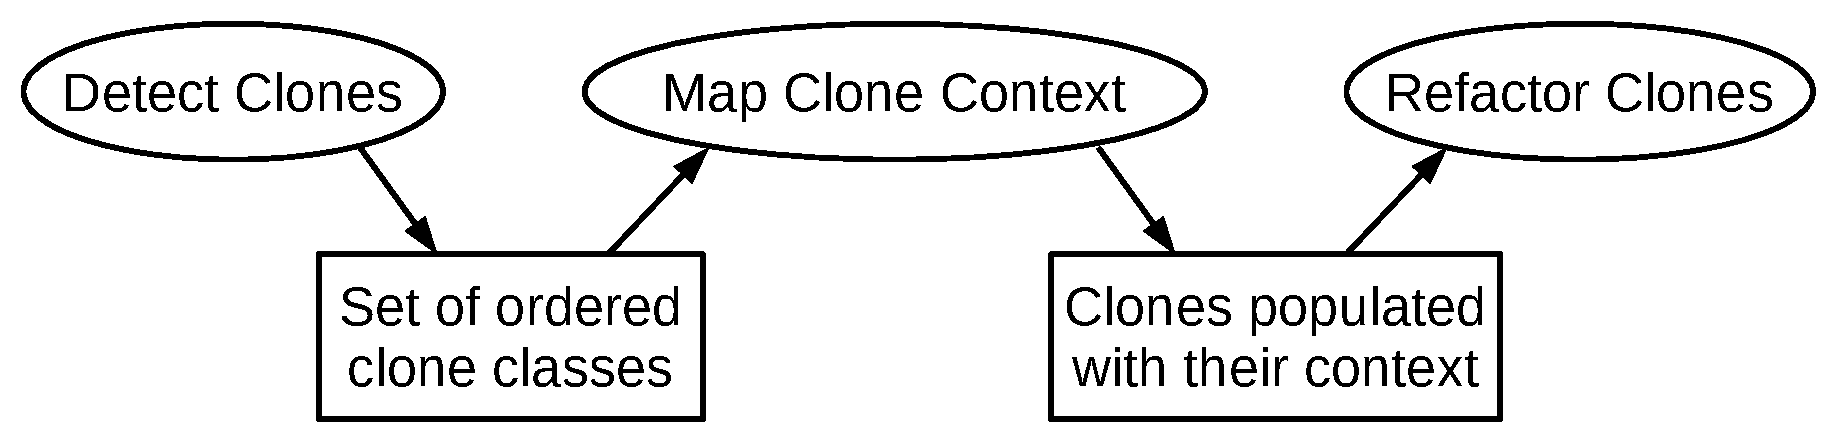
\includegraphics[width=0.8\columnwidth]{img/CloneRefactorOverall}
  \caption{CloneRefactor overall process.}
  \label{fig:clonerefactorprocess}
\end{figure}

Figure \ref{fig:clonerefactorprocess} shows the overall process used by CloneRefactor. First, we detect clones on basis of a Java codebase, given a Java project from disk and a configuration. The clone detection process is further explained in section \ref{sec:clonedetection}. After all clones are found, CloneRefactor maps the context of the clones. On basis of this context, CloneRefactor applies transformations to the source code for clones for which we have configured a refactoring.

\section{JavaParser}
A very important design decision for CloneRefactor is the usage of a library named JavaParser \cite{tomassetti2017javaparser}. JavaParser is a Java library which allows to parse Java source files to an abstract syntax tree (AST\footnote{An AST is a tree-representation of a source code file.}). JavaParser allows to modify this AST and write the result back to Java source code. This allows us to apply refactorings to the detected problems in the source code.

Integrated in JavaParser is a library named SymbolSolver. This library allows for the resolution of symbols using JavaParser. For instance, we can use it to trace references (methods, variables, types, etc) to their declarations (these referenced identifiers are also called ``symbols''). This is very useful for the detection of our refactoring-oriented clone types, as they make use of the fully qualified identifiers of symbols.

In order to be able to trace referenced identifiers SymbolSolver requires access to not only the analyzed Java projects, but also all its dependencies. This requires us to include all dependencies with the project. Along with this, SymbolSolver solves symbols in the JRE System Library (the standard libraries coming with every installation of Java) using the active Java Virtual Machine (JVM). This has a big impact on performance efficiency.

Because of the requirement of symbol resolution, the refactoring-oriented clone types are less suitable for large scale clone analysis.

\section{Thresholds}\label{sec:clonerefactorthresholds}
CloneRefactor operates on a set of thresholds to determine the validity of clones that are found. In general, these thresholds are:
\begin{itemize}
  \item \textbf{Minimum Amount of Nodes}: The minimum amount of nodes that should be in each instance of cloned fragements for them to be considered a clone class.
  \item \textbf{Minimum Amount of Tokens}: The minimum amount of tokens that should be in each instance of cloned fragements for them to be considered a clone class.
  \item \textbf{Minimum Amount of Lines}: The minimum amount of lines that should be in each instance of cloned fragements for them to be considered a clone class.
\end{itemize}

When we analyze type 2R or type 3R clones we use the following additional threshold:
\begin{itemize}
  \item \textbf{T2R Variability}: The percentage of variability we allow in variables, method calls and literals. How this threshold is calculated is explained in section \ref{sec:t2rcheckglobalthres}.
\end{itemize}

When we analyze type 3 or type 3R clones we use the following additional threshold:
\begin{itemize}
  \item \textbf{T3R Gap Size}: The size of the gap we allow between two valid clones. This is a percentage of the size of the gap against the size of both clones combined. How this threshold is calculated is further explained in section \ref{sec:t3rclonerefactor}.
\end{itemize}

\section{Clone Detection}\label{sec:clonedetection}
To detect clones, CloneRefactor parses the AST aqcuired from JavaParser to an unweighted graph structure. On basis of this graph structure, clones are detection. Dependent on the type of clones being detected, transformations may be applied. The way in which CloneRefactor was designed does not allow for several clone types to be detected simultaneously, in accordance with our clone type philosophy as described in chapter \ref{sec:unifying}.

The overall process regarding clone detection is displayed in figure \ref{fig:clonedetection}. First of all, we use JavaParser to read a project from disk and build an AST, one class file at a time. Each AST is then converted to a directed graph that maps relations between statements, further explained in section \ref{sec:clonegraph}. On basis of this graph, we detect clone classes and verify them using three thresholds (in order of importance):
\begin{itemize}
  \item Amount of tokens.
  \item Amount of statements.
  \item Amount of lines.
\end{itemize}
If the detection was configured to detect either type 2R, 3 or 3R clones we perform some type specific transformations on the resulting set of clones.

\begin{figure}[H]
  \centering
  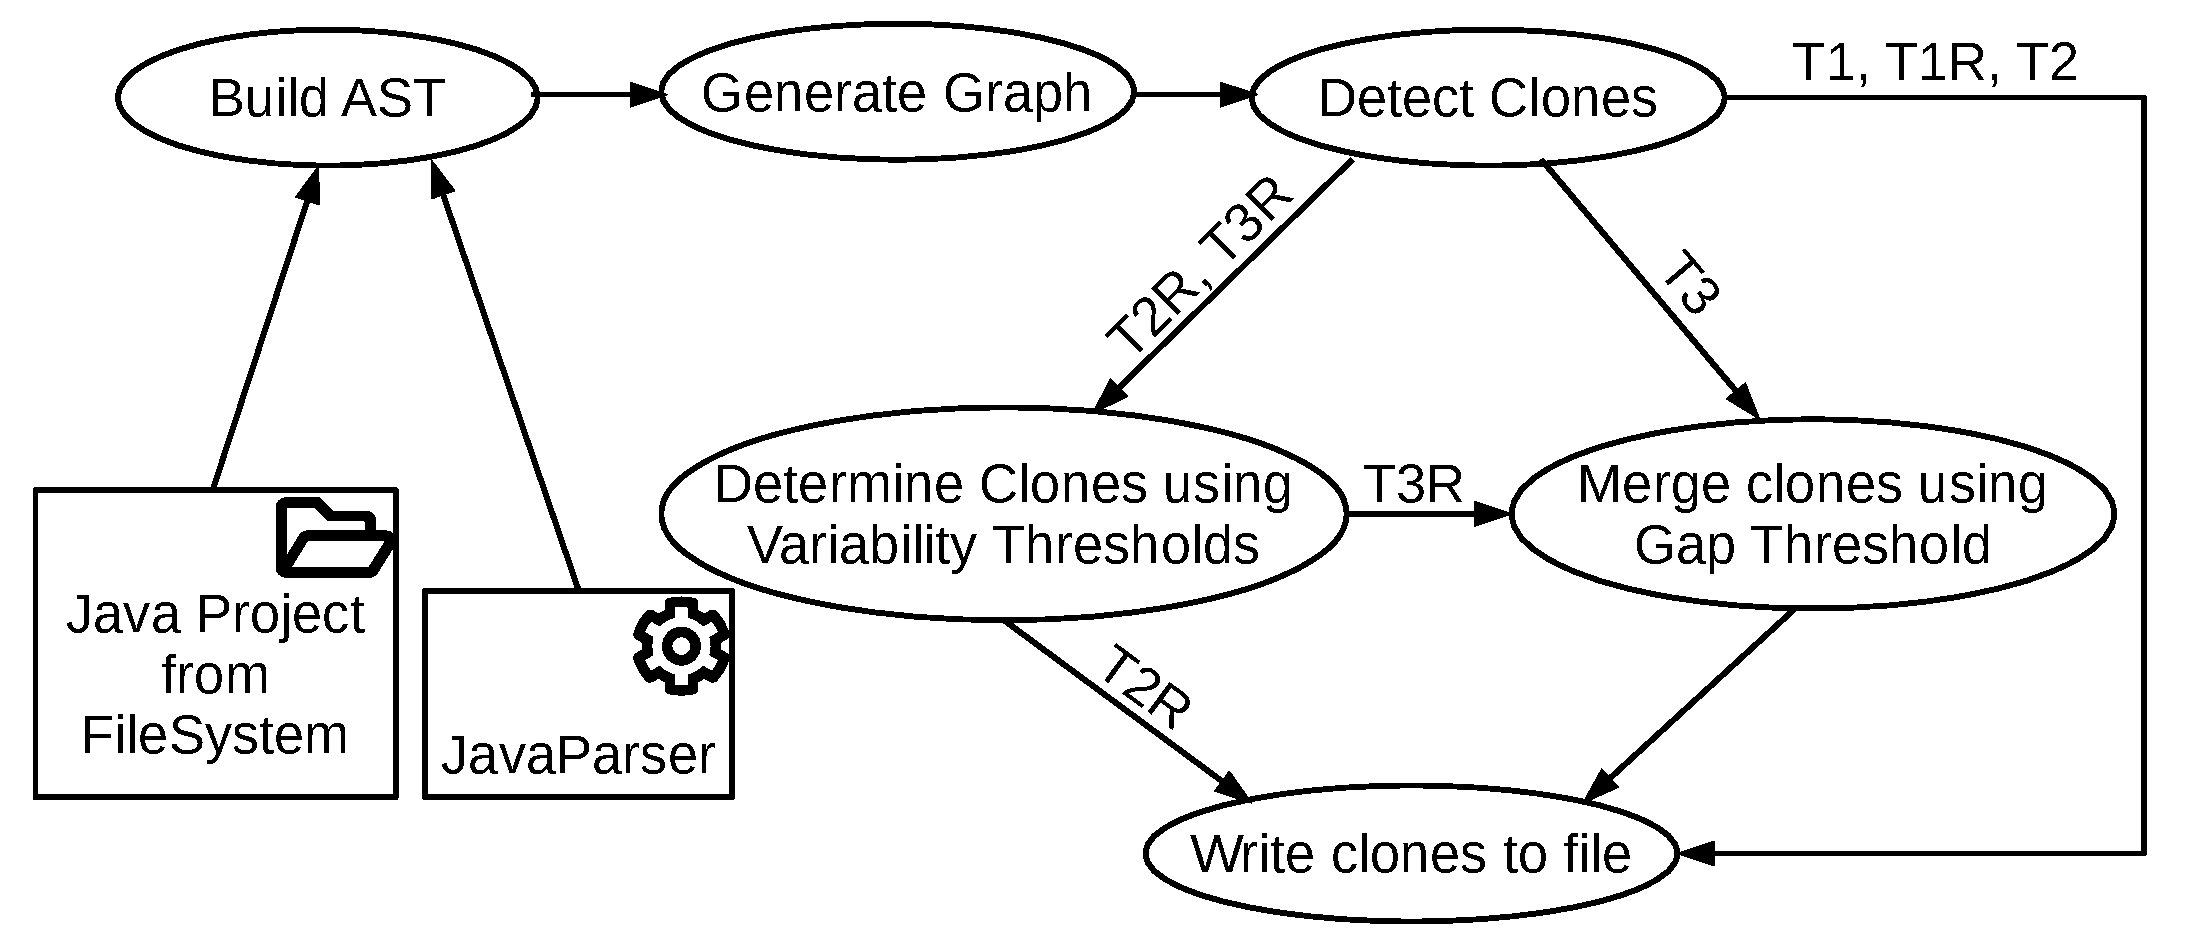
\includegraphics[width=1\columnwidth]{img/CloneDetection}
  \caption{CloneRefactor clone detection process.}
  \label{fig:clonedetection}
\end{figure}

\subsection{Generating the clone graph}\label{sec:clonegraph}
First of all, we parse the AST obtained from JavaParser into a directed graph structure. We have chosen to base our clone detection around statements as the smallest unit of comparison. This means that a single statement cloned with another single statement is the smallest clone we can find. The rationale for this lies in both simplicity and performance efficiency. This means we won't be able to find when a single expression matches another expression, or even a single token matching another token. This is in most cases not a problem, as expressions are often small and do not span the minimal size to be considered a clone in the first place (more about this in section \ref{sec:thresholds}).

\subsubsection{Filtering the AST}
As a first step towards building the clone graph, we preprocess the AST to decide which AST nodes should become part of the clone graph. We have decided to consider declarations and statements as the smallest compared entities. The main reasoning for this is because considering smaller AST constructs, like expressions, significantly increases the complexity and CPU usage of our clone detection and refactoring efforts.

Additionally, we exclude package declarations and import statements. These are omitted by most clone detection tools, as clones in import statements hold limited valuable information.

\subsubsection{Building the clone graph}\label{sec:buildingclonegraph}
Building the clone graph consists of walking the AST in-order for each declaration and statement. For each declaration/statement found, we map the following relations:
\begin{itemize}
  \item The declaration/statement preceding it.
  \item The declaration/statement following.
  \item The last \textbf{preceding} declaration/statement with which it is cloned.
\end{itemize}
We do not create a separate graph for each class file, so the statement/declaration preceding or following could be in a different file. While mapping these relations, we maintain a hashed map containing the last occurrence of each unique statement. This map is used to efficiently find out whether a statement is cloned with another. An example of such a graph is displayed in figure \ref{fig:clonegraphsimple}.

\begin{figure}[H]
  \centering
  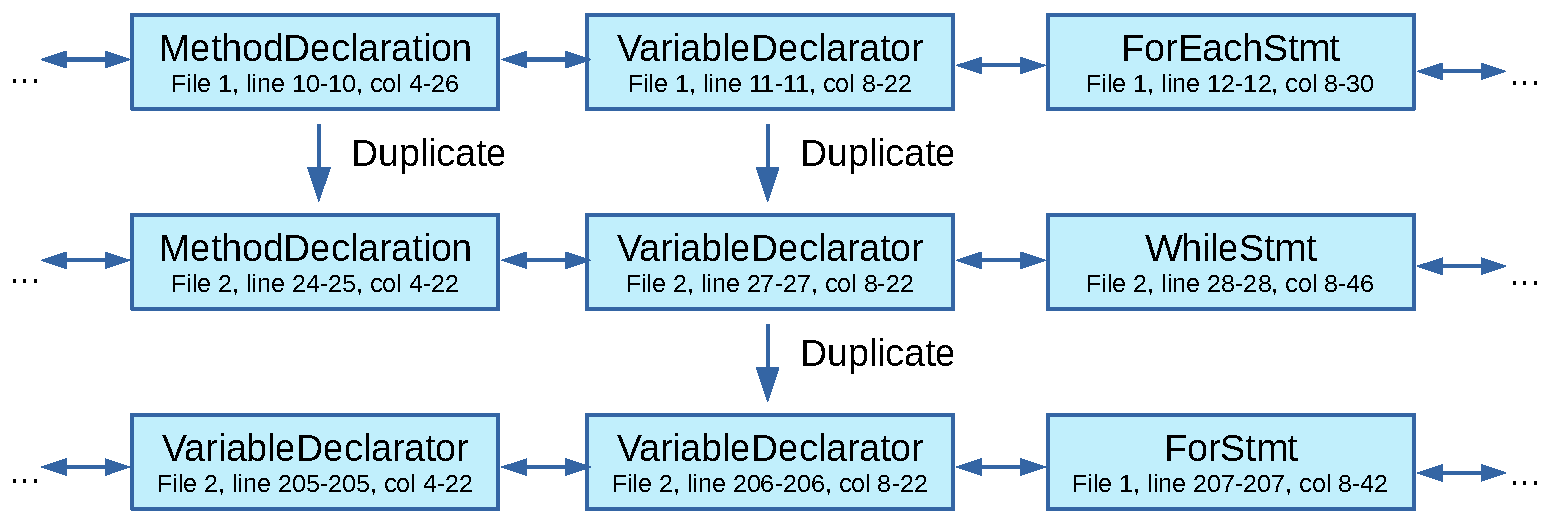
\includegraphics[width=1\columnwidth]{img/CodeGraph2}
  \caption{Abstract example of a part of a possible clone graph as built by CloneRefactor.}
  \label{fig:clonegraphsimple}
\end{figure}

We refer to the declarations and statements in this graph as \textit{nodes}. The relations \textit{next} and \textit{previous} in this graph are represented as an twodirectional arrow. The relations representing duplication are directed. This is a restriction we've chosen as it creates an important constraint for the clone detection process. This process is explained in section \ref{sec:detectingclones}.

\subsubsection{Comparing Statements/Declarations} \label{sec:comparingstuff}
In the previous section we described a ``duplicate'' relation between nodes in the clone graph built by CloneRefactor. Whether two nodes in this graph are duplicates of each other is dependent on the clone type. In this section, we will describe for each type how we compare statements and declarations to assess whether they are clones of each other.

CloneRefactor detects six different types of clones: T1, T2, T3, T1R, T2R and T3R. These types are further explained in chapter \ref{chap:clonetypes}. For \textbf{type 1} clones, CloneRefactor filters the tokens of a node to exclude its comments, whitespace and end of line (EOL) characters and then compares these tokens. For \textbf{type 2} clones, the tokens are further filtered to omit all identifiers and literals. \textbf{Type 3} clones do the same duplication comparison as type 2 clones.

For \textbf{type 1R} clones, this comparison is a lot more advanced. For \textit{method calls} we trace their declaration and use its fully qualified method signature for comparison with other nodes. For all \textit{referenced types} we trace their declarations and use assemble their fully qualified identifier for comparison with other nodes. For \textit{variables} we trace their declaration and their types. If the variable type is a primitive we can directly use it for comparison. If it is a referenced type, we have to trace this type first in order to collect their fully qualified identifier for comparison.

\textbf{Type 2R} clones allow any variation in literals, variables and method calls at this stage in the clone detection process. However, for \textit{literals} we do resolve their type in order to verify that they are of the same type. For \textit{variables} we also only verify that their types are the same (but not their names). For \textit{method calls}, we trace their declaration but only compare the fully qualified identifier for its return type and each of its arguments' types. Apart from that, we do not compare the names of method, class, interface and enum declarations.

In this stage, \textbf{type 3R} clones have the same compare rules as type 2R clones.

\subsubsection{Mapping graph nodes to code}
The clone graph, as explained in section \ref{sec:buildingclonegraph}, contains all declarations and statements in a source code. However, declarations and statements may themselves have child declarations and statements. To avoid redundant duplication checks, we exclude child declarations and statements from each node. Look at figure \ref{fig:clonegraph} for an example of how source code maps to AST nodes.

\begin{figure}[H]
  \centering
  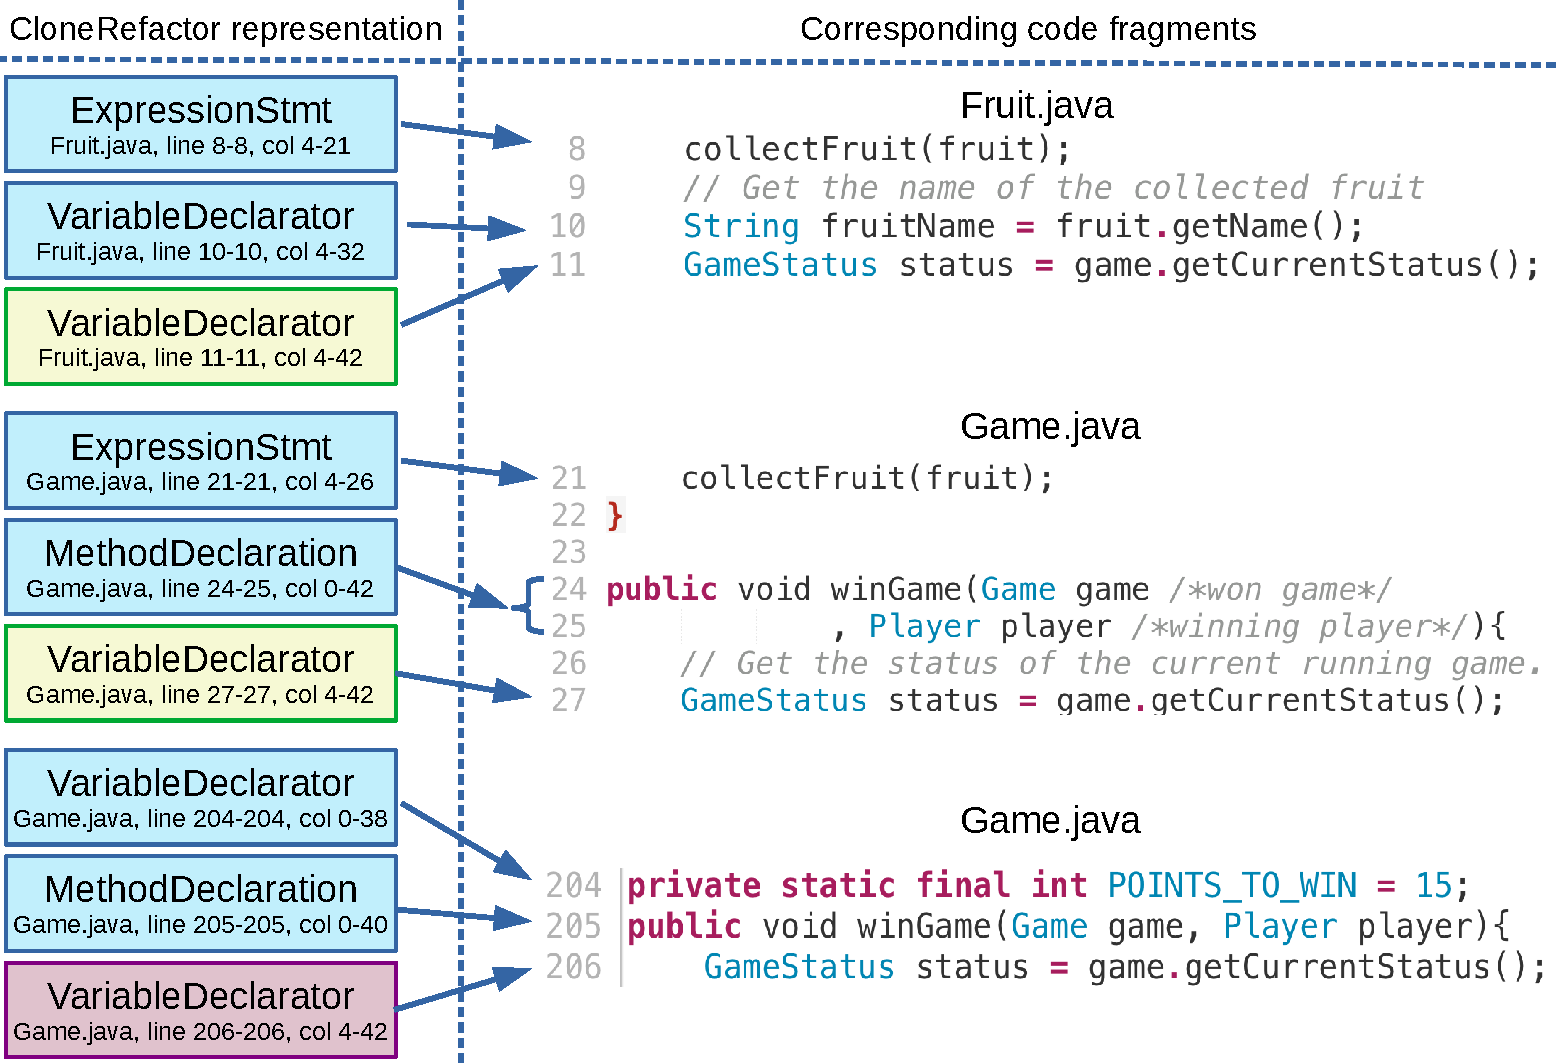
\includegraphics[width=1\columnwidth]{img/CloneGraphCode}
  \caption{CloneRefactor extracts statements and declarations from source code.}
  \label{fig:clonegraph}
\end{figure}

In line 24-25 of the code fragment, we see a \texttt{MethodDeclaration}. The node corresponding with this MethodDeclaration denotes all tokens found on these two lines, line 24 and 25. Although the statements following this method declaration (those that are part of its body) officially belong to the method declaration, they are not included in its graph node. Because of that, in this example, the \texttt{MethodDeclaration} on line 24-25 will be considered a clone of the \texttt{MethodDeclaration} on line 205 even though their bodies might differ. Even the range (the line and column that this node spans) does not include its child statements and declarations.

\subsection{Detecting Clones} \label{sec:detectingclones}
After building the clone clone graph, we use it to detect clones. We decided to focus on the detection of clone classes rather than clone pairs because clone pairs do not provide a general overview of all entities containing the clones, with all their related issues and characteristics \cite{fontana2012duplicated}. Although clone classes are harder to manage, they provide all information needed to plan a suitable refactoring strategy, since this way all instances of a clone are considered. Another issue that results from grouping clones by pairs: clone reference amount increases according to the binomial coefficient formula (two clones form a pair, three clones form three pairs, four clones form six pairs, and so on), which causes a heavy information redundancy \cite{fontana2012duplicated}.

As stated in the previous section, nodes in the graph link to \textit{preceding} cloned statement. This implies that the first node that is cloned does not have any clone relation, as there are no clones preceding it (only following it). Because of this, we start our clone detection process at the final location encountered while building the graph. For this node, we collect all nodes it is cloned with. Even though the final node only links to the preceding node it is cloned with, we can collect all clones. This is because the preceding clone also has a preceding clone (if applicable) and we can follow this trail to collect all clones of a single node. As an example, we convert the code example shown in figure \ref{fig:clonegraph} to a clone graph as displayed in figure \ref{fig:clonegraph2}.

\begin{figure}[H]
  \centering
  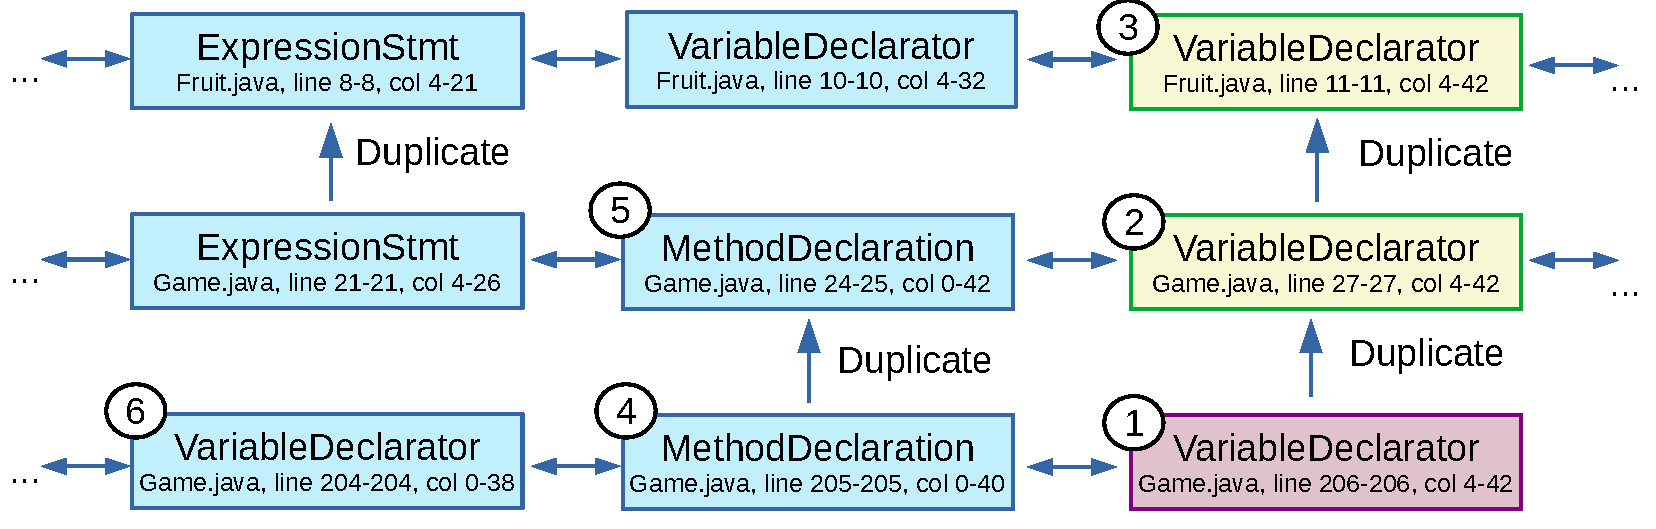
\includegraphics[width=1\columnwidth]{img/CodeGraphExample}
  \caption{Example of a clone graph built by CloneRefactor.}
  \label{fig:clonegraph2}
\end{figure}

Using the example shown in figure \ref{fig:clonegraph} and \ref{fig:clonegraph2} we can explain how we detect clones on basis of this graph. Suppose we are finding clones for two files and the final node of the second file is a variable declarator. This final node is represented in the example figure by the purple box (1). We then follow all ``duplicate'' relations until we have found all clones of this node (2 and 3). We now have a single statement clone class of three clone instances (1, 2 and 3).

Next, we move to the previous line (4). Here again, we collect all duplicates of this node (4 and 5). For each of these duplicates, we check whether the node following it is already in the clone class we collected in the previous iteration. In this case, (2) follows (5) and (1) follows (4). This means that node (3) does not form a `chain' with other cloned statements. Because of this, the clone class of (1, 2 and 3) comes to an end. It will be checked against the thresholds, and if adhering to the thresholds, considered a clone.

We then go further to the previous node (6). In this case, this node does not have any clones. This means we check the (2 and 5, 1 and 4) clone class against the thresholds, and if it adheres, consider it a clone. Dependent on the thresholds, this example can result in a total of two clone classes.

Eventually, following only the ``previous node'' relations, we can get from (6) to (2). When we are at that point, we will find only one cloned node for (2), namely (3). However, after we check this clone against the thresholds, we check whether it is a subset of any exisiting clone. If this is the case (which it is for this example), we discard the clone.

\subsubsection{Removing redundant clone classes}\label{sec:conceptualremovingredundant}
The clone detection method used by CloneRefactor can, for various reasons,%Should I list these? Listing them could be a section on its own, as I'd have to show examples to make it concrete.
result in redundant clone classes. After the insertion of each newly detected clone, we check whether it is redundant and/or any of the existent clones has become redundant by adding this clone. A clone is redundant if it is a subset of another clone. We define the subset relation between clones as follows:

\begin{equation}\label{eq:subset}
C_1 \subseteq C_2 := \forall (i_1 \in C_1) \text{ } \exists (i_2 \in C_2) \text{ } F i_1 = F i_2 \wedge R i_1 \subseteq R i_2
\end{equation} % Right symbol for definition

Where \textit{C} refers to a clone class (a set of clone instances), \textit{i} refers to a clone instance, \textit{F} is the file in which a clone instance is located and \textit{R} is the range of tokens that a clone instance spans. For each clone found, we remove all existing clones that are a subset of the found clone:

\begin{equation}\label{eq:removeall}
S_{after} = S_{before} \setminus \{C_{existing} \subseteq C_{new}\text{ }|\text{ }C_{existing} \in S_{before}\}
\end{equation}

Where \textit{$S_{before}$} is the clone class collection containing all clones that are found up in until this point and \textit{$C_{new}$} is the clone class that was just found. \textit{$S_{after}$} is the clone class collection after

We should not add the new clone to our list of clones if its a subset of an existing clone. Because of that, we check for each clone added whether there exists a clone class of which the found clone class is a subset:

\begin{equation}\label{eq:removeexisting}
\{C_{existing} \subseteq C_{new}\text{ }|\text{ }C_{existing} \in S\} = \emptyset \Rightarrow S_{after} = S \cup C_{new}
\end{equation}

If the newly added clone is a subset of an existing clone, we do not add it to the set of clone classes. This way we avoid redundant clone classes being detected by CloneRefactor.

\subsection{Validating the type 2R variability threshold}
In the definition of type 2R clones (see section \ref{sec:type2r}) we described how type 2R clones work on basis of a variability threshold. This threshold is checked by CloneRefactor to assess the validity of found clone classes. Implementing such a threshold involves some important design decisions and has a lot of underwater complexity. In this section we explain how CloneRefactor detects type 2R clones on basis of this variability threshold. This process is done as a postprocessing step after clone detection. The type 2R clone detection process is described in more detail in section \ref{sec:comparingstuff}. In short, this process detects clones allowing for any variability between expressions. This postprocessing step then determines which (parts of) these clones are valid by the configure variability threshold.

\begin{figure}[H]
  \centering
  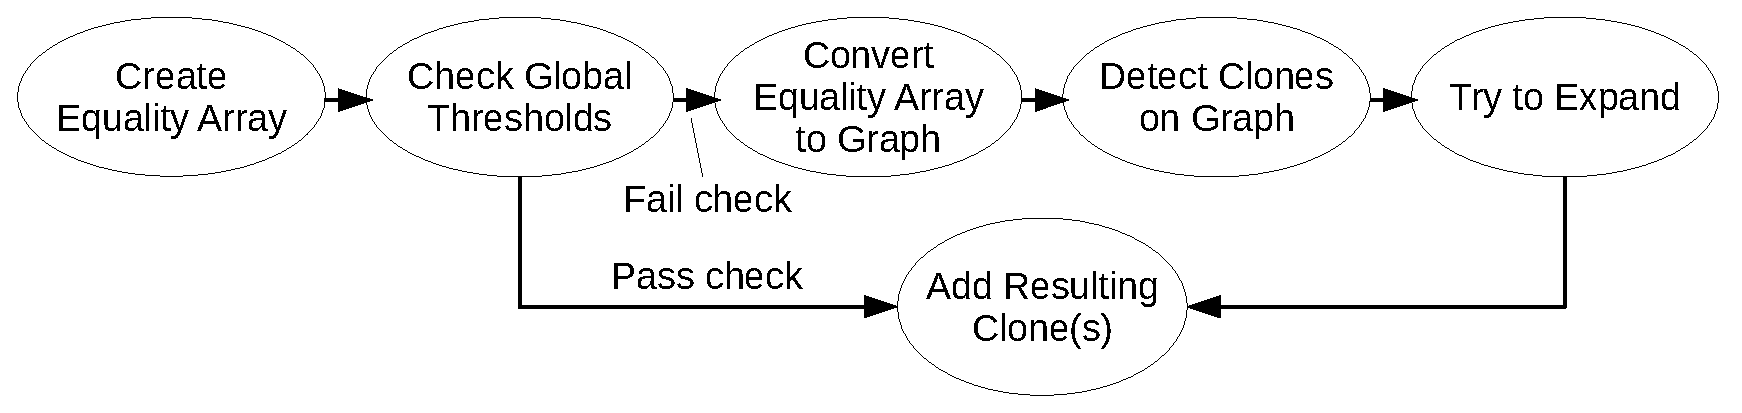
\includegraphics[width=1\columnwidth]{img/CloneRefactorT2RFlow}
  \caption{Process used to check the variability threshold for T2R clones.}
  \label{fig:clonerefactort2rflow}
\end{figure}

Figure \ref{fig:clonerefactort2rflow} shows the steps that CloneRefactor performs to find clones conforming with the type 2R variability threshold. Each of the following paragraphs will explain a step from this figure.

\subsubsection{Create equality array}
To determine the difference in literals, method calls and variables, we convert the code to an equality array. This equality array converts each (group of) token(s) to a number unique to that (group of) tokens. Each literal, method call or variable becomes a positive number, whereas each other token becomes a negative number. An example of two code fragments converted to equality arrays is displayed in figure \ref{fig:equalityarrays}.

\begin{figure}[H]
  \centering
  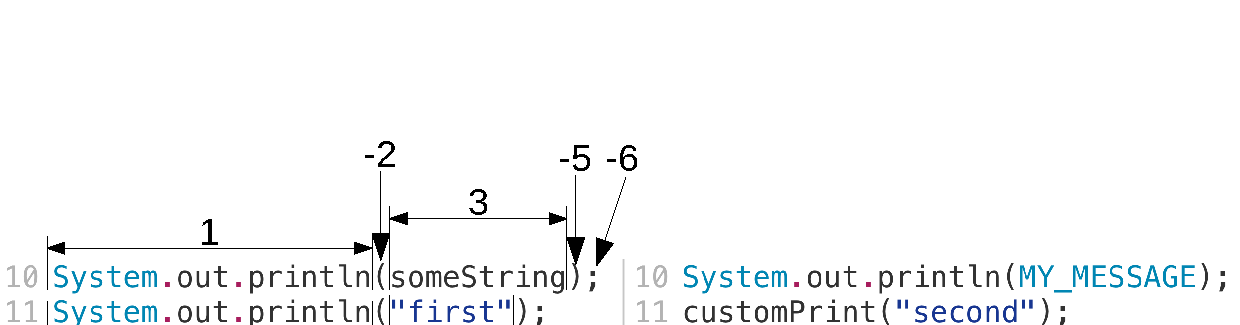
\includegraphics[width=1\columnwidth]{img/equality}
  \caption{The conversion of code to an equality array.}
  \label{fig:equalityarrays}
\end{figure}

The equality array for each of the lines in this example is shown in table \ref{table:equalityarrays}.

\begin{table}[H]
\begin{center}
 \caption{The equality arrays in our example figure \ref{fig:equalityarrays}.} \label{table:equalityarrays}
 \medskip
\begin{tabular}{|l|l|l|}
\hline
Node (n) & Equality Array (E) \\ \hline
1        & {[}1, -2, 3, -5, -6{]} \\ \hline
2        & {[}1, -2, 7, -5, -6{]} \\ \hline
3        & {[}1, -2, 4, -5, -6{]} \\ \hline
4        & {[}8, -2, 9, -5, -6{]} \\ \hline
\end{tabular}
\end{center}
\end{table}

In the example of figure \ref{fig:equalityarrays} the fragment on the left (consisting of $n_1$ and $n_2$) and the fragment on the right (consisting of $n_3$ and $n_4$) are two clone instances of a clone class. Table \ref{table:equalityarrays} shows their corresponding equality arrays.

\subsubsection{Checking global thresholds} \label{sec:t2rcheckglobalthres}
Using the equality arrays explained in the previous section, we can determine the variability threshold of any clone class. We calculate the variability of the example given in table \ref{table:equalityarrays} as follows:

\begin{equation}\label{eq:variabilityclonerefactor}
\text{T2R Variability} = \frac{|\{x>0 \land y>0 \land x \neq y \Rightarrow (x,y) \text{ }|\text{ }x \in E_1 \cup E_2, y \in E_3 \cup E_4\}|}{|\{x>0 \land y>0 \Rightarrow (x,y) \text{ }|\text{ }x \in E_1 \cup E_2, y \in E_3 \cup E_4\}|}*100
\end{equation}

Where $E_x$ refers to the equality arrays shown in table \ref{table:equalityarrays} and \textit{x} is the node number displayed in the same table. When we apply this equation to the example clone classes displayed in figure \ref{fig:equalityarrays}, we get the following sum:

\begin{equation}\label{eq:sumequality}
\frac{|\{(3,4), (1,8), (7,9)\}|}{|\{(1,1), (3,4), (1,8), (7,9)\}|}*100 = \frac{3}{4}*100 = 75\%
\end{equation}

So for the example given in figure \ref{fig:equalityarrays} we have a variability of 75r \%. In CloneRefactor, the maximum variability percentage is a threshold that is entered in a configuration file. If a clone adheres to this threshold, it will stay in the set of found clones. However, if it does not adhere to the thresholds, a problem arises. Because a clone does not adhere to the thresholds, it does not yet mean it has to be discarded. This is because an invalid clone class can still contain valid clones that are a subset of the invalid clone (our definition of subsets of clones is given in section \ref{sec:conceptualremovingredundant}).

%Two nodes are considered clones of each other if the size of their equality array is equal and all negative numbers in the equality array are equal.


When a found clone class does not adhere to the global thresholds as explained in the previous section, we need to determine whether it contains any valid subclones. Below, we explain a few cases of valid subclones that may exist within an invalid clone class.

\begin{figure}[H]
\begin{parcolumns}{2}
\colchunk[1]{
\begin{javacode}
doA(a, b, c);
|\highlightYellow|doA();
|\highlightYellow|doB();
|\highlightYellow|doC();
\end{javacode}}
\colchunk[2]{
\begin{javacode}
doB(d, e, f);
|\highlightYellow|doA();
|\highlightYellow|doB();
|\highlightYellow|doC();
\end{javacode}}
\end{parcolumns}
\caption{One node in a type 2R clone has a high variability.}
\label{fig:2rvariabilityhigh1}
\end{figure}

The first line of the cloned fragment shown in figure \ref{fig:2rvariabilityhigh1} has a high variability with its cloned fragement. However, the rest of this method does not have any variability. The global thresholds could indicate a too high variability and thus render this clone invalid. However, in this case, it might still have a valid subclone.

\begin{figure}[H]
\begin{parcolumns}{3}
\colchunk[1]{
\begin{javacode}
|\highlightYellow|doA();
|\highlightYellow|doB();
|\highlightYellow|doC();
\end{javacode}}
\colchunk[2]{
\begin{javacode}
|\highlightYellow|doA();
|\highlightYellow|doB();
|\highlightYellow|doC();
\end{javacode}}
\colchunk[3]{
\begin{javacode}
doD();
doE();
doF();
\end{javacode}}
\end{parcolumns}
\caption{One clone instance in a type 2R clone has a high variability.}
\label{fig:2rvariabilityhigh2}
\end{figure}

Another example of high variability between clones, in which a valid subclone can be found, is displayed in figure \ref{fig:2rvariabilityhigh2}. In this case, one clone instance has such a high variability that it shouldn't be refactored. In this case, the clone instance with high variability should be removed.

\begin{figure}[H]
\begin{parcolumns}{3}
\colchunk[1]{
\begin{javacode}
|\highlightYellow|doA();
|\highlightYellow|doB();
doC();
doC();
\end{javacode}}
\colchunk[2]{
\begin{javacode}
doD();
|\highlightYellow|doA();
|\highlightYellow|doB();
doD();
\end{javacode}}
\colchunk[3]{
\begin{javacode}
doE();
doE();
|\highlightYellow|doA();
|\highlightYellow|doB();
\end{javacode}}
\end{parcolumns}
\caption{A small subset of nodes has a high variability.}
\label{fig:2rvariabilityhigh3}
\end{figure}

Figure \ref{fig:2rvariabilityhigh3} shows an example of a clone class where the valid sequence inside the clone does not align.

If the check for global thresholds fails, we have to seek for valid clones within the clone class. In a single invalid clone class can be zero to many subclones. This requires an extensive search for such clones. This problem is very related to the problem of clone detection, except now it is within the boundaries of a single clone class except for an entire codebase. Because of that, just like the clone detection process, we build a clone graph and detect clones on it. This process is explained over the following sections.

\subsubsection{Convert Equality Array to Graph}
After the global threshold check has failed, we build a clone graph on basis of the equality arrays. The process used for building this graph is the same as the process described in \ref{sec:buildingclonegraph}.

\begin{figure}[H]
\begin{parcolumns}{3}
\colchunk[1]{
\begin{javacode}
|\highlightYellow|doA(); //{1, -2}
|\highlightYellow|doB(); //{3, -2}
doC(); //{4, -2}
doC(); //{4, -2}
\end{javacode}}
\colchunk[2]{
\begin{javacode}
doD(); //{5, -2}
|\highlightYellow|doA(); //{1, -2}
|\highlightYellow|doB(); //{3, -2}
doD(); //{5, -2}
\end{javacode}}
\colchunk[3]{
\begin{javacode}
doE(); //{6, -2}
doE(); //{6, -2}
|\highlightYellow|doA(); //{1, -2}
|\highlightYellow|doB(); //{3, -2}
\end{javacode}}
\end{parcolumns}
\caption{Cloned code fragments from figure \ref{fig:2rvariabilityhigh3} together with their equality arrays.}
\label{fig:2rvariabilityhigh4}
\end{figure}

In figure \ref{fig:2rvariabilityhigh4} we display clone classes and their (simplified) equality arrays. We can convert this to a graph, using a similar process as the graph creation process used for clone detection. In this case, duplicate relations represent nodes of which their equality arrays are within the variability threshold. In figure \ref{fig:2rvariabilityhigh4} all relations are between equal equality arrays, but this does not always have to be the case. Large equality arrays, denoting statements that consist of many tokens, may have some variability and still be considered duplicates in this graph.

\begin{figure}[H]
  \centering
  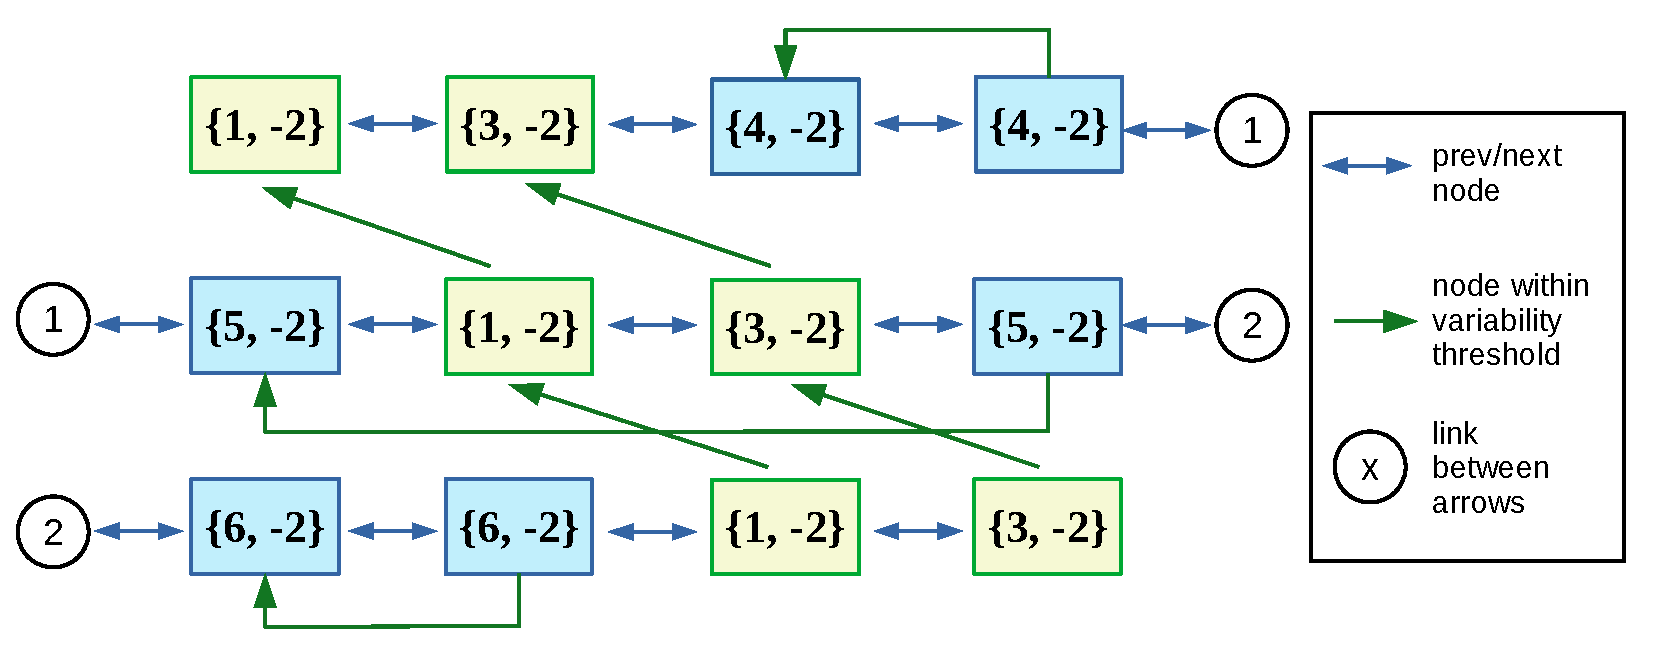
\includegraphics[width=1\columnwidth]{img/T2RGraph}
  \caption{Graph representation of the code example displayed in figure \ref{fig:2rvariabilityhigh4}.}
  \label{fig:clonerefactorprocess}
\end{figure}

In this graph, the duplicate relations (green arrows) do not necessarily denote an exact match. The duplicate relations allow for variability in the equality arrays as long as it falls under the variability threshold. However, negative numbers in the equality array may never vary. This is because negative numbers are the tokens/expressions that we do not allow variability in because they cannot be refactored as easily:
\begin{equation}\label{eq:t2rcloneequality}
E_1\text{ can only be cloned with }E_2\text{ iff }|E_1|=|E_2| \land \forall (x \in E_1, y \in E_2)\text{ }x<0 \lor y<0 \Rightarrow x=y
\end{equation}

\subsubsection{Detect Clones on Graph}
Similar to the clone detection process, we detect clones on basis of the graph described in the previous section. The only difference is that, in this step, we do not remove clones that do not meet the thresholds (as explained in section \ref{sec:clonerefactorthresholds}). This is because the next step, explained in the next section, could potentially expand the found clones and thus make clones that would currently invalid by the thresholds valid.

Looking back at the example of the previous section, it would result in the following clone class collection:
\begin{figure}[H]
\begin{parcolumns}{3}
\colchunk[1]{
\begin{javacode}
|\highlightYellow|doA(); // |\textcolor{pgreen}{$C_1$ $I_3$}|
|\highlightYellow|doB(); // |\textcolor{pgreen}{$C_1$ $I_3$}|
doC(); // |\textcolor{pgreen}{$C_4$ $I_2$}|
doC(); // |\textcolor{pgreen}{$C_4$ $I_1$}|
\end{javacode}}
\colchunk[2]{
\begin{javacode}
doD(); // |\textcolor{pgreen}{$C_3$ $I_2$}|
|\highlightYellow|doA(); // |\textcolor{pgreen}{$C_1$ $I_2$}|
|\highlightYellow|doB(); // |\textcolor{pgreen}{$C_1$ $I_2$}|
doD(); // |\textcolor{pgreen}{$C_3$ $I_1$}|
\end{javacode}}
\colchunk[3]{
\begin{javacode}
doE(); // |\textcolor{pgreen}{$C_2$ $I_2$}|
doE(); // |\textcolor{pgreen}{$C_2$ $I_1$}|
|\highlightYellow|doA(); // |\textcolor{pgreen}{$C_1$ $I_1$}|
|\highlightYellow|doB(); // |\textcolor{pgreen}{$C_1$ $I_1$}|
\end{javacode}}
\end{parcolumns}
\caption{Clone instances in figure \ref{fig:2rvariabilityhigh4} as determined .}
\label{fig:2rvariabilityhigh5}
\end{figure}

Where \textit{C} denotes the clone class and \textit{I} denotes the clone instance. The process by which these clones are found is equal to the clone detection process as described in section \ref{sec:detectingclones}. In this example, we see the four clones found on the graph of figure \ref{fig:clonerefactorprocess}. Three of these clone classes have a two clone instances, each consisting of a single nodes. The other clone class has three clone instances, each consisting of two nodes.

\subsubsection{Try to Expand}
The problem with the graph clone detection technique is that only single nodes that are within the variability threshold are considered duplicates of each other. However, single nodes that are not within this threshold could still be part of a clone class if the other cloned nodes are more towards the lower bound of the threshold.

\begin{figure}[H]
\begin{parcolumns}{2}
\colchunk[1]{
\begin{javacode}
|\highlightYellow|doA(a); //{1, -2, 7, -3, -4}
doB(a); //{5, -2, 7, -3, -4}
|\highlightYellow|doD(); //{8, -2, -3, -4}
|\highlightYellow|doE(); //{9, -2, -3, -4}
|\highlightYellow|doF(); //{10, -2, -3, -4}
doG(a); //{11, -2, 7, -3, -4}
\end{javacode}}
\colchunk[2]{
\begin{javacode}
|\highlightYellow|doA(a); //{1, -2, 7, -3, -4}
doC(a); //{6, -2, 7, -3, -4}
|\highlightYellow|doD(); //{8, -2, -3, -4}
|\highlightYellow|doE(); //{9, -2, -3, -4}
|\highlightYellow|doF(); //{10, -2, -3, -4}
doH(b); //{12, -2, 13, -3, -4}
\end{javacode}}
\end{parcolumns}
\caption{Type 2R clones with their equality arrays.}
\label{fig:trytoexpand}
\end{figure}

As an example, consider the clone fragment in figure \ref{fig:trytoexpand}. In this example, we have 2 clone classes. In the ``Try To Expand'' step, we will check whether we can create a clone class with larger clone instances on basis of the clones found in the previous step. We start with the largest clone class, measured in clone volume. We measure clone volume as the product of the amount of clone instances in a clone class and the amount of nodes in any of its instances.

In the example in figure \ref{fig:trytoexpand} the largest instance has a volume of:

\begin{equation}\label{eq:clonevolume}
3 \text{ nodes} * 2 \text{ clone instances} = 6
\end{equation}

Starting from this clone, we will try to expand it. We will include the previous node in the clone class and verify its variability threshold (node $N_2$). In this case, using the formulas shown in section \ref{sec:t2rcheckglobalthres}, we can check whether this clone class would be valid by the variability threshold:

\begin{equation}\label{eq:variabilitycombined1}
\frac{|\{(5,6)\}|}{|\{(5,6),(7,7),(8,8),(9,9),(10,10)\}|}*100 = \frac{1}{5}*100 = 20\%
\end{equation}

Dependent on the actual variability threshold, the clone class would get expanded with node $N_2$. For this example, we assume the variability threshold is set to 15\%. In such a case, including this node would not result in a valid clone class. However, we continue trying to expand this clone class until we have reached the first node of the originally cloned fragment (the cloned fragment that did not take the variability threshold into account). Thus, we now try to expand with $\{N_1, N_2\}$. We then get the following formula:

\begin{equation}\label{eq:variabilitycombined2}
\frac{|\{(5,6)\}|}{|\{(1,1),(7,7),(5,6),(7,7),(8,8),(9,9),(10,10)\}|}*100 = \frac{1}{7}*100 = 14\%
\end{equation}

This falls under the threshold of 15\% so we expand the clone class. Thus, the clone class $\{N_3, N_4, N_5\}$ will become $\{N_1, N_2, N_3, N_4, N_5\}$. We cannot expand further because we have reached the end of the original cloned fragment. When we are done expanding to previous nodes, we will try to expand to next nodes. In this case, we check whether we can include $N_6$ into the clone class. If $N_6$ would be included, the variability threshold would be as follows:

\begin{equation}\label{eq:variabilitycombined3}
\frac{|\{(5,6),(11,12),(7,13)\}|}{|\{(1,1),(7,7),(5,6),(7,7),(8,8),(9,9),(10,10),(11,12),(7,13)\}|}*100 = \frac{3}{9}*100 = 33\%
\end{equation}

This does not fall within the variability threshold, so we do not include this node in the clone class. After we have checked a single clone class within the bigger cloned fragment for expansion opportunities, we go on with the next clone class (by volume). In this case, the other clone class within this fragment has become a subset of the clone class we just expanded. Because of that, this other clone class is discarded. For the example code fragment in figure \ref{fig:trytoexpand} the resulting clone class is $\{N_1, N_2, N_3, N_4, N_5\}$.

\subsection{Checking for type 3 opportunities} \label{sec:t3rclonerefactor}
As described in section \ref{sec:type3r}, we define type 3R clones as gapped clones. This means that two existing clones may have a gap of non-gapped clones. We check for every found clone class whether it is a type 3R clone with another clone:

\begin{equation}\label{eq:crtype3r}
\forall (c_1 \in S) \text{ }\exists (c_2 \in S)\text{ }x \neq y \land isType3R(c_1, c_2)
\end{equation}

Where \textit{S} is the set of all found clone classes. $\text{isType3R}(C_1, C_2)$ is a Boolean-valued function that returns whether two clone classes are type 3R clones of each other. Two clone classes are type 3R clones of each other if each of their instances are within a certain distance of each other:

\begin{equation}\label{eq:istype3r}
\text{isType3R}(C_1, C_2) = \forall (i_1 \in C_1)\text{ } \exists (i_2 \in C_2)\text{ } Fi_1 = Fi_2 \land gap(i_1, i_2) < gap\_threshold
\end{equation}

Where \textit{F} is the file in which the clone instance is located. \textit{gap\_threshold} is the defined threshold percentage of the maximum gap size between two clone instances. $\text{gap}(I_1, I_2)$ is the function that calculates the gap between two clone instances. This gap is calculated by dividing the amount of statements in the gap by the amount of statements that both clone instances span together:

\begin{equation}\label{eq:t3rgap}
\text{gap}(i_1, i_2) = \frac{|\{(Rn>Ri_1 \land Rn<Ri_2) \lor (Rn>Ri_2 \land Rn<Ri_1)\text{ }|\text{ } n \in nodes(Fi_1)\}|}{|i_1| + |i_2|} * 100
\end{equation}

Where \textit{F} is the file in which the clone instance is located and \textit{R} is the range of a clone instance or node. A range denotes the line and column at which a code fragment starts and ends. We define the partial order relationship on ranges as follows:

\begin{equation}\label{eq:rangetotalorder}
r_1 < r_2 \text{ iff } ELr_1 < BLr_2 \lor (ELr_1 = BLr_2 \land ECr_1 < BCr_2)
\end{equation}
\begin{equation}\label{eq:rangetotalorder2}
r_1 > r_2 \text{ iff } BLr_1 > ELr_2 \lor (BLr_1 = ELr_2 \land BCr_1 > ECr_2)
\end{equation}

Where \textit{BL} is the begin line of a range, \textit{EL} is the end line of a range, \textit{BC} is the begin column of a range and \textit{EC} is the end column of a range.

\subsubsection{Example}
In this section we show an example of the identification of a type 3R clone.

\begin{figure}[H]
\begin{parcolumns}{2}
\colchunk[1]{
\begin{javacode}
//File1.java
|\highlightYellow|doA(); // |\textcolor{pgreen}{$C_1$ $I_1$}|
|\highlightYellow|doB(); // |\textcolor{pgreen}{$C_1$ $I_1$}|
doC();
|\highlightBlue|doC(); // |\textcolor{pgreen}{$C_2$ $I_1$}|
|\highlightBlue|doD(); // |\textcolor{pgreen}{$C_2$ $I_1$}|
\end{javacode}}
\colchunk[2]{
\begin{javacode}
//File2.java
|\highlightYellow|doA(); // |\textcolor{pgreen}{$C_1$ $I_2$}|
|\highlightYellow|doB(); // |\textcolor{pgreen}{$C_1$ $I_2$}|
|\highlightBlue|doC(); // |\textcolor{pgreen}{$C_2$ $I_2$}|
|\highlightBlue|doD(); // |\textcolor{pgreen}{$C_2$ $I_2$}|
\end{javacode}}
\end{parcolumns}
\caption{Gapped clones.}
\label{fig:3ropportunities}
\end{figure}

In the example of figure \ref{fig:3ropportunities} we see two clone classes, which are separated by a single node. Using equation \ref{eq:t3rgap} we can calculate the size of the gap as follows:

\begin{equation}\label{eq:t3rexample}
\text{gap}(C_1\text{ }I_1, C_2\text{ }I_1) = \frac{|\{n_4\}|}{|\{n_2, n_3\}| + |\{n_5, n_6\}|} * 100 = \frac{1}{4} = 25\%
\end{equation}

The same calculation is conducted for the other clone instances:

\begin{equation}\label{eq:t3rexample}
\text{gap}(C_1\text{ }I_2, C_2\text{ }I_2) = \frac{|\emptyset|}{|\{n_2, n_3\}| + |\{n_4, n_5\}|} * 100 = \frac{0}{4} = 0\%
\end{equation}

If all resulting percentages are under the threshold, this clone will be added to the collection of found clones and all of its subsets will be removed.

\section{Context Analysis of Clones}\label{chap:contextsetup}
To be able to refactor code clones, CloneRefactor first maps the context of code clones. We define the following aspects of the clone as its context:
\begin{enumerate}
  \item \textbf{Relation:} The relation of clone instances among each other through inheritance.
  \item \textbf{Location:} Where a clone instance occurs in the code.
  \item \textbf{Contents:} The statements/declarations of a clone instance.
\end{enumerate}
We define categories for each of these aspects and enable CloneRefactor to determine the categories of clones.

\begin{figure}[H]
  \centering
    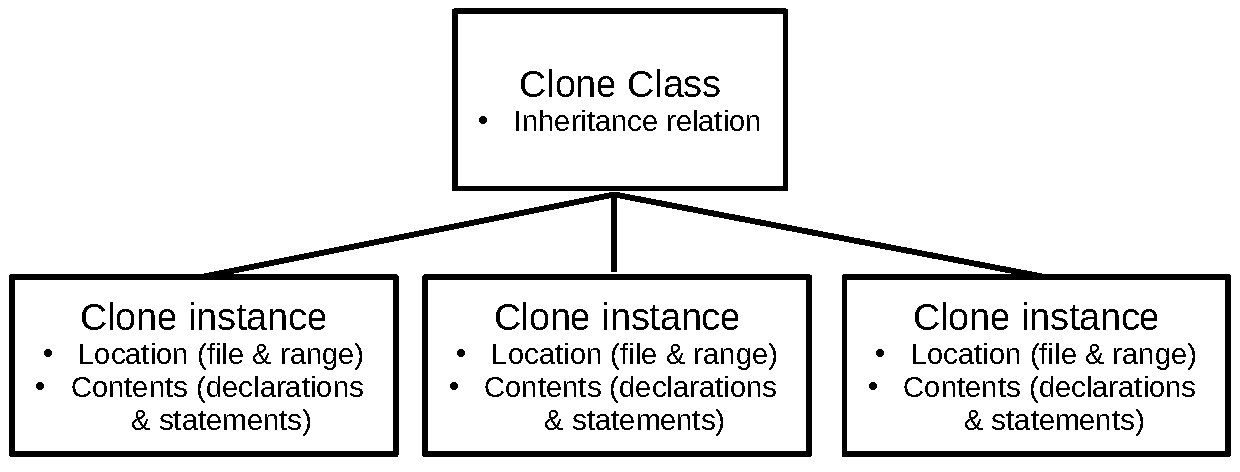
\includegraphics[width=0.8\columnwidth]{img/context}
    \caption{Abstract representation of clone classes and clone instances.}
  \label{fig:clonecontext}
\end{figure}

Fig.~\ref{fig:clonecontext} shows an abstract representation of clone classes and clone instances. The relation of clones through inheritance is measured for each clone class. The location and contents of clones are measured for each clone instance.

\subsection{Relation}\label{sec:setuprelation}
When merging code clones in object-oriented languages, it is important to consider the inheritance relation between clone instances. This relation has a big impact on how a clone should be refactored.

Fontana et al.~\cite{fontana2015duplicated} describe measurements on 50 open source projects on the relation of clone instances to each other. To do this, they first define several categories for the relation between clone instances in object-oriented languages. These categories are as follows:
\begin{enumerate}
  \item \textbf{Same Method}: All instances of the clone class are in the same method.
  \item \textbf{Same Class}: All instances of the clone class are in the same class.
  \item \textbf{Superclass}: All instances of the clone class are in a class that is child or parent of each other.
  \item \textbf{Sibling Class}: All instances of the clone class have the same parent class.
    \item \textbf{Ancestor Class}: All instances of the clone class are superclasses except for the direct superclass.
  \item \textbf{First Cousin Class}: All instances of the clone class have the same grandparent class.
\item \textbf{Same Hierarchy Class}: All instances of the clone class belong to the same inheritance hierarchy, but do not belong to any of the other categories.
\item \textbf{Same External Superclass}: All instances of the clone class have the same superclass, but this superclass is not included in the project but part of a library.
\item \textbf{Unrelated class}: There is at least one instance in the clone class that is not in the same hierarchy.
\end{enumerate}

We added the following categories, to gain more information about clones and reduce the number of unrelated clones:

\begin{enumerate}
\item \textbf{Same Interface}: All instances of the clone class are in a class or interface that have a common interface anywhere in their inheritance hierarchy.
\item \textbf{No Direct Superclass}: All instances of the clone class are in a class that does not have any superclass.
\item \textbf{No Indirect Superclass}: All instances of the clone class are in a class that does not have any external classes in its inheritance hierarchy.
\item \textbf{External Ancestor}: All instances of the clone class are in a class that does not have any external classes in its inheritance hierarchy.
\end{enumerate}

Figure \ref{fig:clonecontext} shows an abstract representation of clone classes and clone instances. The relation of clones through inheritance is measured on clone class level: it involves all child clone instances. The location and contents of clones is measured on clone instance level. A clone's location involves the file it resides in and the range it spans (for example: line 6 col 2 - line 7 col 50). A clone instance contents consists of a list of all statements and declarations it spans.

\begin{figure}[H]
  \centering
    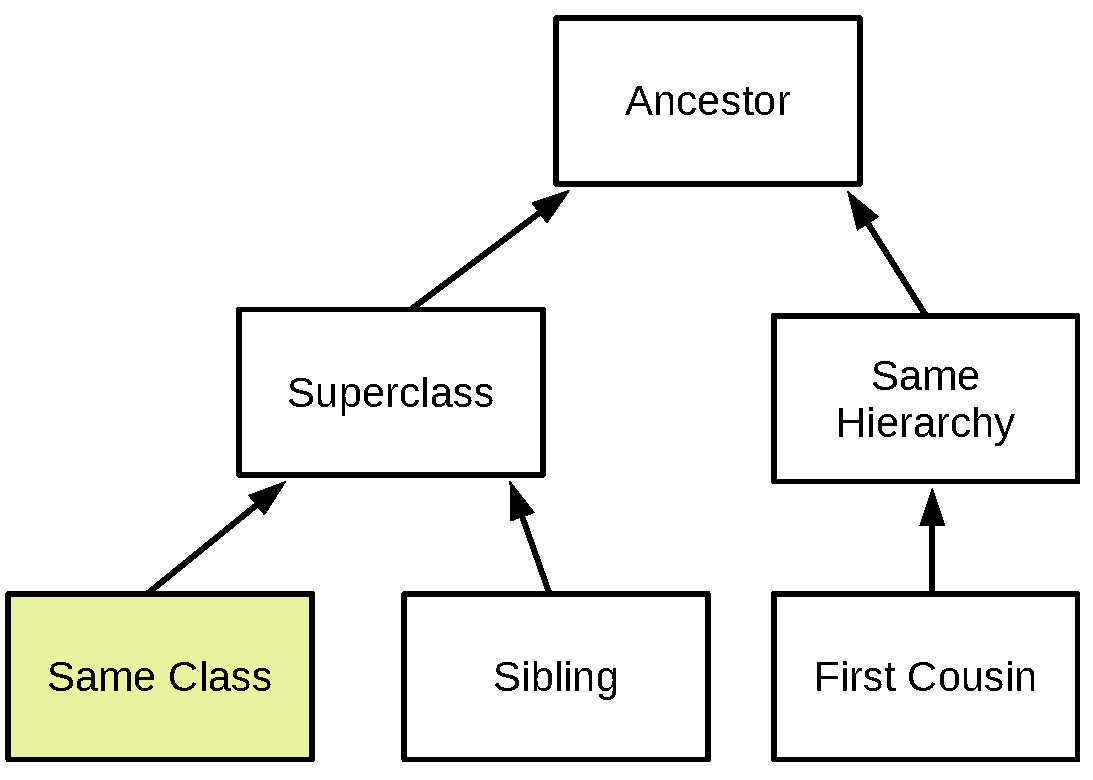
\includegraphics[width=0.6\columnwidth]{img/Relation}
      \caption{Abstract figure displaying relations of clone classes. Arrows represent superclass relations.}
  \label{fig:clonerelation}
\end{figure}

We separate these relations into the following categories, because of their related refactoring opportunities:
\begin{itemize}
  \item \textbf{Common Class}: \textit{Same Method}, \textit{Same Class}
  \item \textbf{Common Hierarchy}: \textit{Superclass}, \textit{Sibling Class}, \textit{Ancestor Class}, \textit{First Cousin}, \textit{Same Hierarchy}
  \item \textbf{Common Interface}: \textit{Same Interface}
  \item \textbf{Unrelated}: \textit{No Direct Superclass}, \textit{No Indirect Superclass}, \textit{External Superclass}, \textit{External Ancestor}
\end{itemize}

Every clone class only has a single relation, which is the first relation from above list that the clone class applies to. For instance: all ``Superclass'' clones also apply to ``Same Hierarchy'', but because ``Superclass'' is earlier in above list they will get the ``Superclass'' relation. This is because the items earlier in the list denote a more favorable refactoring.

To check a the relation for a given clone class, we compare each node in a clone instance with the respective nodes in each other clone instance within a clone class. So for a clone class with x clone instances and each clone instance has y nodes, we perform:

\begin{equation}\label{eq:sameclass}
\frac{x * (x + 1)}{2} * y
\end{equation}

comparisons to determine the relation. Each of these checks will result in one of the relations from the list above. Of these relations, the item lowest in the list is going to be the relation of the clone class. So for instance, if a clone class has 15 nodes that denote a \textit{Superclass} relation but 3 nodes are \textit{Unrelated}, the clone class becomes \textit{Unrelated}.

\subsubsection{Common Class}
The \textit{Same method} and \textit{Same class} relations share a common refactoring opportunity. Clones of both these categories, when extracted to a new method, can be placed in the same class. Both of these relations are most favorable for refactoring, as they require a minimal design tradeoff. Furthermore, global variables that are used in the class can be used without having to create method parameters.

Cloned nodes are flagged as \textit{Same method} if these nodes are found in the same method. We define the method as the first method declaration that is encountered when following the parent nodes in the ast for a given cloned node. Please note that a clone instance may not always be in a method, for which this predicate will fail.

Cloned nodes are flagged as \textit{Same class} if these nodes are found in the same class. We define the class as the first class declaration that is encountered when following the parent nodes in the ast for a given cloned node.

\subsubsection{Common Hierarchy}
Clones that are in a common hierarchy can be refactored by using the ``Extract Method'' refactoring method followed by ``Pull Up Method'' until the method reaches a location that is accessible by all clone instances. However, the more often ``Pull Up Method'' has to be used, the more detrimental the effect is on system design. This is because putting a lot of functionality in classes higher up in an inheritance structure can result in the ``God Object'' anti-pattern. A god object is an object that knows too much or does too much.

Cloned nodes are flagged as \textit{Superclass} if the classes in which these nodes are found are parent and child class of each other. Cloned nodes are flagged as \textit{Siblings} if the classes in which these nodes are found all share the same parent and this parent class is not external. Cloned nodes are flagged as \textit{First Cousin} if the classes in which these nodes are found all share the same grandparent and this grandparent class is not external.

Cloned nodes are flagged as \textit{Ancestor} if the classes in which these nodes are found are recursively the parent of an antecedent. Cloned nodes are flagged as \textit{Same Hierarchy} if the classes in which these nodes are found are all in the same inheritance hierarchy and not linked by any external classes.

\subsubsection{Common Interface}
Many object-oriented languages know the concept of ``interfaces'', which are used to specify a behavior that classes must implement. As code clones describe functionality and interfaces originally did not allow for functionality, interfaces did not open up refactoring opportunities for duplicated code. However, many programming languages nowadays support default implementations in interfaces. Since Java 7 and C\#8, these programming languages allow for functionality to be defined in interfaces. Many other object-oriented languages like Python allow this by nature, as they do not have a true notion of interfaces.

The greatest downside on system design of putting functionality in interfaces is that interfaces are per definition part of a classes' public contract. That is, all functionality that is shared between classes via an interface cannot be hidden by setting a stricter visibility. Because of that, we favor all ``Common Hierarchy'' refactoring opportunities over ``Common Interface''.

To check whether two cloned nodes have common interfaces, we recursively walk all types the class or interface of the cloned nodes implement and extend. The common interface that is closest to the cloned node in terms of depth of recursion will be flagged as the refactoring candidate.

\subsubsection{Unrelated}
Clones are unrelated if they share no common class or interface in their inheritance structure. These clones are least favorable when looking at refactoring, because their refactoring will almost always have a major impact on system design. We formulated four categories of unrelated clones to look into their refactoring opportunities.

Cloned nodes are flagged \textit{No Direct Superclass} if they are in classes that do currently not have a parent. This marks the opportunity for creating a superclass abstraction and placing the extracted method there. Cloned nodes are flagged \textit{No Indirect Superclass} if any of their ancestors does not have a parent. In such a case, it would be possible to create such an abstraction for the ancestor that does not have a parent.

Cloned nodes are flagged \textit{External Superclass} if they are in a class which has an external parent. Cloned nodes are flagged \textit{External Ancestor} if one of their ancestors has an external parent. Both of these relations obstruct the possibility of creating a superclass abstraction. In such a case, an interface abstraction could be created to make their relation explicit.

\subsection{Location}\label{sec:setuplocation}
A paper by Lozano et al. \cite{lozano2007evaluating} discusses the harmfulness of cloning. The authors argue that 98\% are produced at method-level. However, this claim is based on a small dataset and based on human copy-paste behavior rather than static code analysis. We decided to measure the locations of clones through static analysis on our dataset. We chose the following categories:
\begin{enumerate}
  \item \textbf{Method/Constructor Level:} A clone instance that does not exceed the boundaries of a single method or constructor (optionally including the declaration of the method or constructor itself).
  \item \textbf{Class Level:} A clone instance in a class, that exceeds the boundaries of a single method or contains something else in the class (like field declarations, other methods, etc.).
  \item \textbf{Interface Level:} A clone that is (a part of) an interface.
  \item \textbf{Enumeration Level:} A clone that is (a part of) an enumeration.
\end{enumerate}
We check the location of each clone instance for each of its nodes. If any node reports a different location from the others, we choose the location that is lowest in above list. So for instance, if a clone instance has 15 nodes that denote a \textit{Method Level} location but 3 nodes are \textit{Class Level}, the clone instance becomes \textit{Class Level}.

\subsubsection{Method/Constructor Level Clones} \label{sec:methodlevelcr}
Method/Constructor Level clones denote clones that span are found in either a method or contructor. A constructor is a special method that is called when an object is instantiated. Current clone refactoring studies only focus on clones at method level \cite{choi2011extracting, yue2018automatic, kodhai2013method, arcelli2013software, lin2014clonepedia, mandal2014automatic, balazinska2000advanced, yongting2018detection, bouktif2006novel, fanqi2014using, devi2016study}. This is because most clones reside at those places \cite{lozano2007evaluating, fontana2015duplicated} and most of those clones can be refactored with a relatively simple set of refactoring techniques \cite{kodhai2013method, fontana2015duplicated}.

To detect whether a given clone instance is at Method Level, we check for each node in the clone instance whether it has an ancestor node that is a method declaration. A clone instance is considered ``Method Level'' if:

\begin{equation}\label{eq:samemethod}
\forall (n \in I)\text{ } Tn = \text{MethodDeclaration} \lor \exists (p \in ancestors(n)) \text{ } Tp = \text{MethodDeclaration}
\end{equation}

Where \textit{T} is the type of a node. \textit{ancestors(n)} denotes all of ancestor nodes of a node. The ancestor nodes are recursively all the parents of a given node in the AST. Apart from this, we check that the MethodDeclaration ancestor of each clone instance is the same, to be sure the clone only spans a \textit{single} method. Figure \ref{fig:methodlevelclone} shows an example of a method level clone and its recursive parents.

\begin{figure}[H]
\begin{parcolumns}{2}
\colchunk[1]{
\begin{javacode}
public class Class1 { // |\textcolor{pgreen}{$p_3$}|
  public void doA() { // |\textcolor{pgreen}{$p_2$}|
    if(isA()) // |\textcolor{pgreen}{$p_1$}|
|\highlightYellow|      doB(); // |\textcolor{pgreen}{$n_1$}|
  }
}
\end{javacode}}
\colchunk[2]{
\begin{javacode}
\begin{javacode}
public class Class2 { // |\textcolor{pgreen}{$p_3$}|
  public void doB() { // |\textcolor{pgreen}{$p_2$}|
    if(isB()) // |\textcolor{pgreen}{$p_1$}|
|\highlightYellow|      doB(); // |\textcolor{pgreen}{$n_2$}|
  }
}
\end{javacode}}
\end{parcolumns}
\caption{Example of a method level clone and its parents.}
\label{fig:methodlevelclone}
\end{figure}

\subsubsection{Class/Interface/Enumeration Level Clones}
Class/Interface/Enumeration Level clone instances are found inside the body of one of these declarations and optionally include the declaration itself. It can also be a clone instance that exceeds the boundaries of a single method. These clone instances can contain a fields, (abstract) methods, inner classes, enumeration fields, etc. These types of clones require various refactoring techniques to refactor. For instance, we might have to move fields in a inheritance hierarchy. Or, we might have to perform a refactoring on more of an architectural level, if a large set of methods is cloned.

We detect these clones in the same way we detect method level clones: we walk up the AST until we find the first node that indicates one of these categories.

\subsection{Contents}\label{sec:setupcontents}
Finally, we looked at what nodes individual clone instances span. We selected the following categories to be relevant for refactoring:
\begin{enumerate}
  \item \textbf{Full Method/Class/Interface/Enumeration:} A clone that spans a full class, method, constructor, interface or enumeration, including its declaration.
  \item \textbf{Partial Method/Constructor:} A clone that spans (a part of) the body of a method. The declaration itself is not included.
  \item \textbf{Several Methods:} A clone that spans over two or more methods, either fully or partially, but does not span anything but methods (so not fields or anything in between).
  \item \textbf{Only Fields:} A clone that spans only global variables.
  \item \textbf{Includes Fields/Constructor:} A clone that spans a combination of fields and other things, like methods.
  \item \textbf{Method/Class/Interface/Enumeration Declaration:} A clone that contains the declaration (usually the first line) of a class, method, interface or enumeration.
  \item \textbf{Other:} Anything that does not match with above-stated categories.
\end{enumerate}

\subsubsection{Full Method/Class/Interface/Enumeration}
These categories denote that a full declaration, including its body, is cloned with another declaration. These categories often denote redundancy and are often easy to solve: one of both declarations is redundant and should be removed. All usages of the removed declaration should be redirected to the clone instance that was not removed. We check for clones in this category by checking that the first node in a clone instance is a declaration and the last node in the clone instance is the last node in the body of that declaration.

\subsubsection{Partial Method/Constructor}
These categories describe clone instances which are found in the body of a method or constructor. These clones can often be refactored by extracting a new method out of the cloned code. We detect such clones by checking that each node in the clone instance has a parent node that is a methoddeclaration, but none of the nodes is a method declaration. We describe the procedure by with we recursively seek the parent nodes of a node in section \ref{sec:methodlevelcr}.

\subsubsection{Several Methods}
Several methods cloned in a single class is a strong indication of implicit dependencies between two classes. This increases the chance that these classes are missing some form of abstraction, or their abstraction is used inadequately. We detect such clones by checking that each cloned node has a parent node that is a MethodDeclaration. This is the same process as described in equation \ref{eq:samemethod}. Additionally, we check that the MethodDeclaration ancestor of the first node in the clone instance differs from the last, to be sure that the clone instance spans over at least two methods.

\subsubsection{Only Fields}
This category denotes that the clone spans over only global variables, fields that are declared outside of a method. This is to indicate data redundancy: pieces of data have an implicit dependency. In such cases, these fields may have to be encapsulated in a new object. Or, the fields should be somewhere in the inheritance structure where all objects containing the clone can access them. We check for this category by validating that all nodes in the clone instance are a VariableDeclarator. Because VariableDeclarators in methods would already fall into the ``Partial Method'' category, this includes only globally defined fields.

\section{Method extraction opportunities}\label{sec:refactorabilitysetup}
The most used technique to refactor clones is method extraction (creating a new method on basis of the contents of clones). However, method extraction cannot be applied in all cases. In these instances, more conditions may apply to be able to conduct a refactoring, if beneficial at all.

We measured the number of clones that can be refactored through method extraction (without additional transformations being required). We defined the following categories:
\begin{itemize}
    \item \textbf{Can be extracted:} This clone is a fragment of code that can directly be extracted to a new method. Then, based on the relation between the clone instances, further refactoring techniques can be used to refactor the extracted methods (for instance ``pull up method'' for clones in sibling classes).
    \item \textbf{Complex control flow:} This clone contains \texttt{break}, \texttt{continue} or \texttt{return} statements, obstructing the possibility of method extraction.
    \item \textbf{Spans part of a block:} This clone spans a part of a statement.
    \item \textbf{Is not a partial method:} If the clone does not fall in the ``Partial method'' category of Table~\ref{table:contents}, the ``extract method'' refactoring technique cannot be applied.
\end{itemize}

\todo{Explain each category in more detail}

\chapter{Results}\label{ch:results}
In this chapter, we present the results of our experiments. All these results were obtained using CloneRefactor.

\section{Clone types}\label{sec:clonetypeexperiments}
In this section we display the differences between clone type 1-3~\cite{roy2007survey} and type 1R-3R as proposed in Chapter \ref{chap:clonetypes}. When running our clone detection script over the corpus, we get the results displayed in Figure~\ref{fig:typeres}.

\begin{figure}[H]
  \centering
    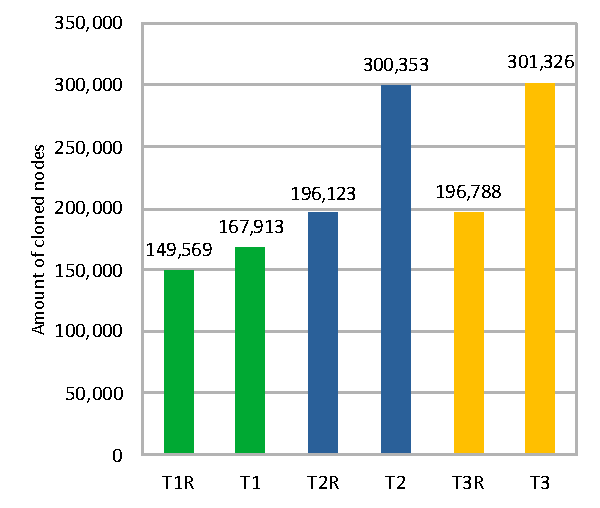
\includegraphics[width=.5\columnwidth]{img/TypeResults}
      \caption{Number of cloned declarations/statements.}
  \label{fig:typeres}
\end{figure}

In this figure, the number of cloned nodes per clone type are displayed. The difference between T1R and T1 is small (10.9\%), because most often textually equal code is also functionally equal. The difference between T2R and T2 is bigger (34.7\%) because the T2R definition is more strict. T3R and T3 are similar to T2R and T2 because our dataset does not have so many gapped clones for the thresholds used.

We also measured the duration of finding clones by the different clone types. Figure~\ref{fig:performance} shows the duration of detecting all clones in the corpus using CloneRefactor for different clone types. Although this data is partly dependent on our implementation of the clone types, there is a notable difference between the refactoring-oriented clone types and the literature clone types. The reason for this is further explained in Section~\ref{chap:challenge}.

\begin{figure}[H]
  \centering
    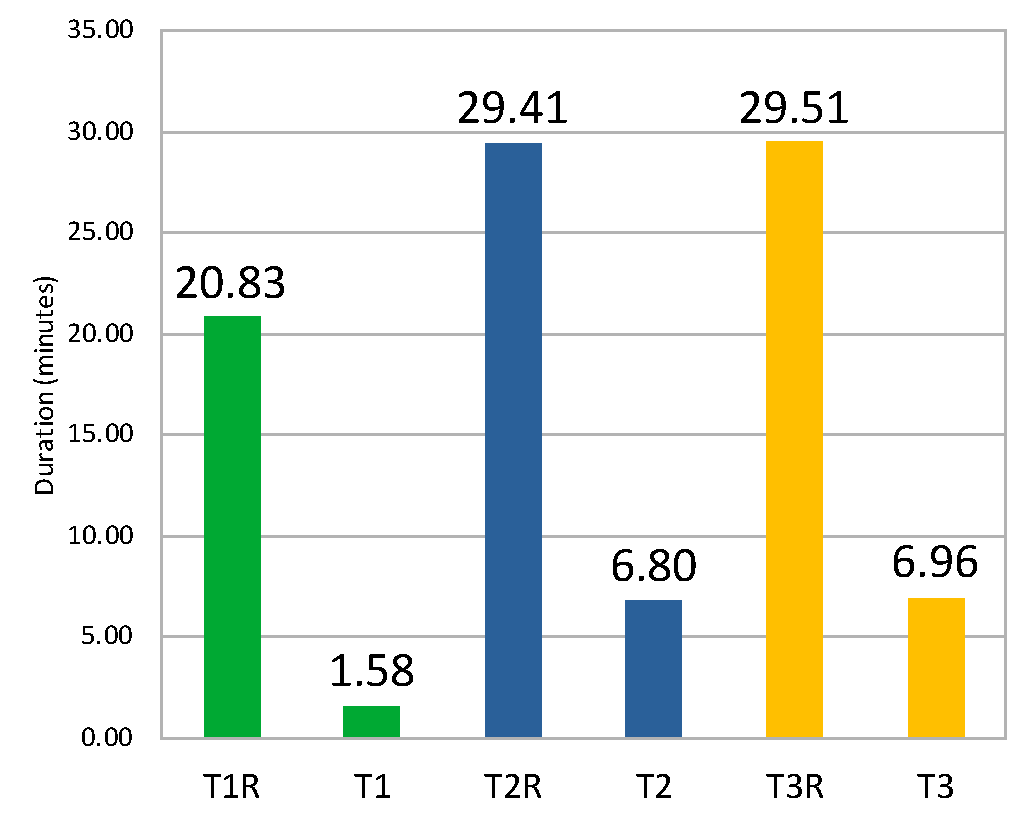
\includegraphics[width=.5\columnwidth]{img/DurationChart}
    \caption{Duration in minutes of identifying clones for clone type definitions.}
  \label{fig:performance}
\end{figure}

\subsection{Clone context}
% How many clones are there in certain contexts? Experiments for relation, location, and context.
To determine the refactoring method(s) that can be used to refactor most clones, we perform statistical analysis on the context of clones (see Sec.~\ref{sec:context}).

\subsubsection{Relation}
Table~\ref{tab:relation} displays the number of clone classes found for the entire corpus for different relations (see Sec.~\ref{sec:relation}).

\begin{table}[H]
\centering
\begin{tabular}{@{}llll@{}}
\toprule
\textit{\textbf{Category}} & \textit{\textbf{Relation}} & \textit{\textbf{Clone Classes}} & \textit{\textbf{Total}} \\ \midrule
\multirow{2}{*}{\begin{tabular}[c]{@{}l@{}}Common\\ Class\end{tabular}} & Same Class & 22,893 & \multirow{2}{*}{31,848} \\ \cmidrule(lr){2-3}
 & Same Method & 8,955 &  \\ \midrule
\multirow{5}{*}{\begin{tabular}[c]{@{}l@{}}Common\\ Hierarchy\end{tabular}} & Sibling & 15,588 & \multirow{5}{*}{20,342} \\ \cmidrule(lr){2-3}
 & Superclass & 2,616 &  \\ \cmidrule(lr){2-3}
 & First Cousin & 1,219 &  \\ \cmidrule(lr){2-3}
 & Common Hierarchy & 720 &  \\ \cmidrule(lr){2-3}
 & Ancestor & 199 &  \\ \midrule
\multirow{4}{*}{Unrelated} & No Direct Superclass & 10,677 & \multirow{4}{*}{20,314} \\ \cmidrule(lr){2-3}
 & External Superclass & 4,525 &  \\ \cmidrule(lr){2-3}
 & External Ancestor & 3,347 &  \\ \cmidrule(lr){2-3}
 & No Indirect Superclass & 1,765 &  \\ \midrule
\multirow{2}{*}{\begin{tabular}[c]{@{}l@{}}Common\\ Interface\end{tabular}} & Same Direct Interface & 7,522 & \multirow{2}{*}{13,074} \\ \cmidrule(lr){2-3}
 & Same Indirect Interface & 5,552 &  \\ \bottomrule
\end{tabular}
\caption{Number of clone classes per clone relation}
\label{tab:relation}
\end{table}

\subsubsection{Contents}
Table~\ref{tab:contents} displays the number of clone classes found for the entire corpus for different contents (see Sec.~\ref{sec:contents}).

\begin{table}[H]
\centering
\begin{tabular}{@{}llll@{}}
\toprule
\textit{\textbf{Category}} & \textit{\textbf{Contents}} & \textit{\textbf{Clone instances}} & \textit{\textbf{Total}} \\ \midrule
\multirow{2}{*}{Partial} & Partial Method & 219,540 & \multirow{2}{*}{229,521} \\ \cmidrule(lr){2-3}
 & Partial Constructor & 9,981 &  \\ \midrule
\multirow{5}{*}{Full} & Full Method & 12,990 & \multirow{5}{*}{13,173} \\ \cmidrule(lr){2-3}
 & Full Interface & 64 &  \\ \cmidrule(lr){2-3}
 & Full Constructor & 58 &  \\ \cmidrule(lr){2-3}
 & Full Class & 37 &  \\ \cmidrule(lr){2-3}
 & Full Enum & 24 &  \\ \midrule
\multirow{3}{*}{Other} & Several Methods & 22,749 & \multirow{3}{*}{53,773} \\ \cmidrule(lr){2-3}
 & Only Fields & 17,700 &  \\ \cmidrule(lr){2-3}
 & Other & 13,324 &  \\ \bottomrule
\end{tabular}
\caption{Number of clone instances for clone contents categories}
\label{tab:contents}
\end{table}

\subsection{Extract Method}
%To what extent can found clones be refactored through method extraction, without requiring additional transformations.
Table~\ref{tab:refactorability} shows to what extent clone classes can be refactored by using the ``Extract Method'' refactoring technique. The second column shows our measurements for the complete systems (just like the former experiments). The third column shows our measurements when restricting our search to method bodies. The amount that can be extracted increases because, when restricting our search to method bodies, we do not exclude declarations that can obstruct the possibility of method extraction (for instance a cloned method signature).

\begin{table}[H]
\centering
\begin{tabular}{@{}lll@{}}
\toprule
\textit{\textbf{Category}} & \textit{\textbf{All}} & \textit{\textbf{Method Body}} \\ \midrule
Can Be Extracted & 24,157 & 26,109 \\
Is Not A Partial Method & 21,625 & 0 \\
Top-level AST-Node is not a Statement & 19,887 & 4,607 \\
Spans Part of a Block & 12,964 & 13,460 \\
Multiple Return Values & 5,622 & 6,131 \\
Complex Control Flow & 1,106 & 1,216 \\ \bottomrule
\end{tabular}
\caption{Number of clones that can be extracted using the ``Extract Method'' refactoring technique}
\label{tab:refactorability}
\end{table}

\subsection{Refactoring}
%I think the ultimate goal with this thesis is to do experiments with different clone thresholds. Which thresholds give clones that we should refactor? For this, we will measure the maintainability of the refactored source code over different thresholds. These thresholds range from minimum clone size, variability, and gap size.
In our corpus, CloneRefactor has refactored 12.710 clone classes and measured the change in indicated metrics (see Sec.~\ref{sec:metrics}). Using the presented formulas (see Sec.~\ref{sec:metricformula}) we determine how the characteristics of the extracted method (see Sec.~\ref{sec:characteristics}) influence the maintainability of the resulting codebase after refactoring. In this section, we explore the data received by comparing the before- and after snapshots of the system for each separate refactoring.

\subsubsection{Clone Token Volume}
Figure \ref{fig:duplication} shows the obtained results when plotting the clone size (in tokens) vs the maintainability increase/decrease. On the secondary axis the amount of refactorings that have refactored a clone with the specified amount of tokens is displayed (e.g. the amount of data points the data is based on). As the amount of data points decreases, the datapoints gain less statistical significance.

\begin{figure*}
  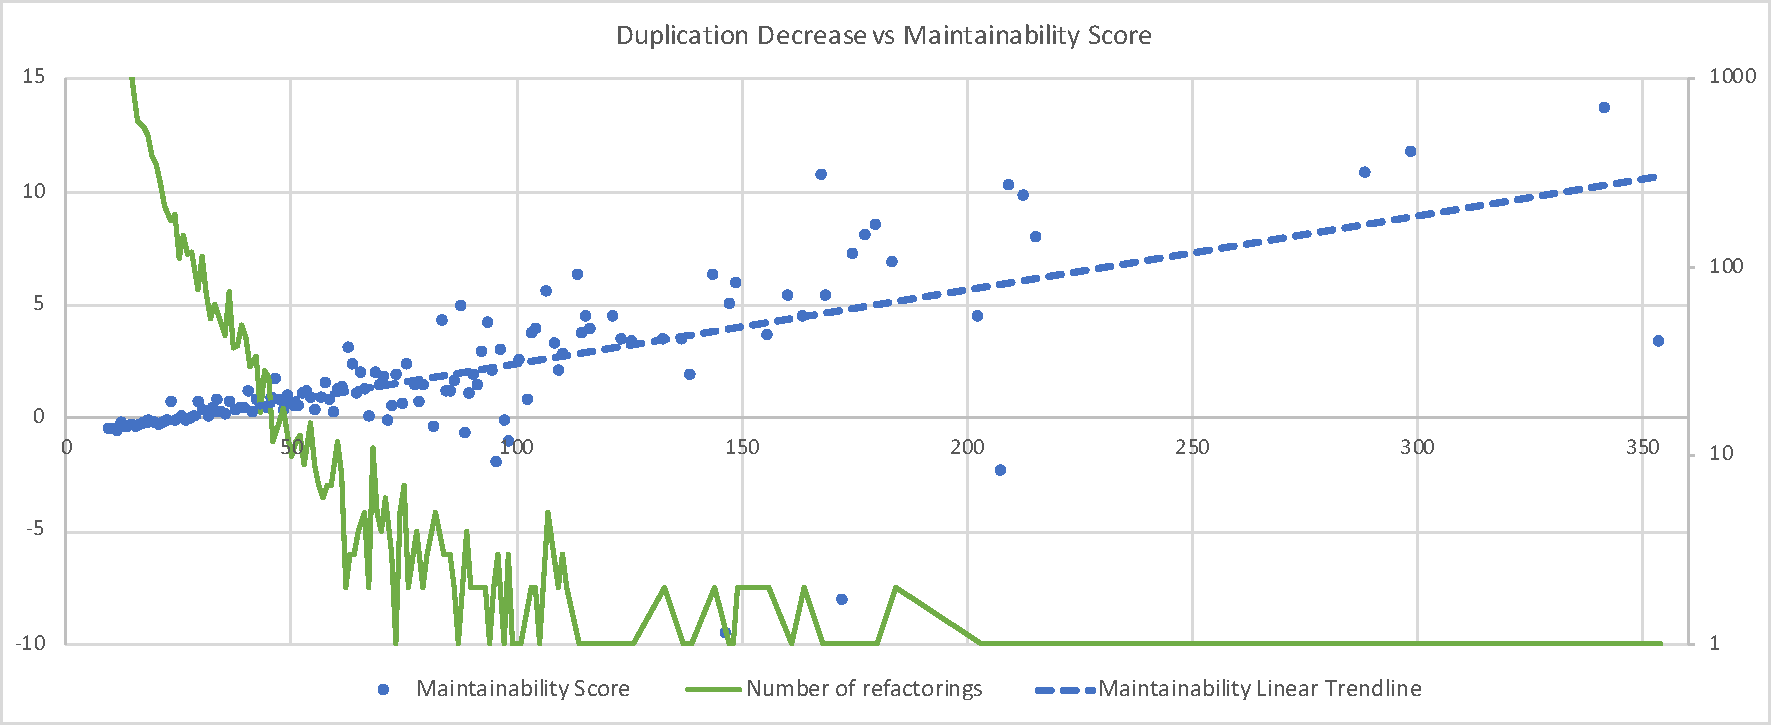
\includegraphics[width=1\textwidth]{img/duplication}
  \caption{A graph that shows how the size in tokens of the refactored clone affects maintainability. Maintainability on the primary axis and amount of refactorings on the secondary axis.}
  \label{fig:duplication}
\end{figure*}

The volume of the clone is the dominating factor regarding the maintainability increase/decrease of cloned code. Because of that, for our further experiments, we filter out all refactorings with a token size smaller than 18 because otherwise the small clones dominate the results and turn all results towards unmaintainable.

\subsubsection{Relation}
Table~\ref{tab:relation_refactor} shows our data regarding how different relations influence maintainability. We have marked rows based on less than 100 refactorings red, as their result does not have statistical significance.

\begin{table}[]
\centering
\begin{tabular}{@{}lll@{}}
\toprule
\textit{\textbf{Relation}} & \textit{\textbf{\begin{tabular}[c]{@{}l@{}}Maintainability\\ Score\end{tabular}}} & \textit{\textbf{\begin{tabular}[c]{@{}l@{}}Number of\\ Refactorings\end{tabular}}} \\ \midrule
\textbf{Common Hierarchy} & \textbf{0.51} & \textbf{792} \\ \midrule
\hspace{10pt} Sibling & 0.57 & 637 \\
\rowcolor[HTML]{FFCCC9}
\hspace{10pt} Same Hierarchy & 0.55 & 22 \\
\rowcolor[HTML]{FFCCC9}
\hspace{10pt} Superclass & 0.20 & 74 \\
\rowcolor[HTML]{FFCCC9}
\hspace{10pt} First Cousin & -0.02 & 53 \\
\rowcolor[HTML]{FFCCC9}
\hspace{10pt} Ancestor & -0.65 & 6 \\ \midrule
\textbf{Common Class} & \textbf{0.01} & \textbf{2,025}\\ \midrule
\hspace{10pt} Same Method & 0.01 & 762  \\
\hspace{10pt} Same Class & 0.01 & 1,263 \\ \midrule
\textbf{Unrelated} & \textbf{-0.02} & \textbf{688}\\ \midrule
\hspace{10pt} No Direct Superclass & 0.08 & 289 \\
\hspace{10pt} External Superclass & -0.02 & 225  \\
\rowcolor[HTML]{FFCCC9}
\hspace{10pt} No Indirect Superclass & -0.04 & 30  \\
\hspace{10pt} External Ancestor & -0.26 & 144  \\ \midrule
\textbf{Common Interface} & \textbf{-0.11} & \textbf{283} \\ \midrule
\hspace{10pt} Same Direct Interface & 0.02 & 160 \\
\hspace{10pt} Same Indirect Interface & -0.31 & 123
\end{tabular}
\caption{Influence on maintainability of refactoring clones by certain relations.}
\label{tab:relation_refactor}
\end{table}

\subsubsection{Return Value}
Table~\ref{tab:return} shows how the return value of the extracted method influences the maintainability of the resulting system.

\begin{table}[H]
\centering
\begin{tabular}{@{}lll@{}}
\toprule
\textit{\textbf{Return Value}} & \begin{tabular}[c]{@{}l@{}}\textit{\textbf{Maintainability}}\\\textit{\textbf{Score}}\end{tabular} & \begin{tabular}[c]{@{}l@{}}\textit{\textbf{Number of}}\\\textit{\textbf{Refactorings}}\end{tabular} \\ \midrule
Return & 0.20 & 421 \\
Void & 0.19 & 2052 \\
Declare & 0.03 & 1318 \\
\rowcolor[HTML]{FFCCC9}
Assign & -1.29 & 3 \\ \bottomrule
\end{tabular}
\caption{Maintainability scores for different return values}
\label{tab:return}
\end{table}

\subsubsection{Parameters}
Fig.~\ref{fig:arguments} shows how an increase in parameters lowers the maintainability of the refactored code. On the primary x-axis, the maintainability is displayed. The secondary x-axis shows the number of refactorings. The y-axis shows the number of parameters.

\begin{figure}[H]
  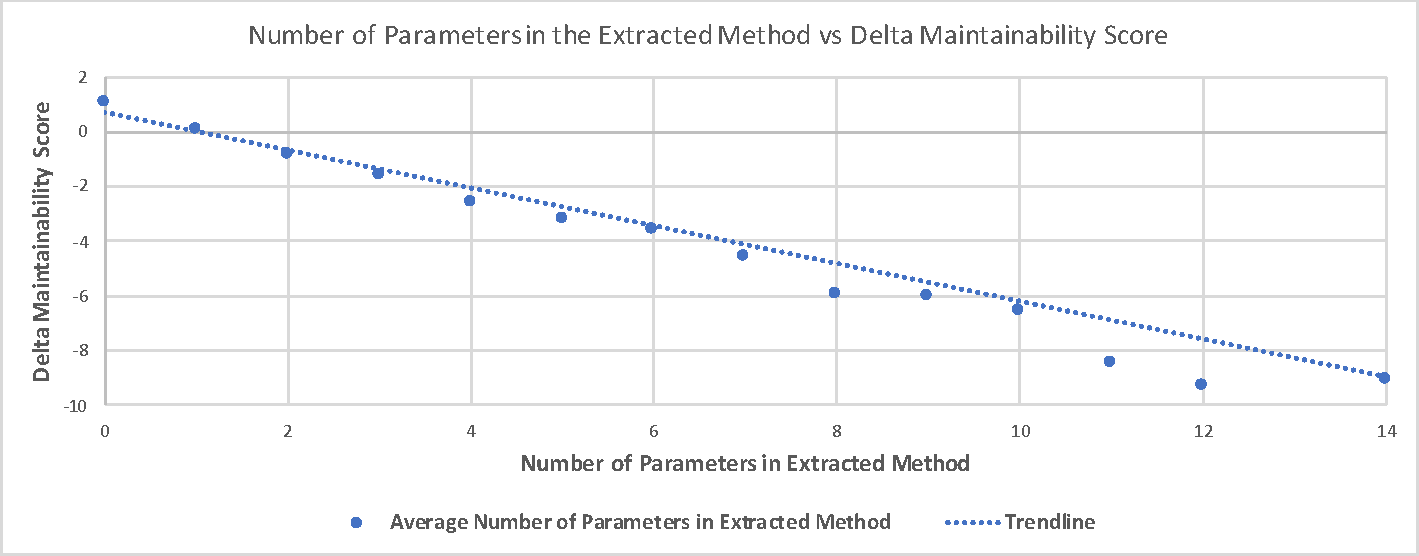
\includegraphics[width=1\columnwidth]{img/arguments}
  \caption{Influence of number of method parameters on system maintainability.}
  \label{fig:arguments}
\end{figure}

\section{Context Analysis of Clones}\label{chap:clonecontextexpl}
We analyzed the context of clones in a large corpus of open source projects. These experiments follow the structure of the context: The relation between clone instances is explained, measured and discussed in chapter \ref{chap:relationsinstances}; the location of clone instances is explained, measured and discussed in chapter \ref{chap:clonelocation};  he content of clone instances are explained, measured and discussed in chapter \ref{chap:clonecontents}.

\subsection{Relations Between Clone Instances} \label{chap:relationsinstances}
\todo{update these results}
In Section~\ref{sec:setuprelation} we introduced our experiments regarding relations between clones. Table~\ref{table:relations} contains our results regarding the relations between clone instances.

\begin{table}[H]
  \begin{center}
  \caption{Clone relations} \label{table:relations}
  \medskip
\begin{tabular}{|l|l|l|} \hline
\textbf{Relation} & \textbf{\#} & \textbf{\%} \\ \hline
Unrelated          & 12,368 & 34.88            \\ \hline
Same Class          & 11,483 & 32.38             \\ \hline
Same Method               & 5,056 & 14.26            \\ \hline
Sibling         & 4,182 & 11.79             \\ \hline
External Superclass   & 1,066 & 3.01             \\ \hline
Superclass          & 558 & 1.57           \\ \hline
First Cousin          & 489 & 1.38           \\ \hline
Common Hierarchy    & 206 & 0.58            \\ \hline
Ancestor          & 54 & 0.15          \\ \hline
\end{tabular}
\end{center}
\end{table}

The most notable difference when comparing it to the results of Fontana et al.~\cite{fontana2015duplicated} is that in our results most of the clones are unrelated (34.44\%), while for them it was only 15.70\%. This is likely due to the fact that we consider clone classes rather than clone pairs, and mark the clone class ``Unrelated'' even if just one of the clone instances is outside a hierarchy. It could also be that the corpus which we use, as it has generally smaller projects, uses more classes from outside the project (which are marked ``Unrelated'' if they do not have a common external superclass). About a third of all clone classes have all instances in the same class, which is generally easy to refactor. On the third place come the clones that are in the same method, which are similarly easy to refactor.

\subsection{Clone instance location}\label{chap:clonelocation}
\todo{update these results}
Measuring the clone locations categories defined in Section~\ref{sec:setuplocation} yields the results displayed in Table \ref{table:contents}.

\begin{table}[H]
  \begin{center}
  \caption{Clone instance locations} \label{table:locations}
  \medskip
\begin{tabular}{|l|l|l|}
\hline
\textbf{Location}   & \textbf{\#} & \textbf{\%} \\ \hline
Method Level        & 83,813 & 82.62            \\ \hline
Class Level        & 12,534 & 12.35            \\ \hline
Constructor Level    & 4,391 & 4.33           \\ \hline
Interface Level   & 567 & 0.56           \\ \hline
Enum Level         & 145 & 0.14            \\ \hline
\end{tabular}
\end{center}
\end{table}

Our results indicate that around 58\% of the clones are produced at method-level. About 39\% of clones either span several methods/constructors or contain something like a field declaration. Another 3\% of the clones are found in constructors. The amount of clones found in interfaces and enumerations is very low. Regarding the differences between type 1 and type 1R, it seems that there are relatively less method level clones and more class level clones for type 1R. This is probably due to that the main reason for variability between type 1 and type 1R is variable references, which occur more at method level than class level.

\subsection{Clone instance contents}\label{chap:clonecontents}
\todo{update these results}
Measuring the clone contents categories defined in Section~\ref{sec:setupcontents} yields the results displayed in Table \ref{table:contents}.

\begin{table}[H]
  \begin{center}
  \caption{Clone instance contents} \label{table:contents}
  \medskip
\begin{tabular}{|l|l|l|}
  \hline
  \textbf{Contents} & \textbf{\#} & \textbf{\%} \\ \hline
  Partial Method     & 79,945 & 78.80 \\ \hline
  Several Methods         & 7,323 & 7.22 \\ \hline
  Partial Constructor      & 4,385 & 4.32 \\ \hline
  Full Method           & 3,868 & 3.81 \\ \hline
  Only Fields           & 3,039 & 3.00 \\ \hline
  Includes Constructor  & 1,522 & 1.50 \\ \hline
  Includes Field        & 616 & 0.61 \\ \hline
  Includes Class Declaration  & 376 & 0.37 \\ \hline
  Other Categories    & 376 & 0.37\\ \hline
\end{tabular}
\end{center}
\end{table}

Unsurprisingly, most clones span a part of a method. The most used refactoring technique for clones that span part of a method is ``Extract Method''. Because of that, we focus our research efforts on refactoring such clones.

\section{Merging duplicate code through refactoring} \label{sec:refactorability}
\todo{update these results}
In Section~\ref{sec:refactorabilitysetup} we define categories regarding the extent to which clones can be refactored through method extraction. Our results are displayed in Table \ref{table:refactorability}.

\begin{table}[H]
  \begin{center}
  \caption{Refactorability through method extraction} \label{table:refactorability}
  \medskip
\begin{tabular}{|l|l|l|}
\hline
\textbf{}         & \textbf{\#} & \textbf{\%} \\ \hline
Can be extracted     & 14,664 & 41.35 \\ \hline
Spans part of a block  & 10,801 & 30.46 \\ \hline
Is not a partial method   & 8,074 & 22.77 \\ \hline
Complex control flow & 1,922 & 5.42 \\ \hline
\end{tabular}
\end{center}
\end{table}

From Table~\ref{table:refactorability}, we can see that 41\% of the clones can directly be refactored through method extraction (and possibly other refactoring techniques based on the relation of the clone instances). For the other clones, other techniques or transformations will be required.

\section{Refactoring clones}
\todo{TODO}

\chapter{Discussion}
\label{ch:discussion}
%Interpretations: what do the results mean?
%Implications: why do the results matter?
%Limitations: what can’t the results tell us?
%Recommendations: what practical actions or scientific studies should follow?

In this chapter, we discuss the results of our research and experiments.

\section{Clone Type Definitions}
In this study, we proposed a set of clone type definitions that can be automatically refactored.  We based these clone type definitions on the clone type definitions that are commonly used in literature. The design of these clone type definitions entails some decisions that have a large impact on the clones we considered for refactoring in this study. In this section we discuss our clone type definitions as proposed in Section~\ref{sec:rtypes}.

\subsection{Type 2R clones}
With type 2R clones we allow variability in some identifiers and literals such that the code can and should still be refactored. For type 2R clones we chose a set of expressions in which we allow variability and proposed a recommended refactoring strategy. We think however that type 2R could still use a lot of improvement to find more duplication patterns that can be refactored.

One method we think can be used to find more refactoring opportunities is to allow variability in expressions that have/return the same type. If expressions have/return the same type, they can be extracted to a parameter and the corresponding expression can be passed as a parameter. An example of this is displayed in Figure~\ref{fig:samereturn}. The only thing to watch out for is methods that have side effects. Because methods may be executed in another point during execution, this might affect the functionality of the code. Because of that, before applying such a refactoring it should be verified that the called method has to side effects.

\begin{figure}[H]
\begin{parcolumns}{2}
\colchunk[1]{
\begin{javacode}
// Original
public void doStuff(){
  int numbers = 456;
|\highlightYellow|  doA(getTitle());
|\highlightYellow|  doB(123);
  doC();
|\highlightYellow|  doA("456");
|\highlightYellow|  doB(numbers);
}

public String getTitle(){
  return "123";
}
\end{javacode}}
\colchunk[2]{
\begin{javacode}
// Refactored
public void doStuff(){
  int numbers = 456;
|\highlightYellow|  doAandB(getTitle(), 123);
  doC();
|\highlightYellow|  doAandB("456", numbers);
}

public void doAandB(String var1, int var2){
  doA(var1);
  doB(var2);
}

public String getTitle(){
  return "123";
}
\end{javacode}}
\end{parcolumns}
\caption{Refactoring different expressions that have the same return type.}
\label{fig:samereturn}
\end{figure}

\section{Clone Context Analysis}
In Section~\ref{chap:contextsetup} we introduced the categories we defined for mapping the context of clones. In this section, we discuss this together with the related experiments.

\section{CloneRefactor}
In this section we discuss our decisions for the design of our CloneRefactor tool.

\subsection{Clone Detection}
For CloneRefactor we chose to design a novel method of detecting clones, rather than using an existing clone detection technique or tool. Our rationale is as follows:
\begin{itemize}
  \item We perform comprehensive analysis on the source code which requires us to use an AST-based clone detection method.
  \item We perform dependency graph analysis, which requires us to resolve symbols in the source code.
  \item None of the existing clone detection methods implement all criteria required to build such a system.
\end{itemize}
By building a graph that maps relations between nodes in the AST, we can find clones in an efficient manner, allowing to perform a comprehensive analysis of large systems. This method has worked well for our purposes.

The main limitation we encountered is the memory required to build the clone graph. As we load the entire graph into memory before starting the clone detection procedure, this can cause issues on systems with low available memory. For a system consisting of 1.000.000 nodes, the clone graph requires about 4GB of RAM. For our corpus, there were no larger systems, so this was not a big issue. However, for industry projects our tool might require optimization.

\subsection{Context Analysis}
In this study we identified categories for three properties of clones: relation, location and contents. %Mapping the location and contents was mainly to find out what the best method of refactoring is to refactor most clones.
We chose a set of relations that indicate different refactoring opportunities. However, as our CloneRefactor tool only analyses Java source code, we we biased towards categories that are often found in Java source code. For other languages, other categories might be valuable to analyze to find suitable categories for that programming language.

\subsection{Refactoring}
In this section, we discuss our implementation decisions to refactor source code using CloneRefactor and measure its impact.

\subsubsection{Refactorability} \label{sec:discussrefactorability}
In Section~\ref{sec:refactorability} we introduced catagories to determine the refactorability of clones through method extraction. We excluded categories that could not not be directly refactored through method extraction. However, with a few transformations or further considerations it might be possible to make these clones refactorable. In this section we will highlight a few of these categories which we believe to be refactorable through method extraction with more effort.

\subsubsection{Partial block} \label{sec:partialblockdiscussion}
We did not consider clones for refactoring that span a part of a block. Although it is indeed not possible to refactor such clones, there are possibilities to make such clones refactorable. For instance, if the programming language supports lambda expressions, we can move the difference of statements in the block in a lambda expression \cite{tsantalis2017clone}. Figure \ref{fig:partialblockrefactoring} shows an example of such a refactoring opportunity.

\begin{figure}[H]
\begin{parcolumns}{2}
\colchunk[1]{
\begin{javacode}
// Original
public void doStuff(){
|\highlightYellow|  for(int i = 0; i<5; i++) { //Only the declaration of this for loop is cloned, but the loop body is not.
    System.out.println("hello!");
  }
|\highlightYellow|  for(int i = 0; i<5; i++) {
    CoreController.activateCore(i);
  }
}
\end{javacode}}
\colchunk[2]{
\begin{javacode}
// Refactored
public void doStuff(){
|\highlightYellow|  doFiveTimes(() -> System.out.println("hello!"));
|\highlightYellow|  doFiveTimes(() -> CoreController.activateCore(i));
}

public void doFiveTimes(Runnable runnable){
  for(int i = 0; i<5; i++) { //Only the declaration of this for loop is cloned, but the loop body is not.
    runnable.run();
  }
}
\end{javacode}}
\end{parcolumns}
\caption{Refactoring a method that is obstructed by a complex control flow.}
\label{fig:partialblockrefactoring}
\end{figure}

\subsubsection{Complex control flow}
Break, continue and return statements can obstruct the possibility of performing method extraction. However, with some extra transformations, method extraction will still be possible in such cases. Figure \ref{fig:complexcontrolflowrefactoring} shows such a transformation. We can wrap the newly extracted method in a conditional to indicate whether the ``control flow modifying statement'' should be executed. In other cases, other methods might apply to refactor such clones.

\begin{figure}[H]
\begin{parcolumns}{2}
\colchunk[1]{
\begin{javacode}
// Original
public boolean doStuff(){
|\highlightYellow|  if(doA());
|\highlightYellow|    return false;
|\highlightYellow|  doB();
  doC();
|\highlightYellow|  if(doA());
|\highlightYellow|    return false;
|\highlightYellow|  doB();
  return true;
}
\end{javacode}}
\colchunk[2]{
\begin{javacode}
// Refactored
public boolean doStuff(){
|\highlightYellow|  if(!doAandB())
|\highlightYellow|    return false;
  doC();
|\highlightYellow|  return doAandB();
}

public boolean doAandB(){
  if(doA())
    return false;
  doB();
  return true;
}
\end{javacode}}
\end{parcolumns}
\caption{Refactoring a method that is obstructed by a complex control flow.}
\label{fig:complexcontrolflowrefactoring}
\end{figure}

\subsubsection{Metrics}
For this study we chose to focus on a set of four metrics to measure maintainability: method size, duplication, method parameters and cyclomatic complexity. These metrics give an indication of the impact of the refactoring, but do not give a complete overview. There are many more metrics that could be considered to measure the maintainability impact on the system. An example of such a metric is ``coupling'', which focuses on the amount of incoming calls into a method or class and what modules these calls come from. This metric is also influenced by the transformations we applied and might deliver valuable insights in the quality of the refactoring.

In general, considering other metrics can result in a more reliable measure of the increase or decrease of maintainability after applying a specific refactoring.

\section{Results}
In this section, we discuss the results of our experiments.

\subsection{Clone Types}
In this section, we discuss the differences between clone types 1-3 and 1R-3R. We see that the difference between T1R and T1 in terms of found clones is small (11\%). This implies that most often textually equal code is also functionally equal. The difference between T2R and T2 is bigger (35\%). Upon manual inspection we found that the main reason for this is that T2R does not allow any variability in types, wheareas T2 allows any variability in types.

Regarding performance (Figure~\ref{fig:performance}, there is a notable difference between the refactoring-oriented clone types and the literature clone types. Type 1R-3R take about 6 times longer to detect than type 1-3. The main reason for this is type resolution: finding the fully qualified identifiers of type-, variable- and method-references.

In Figure~\ref{fig:t2rgraph} we show the increase of cloned nodes for a higher variability between clone instances. This graph is logaritmic: as the variability increases, the increase in nodes decreases. This implies that semantical equality increases the chances that tokens are equal.

In Figure~\ref{fig:t3rgraph} we show the increase of cloned nodes for higher type 3R gap sizes. The line denoting the number of clone classes seems a bit exponential whereas the line denoting cloned nodes is mostly linear. This makes sense regarding the nature of the threshold. As we get into higher gap size percentages, fewer clones merge (thus the decrease in amount of clone classes merging). However, at these higher gap size percentages the gaps contains more nodes (thus the amount of cloned nodes being linear).

\subsection{Clone Context}
Regarding clone context, our results indicate that most clones (37\%) are in a common class. This is favorable for refactoring because the extracted method does not have to be moved after extraction. 24\% of clones are in a common hierarchy. These refactorings are also often favorable. Another 24\% of clones are unrelated, which is often unfavorable because it often requires a more comprehensive refactoring. 15\% of clones are in an interface.

Regarding clone contents, 74\% of clones span part of a method body (77\% if we include constructors). 8\% of clones span several methods, which often require refactorings on a more architectural level. 6\% of clones span only global variables, requiring an abstraction to encapsulate these data declarations. Only 4\% of clones span a full declaration (method, class, constructor, etc.).

\subsection{Extract Method}
28\% of clones can be refactored using the ``Extract Method'' refactoring technique (50\% if we limit our searching scope to method bodies). About 25\% of clones do not span part of a method, because of which they cannot be refactored. Many clones (23\%) do not have a statement as top-level AST-Node. Upon manual inspection, we noticed that the main reason for this is clones in anonymous functions or anonymous classes. About 15\% of clones span only part of an AST-Node.

\subsection{Refactoring}
In Fig.~\ref{fig:maintainabilityscore} we see an increase in maintainability for refactoring larger clone classes. The tipping point, between a better maintainable refactoring and a worse maintainable refactoring, seems to lie at a token volume of 63 tokens. There are fewer large clones than small clones, resulting in a very limited statistical significance on our corpus when considering clones larger than 100 tokens.

In Table~\ref{tab:relationref} we see the results regarding refactorings that are applied to clones with diverse relations. We see that most refactored clones are in a common class, over 54\%. This is significantly more than the percentage of clones in the common class relation as reported in Table~\ref{tab:relation}. Meanwhile, the number of refactored unrelated clones is smaller than the number reported in Table~\ref{tab:relation} (24\% -> 18\%). The main reason for this is that refactoring unrelated clones can change the relation of other clones in the same system. If we create a superclass abstraction to refactor an unrelated clone, other clones in those classes that were previously unrelated might become related.

The maintainability scores displayed in Table~\ref{tab:relationref} show that the most favorable clones to refactor are clones with a sibling relation. The most unfavorable is to refactor clones to interfaces. However, the differences in maintainability in this table are generally small; according to our data relations have a minor impact on the maintainability of clones.

Regarding the return type of refactored clones, we see in Table~\ref{tab:return} that this has no major impact on maintainability. A method call to the extracted method that is directly returned and no return type extracted methods are slightly more favorable than the others. We think the main reason that the ``Return'' category is on top is that when a variable is declared at the end of the cloned fragment, CloneRefactor directly returns its value and removes the declaration. This decreases the volume slightly.

A higher number of parameters directly influences the corresponding metric. Because of this, we see in Fig.~\ref{fig:arguments} that more parameters negatively influence maintainability. Not only the number of parameters metric is negatively influenced, but more method parameters also increase volume for the extracted method and each of the calls to it. Because of that, we see that trend of the graph in Fig.~\ref{fig:arguments} decreases relatively rapidly.

\chapter{Conclusion}
\label{ch:conclusion}
In the research we have conducted so far we have made three novel contributions:
\begin{itemize}
    \item We proposed a method with which we can detect clones that can/should be refactored.
    \item We mapped the context of clones in a large corpus of open source systems.
    \item We mapped the opportunities to perform method extraction on clones this corpus.
\end{itemize}

We have looked into existing definitions for different types of clones \cite{roy2007survey} and proposed solutions for problems that these types have with regards to automated refactoring. We propose that fully qualified identifiers of method call signatures and type references should be considered instead of their plain text representation, to ensure refactorability. Furthermore, we propose that one should define thresholds for variability in variables, literals and method calls, in order to limit the number of parameters that the merged unit shall have.

The research that we have conducted so far analyzes the context of different kinds of clones and prioritizes their refactoring. Firstly, we looked at the inheritance relation of clone instances in a clone class. We have found that more than a third of all clone classes are flagged unrelated, which means that they have at least one instance that has no relation through inheritance with the other instances. For about a fourth of the clone classes all of its instances are in the same class. About a sixth of the clone classes have clone instances that are siblings of each other (share the same superclass).

Secondly, we looked at the location of clone instances. Most clone instances (58 percent) are found at method level. About 37 percent of clone instances were found at class level. We defined ``class level clones'' as clones that exceed the boundaries of a single method or contain something else in the class (like field declarations, other methods, etc.). Thirdly, we looked at the contents of clone instances. Most clones span a part of a method (57 percent). About 26 percent of clones span over several methods.

We also looked into the refactorability of clones that span a part of a method. Over 10 percent of the clones can directly be refactored by extracting them to a new method (and calling the method at all usages using their relation). The main reason that most clones that span a part of a method cannot directly be refactored by method extraction, is that they contain \texttt{return}, \texttt{break} or \texttt{continue} statements.

\section{Threats to validity}\label{chap:threatstovalidity}
We noticed that, when doing measurements on a corpus of this size, the thresholds that we use for the clone detection have a big impact on the results. There does not seem to be one golden set of thresholds, some thresholds work in some situations but fail in others. We have chosen thresholds that, according to our manual assessment, seemed optimal. However, by using these, we definitely miss some harmful clones.


\section{Future work} \label{sec:future_work}
This study presents a foundation for research in a largely unexplored field of studies: analyzing maintainability through automated refactoring. However, we scratched just the tip of the iceberg regarding all research opportunities in this field. In this section we describe possible extensions to this research, as well as other research opportunities in this field of studies.

\subsection{Automated Refactoring for more metrics}
In this study we presented evidence regarding the value of applying automated refactoring to analyze the before- and after state of source code and refactored source code. Analyzing these states we were able to analyze the improvement in maintainability after applying certain refactorings. This allows us to better assess thresholds by which maintainability issues in source code are identified. We also get better insights in the costs and values of applying certain refactoring efforts.

For this study we chose to focus only on the automated refactoring of duplication in source code. However, software maintainability depends on more factors and can be measured by more metrics. These factors also have opportunities to automate their refactorings. We think that several similarly sized studies can be conducted to automate the refactoring of other maintainability metrics.

A study by Heitlager et al. \cite{heitlager2007practical} presents several metrics by which the maintainability of source code can be assessed. They propose thresholds that indicate issues with these metrics. Many of these metrics have automated refactoring opportunities. In this section we will focus on several of these metrics to outline their opportunities for automated refactoring.

\subsubsection{Long parameter list}
When multiple parameters are used together in a method, there is an implicit dependency between these parameters: the dependency of being required by that method. If a lot of data hangs around really tight together, they should be made into their own object \cite{fowler1999refactoring, visser2016building}. Guidelines describe to limit the number of parameters per method to at most 4 \cite{visser2016building}.

If a method has many parameters, we can group strongly related parameters into an object. This can be done automatically, but two things must be considered:
\begin{itemize}
  \item How do we determine whether parameters are strongly related?
  \item At what other places is this data used in unison and should thus use the new abstraction?
\end{itemize}
To determine whether parameters are strongly related we must look into at what places they are used in the codebase. We must then define some threshold that denotes the percentage of usages of these variables in which they are used together. If this threshold exceeds a certain amount, we can group them into an object. We must then trace all places in which they are used together and replace the variables by the newly created abstractions.

\subsubsection{Method complexity}
Method complexity refers to the complexity of the logic in a method body. There are several methods to compute method complexity. The most used complexity metric is (MCCabe) Cyclomatic Complexity \cite{visser2016building}, which refers to the amount of independent paths that can be taken though the source code. Another complexity metric that has recently become fairly popular is Cognitive Complexity \cite{campbell2017cognitive}, which attempts to measure the human perceived complexity. Both indicate an aspect of source code maintainability.

Dealing with method complexity can largely be done by method extraction. We extract a part of a complex method to a new method. This way we split the complexity of the original method into separately testable methods. Also, the methods become easier to read.

Refactoring complex methods can largely be done automatically. Also, many of the results of this study can be reused. To assess an automated refactoring opportunity for complex methods, we should assess which parts of methods can be split to end up with parts of similar complexity. For this, our research can be used to assess whether a given piece of code can be extracted to a new method (see section \ref{sec:refactorability}).

We recommend to extend our tool, CloneRefactor, to allow for such capabilities. CloneRefactor already contains a component that calculates the Cyclomatic Complexity of a given method. Using our automated refactored model, identified problems can relatively easily be refactored.

\subsubsection{Method size}
Method size has a strong relation, in terms of refactoring, with Cyclomatic Complexity. Although method size is often related to Cyclomatic Complexity, a study by Landman et al. \cite{landman2016empirical} shows that Cyclomatic Complexity is not redundant to method size. However, they do share a similar method of refactoring. The automated refactoring opportunities described in the previous section also apply to method size.

\subsubsection{Combining the metrics}
Combining the automated refactoring models for each of these metrics can result in a model that ultimately provides significant improvement in the ease of writing well-maintainable source code. In this study, we presented a few tradeoffs that are the result of refactoring code clones. For instance, refactoring code clones with a lot of variability can result in long parameter lists. However, if we can combine this with automated refactoring of long parameter lists, this tradeoff can be mitigated. This way, it is possible to work towards an model of automated refactoring that reduces manual refactoring efforts significantly.

When programming, there are often trade-offs between technical debt and velocity. When a deadline comes near, often software quality in sacrificed to gain velocity \cite{costello1984software, austin2001effects, shah2014global}. Apart from that, a low programmer aptitude can result in low quality code \ref{cheney1984effects}. This is because often forming appropriate abstractions requires time, effort and critical thinking. By introducing these abstractions automatically, this negative impact can (partly) be mitigated.
%When programming, many developers must take decisions between velocity
%Many programmers report frequent decisions in which they decide to take technical debt

\subsection{Identifying more types/definitions for clones}
In this study, we proposed a set of clone type definitions for which a refactoring opportunity is known. We based these clone type definitions on the clone type definitions that are commonly used in literature. The design of these clone type definitions entails some decisions that have a large impact on the clones we considered for refactoring in this study.

\subsubsection{Type 2R clones}
With type 2R clones we allow variability in some identifiers and literals such that the code can and should still be refactored. For type 2R clones we chose a set of expressions in which we allow variability and proposed a recommended refactoring strategy. We think however that type 2R could still use a lot of improvement to find more duplication patterns that can be refactored.

One method we think can be used to find more refactoring opportunities is to allow variability in expressions that have/return the same type. If expressions have/return the same type, they can be extracted to a parameter and the corresponding expression can be passed as a parameter. The only thing to watch out for is method that have side effects. Because methods may be executed in another point during execution, this might affect the functionality of the code.
%TODO: Might want to show an example here

\subsubsection{Type 4 clones}
In section \ref{chap:backgroundclonetypes} we introduced the clone types that are used in literature. Of these clone types, we considered type 1, 2 and 3 for refactoring. We chose not to consider type 4 clones because they appear far less in source code and are more difficult to detect and refactor. However, that does not mean that these clones should not be refactored.

We think that there are relevant research opportunities in refactoring type 4 clones. Type 4 clones are functionally equal pieces of code that are implemented through different implementations. Although functionally equal, type 4 clones might still differ in other aspects. For instance, for type 4 clones, one alternative might be easier to maintain. Also, they can differ (significantly) in performance.

There are interesting research opportunities in automatically choosing the better alternative among type 4 clone instances.

\subsubsection{Proposing new clone type definitions}
We think that current definitions of clone types still lack in the identification of all duplication issues that a developer should invest his/her refactoring efforts in. Current clone detection techniques still result in many false positives and false negatives. By proposing good definitions for code clones that mark the characteristics of harmful anti-patterns, we can create more accurate suggestions to developers.

\subsection{Refactoring the harder to refactor clones}

\subsection{Naming of refactored methods/classes/etc.}
In this study, we took naming of refactored entities out of the scope. We applied automated refactoring to duplication, and gave all generated methods, classes and interfaces generated names. For our purposes that was not much of an issue, because of the validation methods used. We validated our approach using the SIG Maintainability model, which does not take naming quality into account. Because of that, the results of our experiments are in no way dependent on the names we give the generated methods, classes and interfaces.

When using our work with the purpose of refactoring assistance, these names will have to be manually provided. However, recent studies allow assistance in this process by generating a name that matches the body of a declaration. If this can be done in a reliable way, we can apply refactorings without any manual steps required.

A study by Allamanis et al. \cite{allamanis2015suggesting} proposes a machine learning model that can suggest accurate method and class names. This study shows promising results towards generating method and class names on basis of their body and context. However, the source code of this study in not available, making it harder to apply their findings to generate class and method names for any software project.

In a recent study by Alon et al. \cite{alon2018code2seq} they propose code2seq. Code2seq is a machine learning model that guesses the name of a method given a method body. This model has been trained on a large set of method bodies and names. The model already shows promising results. The source code of code2seq is publicly available, making it possible to embed this model in any application. Although this model is still far from perfect, combining it with our research could already greatly reduce the manual refactoring effort required. The main deficiency of this model lies in that its limited to the directly avail

\subsection{Looking into other languages/paradigms}
In this study we describe duplicate code refactoring opportunities for object-oriented languages. We built a tool to refactor code clones in Java and used it to run our experiments.

Applying our experiments with other programming languages than just Java might result in valuable results. Refactoring opportunities are greatly dependent on coding conventions, which differ per language. Other languages might result in different results, which might result in different insights regarding the resolution of duplication problems found. We prioritized refactoring efforts based on Java, which might differ from the prioritization that can result from running our experiments with other programming languages.

In this study we focused only on the object-oriented paradigm because of the shared concepts. However, the problems that come with duplication in source code also appears in different programming languages. Because of that, more insights could be obtained when looking into automated refactoring opportunities for other paradigms. For instance, it might be valuable to look into the opportunities to reduce duplication in the functional domain. Dealing with code clones in the functional paradigm is pretty much an unexplored field and might hold valuable results.

\subsection{Running our experiments with a greater diversity of software projects}
Currently

\subsection{Automatically refactoring code that is duplicated with a library}

\chapter*{Acknowledgements}
Throughout the writing of this dissertation, I have received a great deal of support and assistance. I would first like to thank my supervisor, Dr. A.M. Oprescu , whose expertise was invaluable in the academic writing and mathematical aspects of this thesis. Thank you for helping me concisely deliver the message I try to deliver.

Next, we would like to thank my peer student Sander Meester for always being there when I was stuck. Whenever I needed to test some ideas, you would always provide valuable insights. Your proofreading efforts helped me a lot to write this thesis.

I would like to thank my supervisor, Xander Schrijen, for all his input during our weekly meetings. We had long discussions about all my ideas, which helped to put my ideas in perspective.

I would like to thank Danny van Bruggen for all his help in my use of JavaParser. I am amazed by his willingness to help others to tackle their problems. JavaParser is at the core of the CloneRefactor tool and without Danny, I would never have come as far in the development of this tool.

Finally, I would like to acknowledge my colleagues from my internship at SIG for their wonderful collaboration. You supported me greatly and were always willing to help me.


\printbibliography[heading=bibintoc]
\printglossaries

\begin{appendices}

	\chapter{Refactoring maintainability metrics tables}

	\section{Token size}
\begin{longtable}[c]{@{}lllllll@{}}
\toprule
\textit{\textbf{Tokens}} & \textit{\textbf{\#}} & \textit{\textbf{Duplication}} & \textit{\textbf{Complexity}} & \textit{\textbf{Parameters}} & \textit{\textbf{Volume}} & \textit{\textbf{Score}} \\* \midrule
\endfirsthead
%
\multicolumn{7}{c}%
{{\bfseries Table \thetable\ continued from previous page}} \\
\toprule
\textit{\textbf{Tokens}} & \textit{\textbf{\#}} & \textit{\textbf{Duplication}} & \textit{\textbf{Complexity}} & \textit{\textbf{Parameters}} & \textit{\textbf{Volume}} & \textit{\textbf{Score}} \\* \midrule
\endhead
%
\bottomrule
\endfoot
%
\endlastfoot
%
10 & 1,273 & -31 & 1 & 1 & 12 & -0.08 \\
11 & 1,588 & -36 & 1 & 1 & 9 & -0.15 \\
12 & 1,390 & -37 & 1 & 1 & 12 & -0.30 \\
13 & 1,286 & -45 & 1 & 1 & 3 & 0.04 \\
14 & 1,345 & -43 & 1 & 1 & 9 & 0.01 \\
15 & 859 & -45 & 1 & 1 & 6 & -0.02 \\
16 & 596 & -50 & 1 & 1 & 4 & -0.25 \\
17 & 558 & -51 & 1 & 1 & 1 & -0.07 \\
18 & 484 & -65 & 1 & 1 & -2 & 0.13 \\
19 & 392 & -59 & 1 & 1 & -4 & 0.16 \\
20 & 348 & -52 & 1 & 1 & 4 & -0.13 \\
21 & 297 & -57 & 1 & 1 & -1 & -0.03 \\
22 & 195 & -59 & 1 & 1 & -4 & 0.00 \\
23 & 167 & -60 & 1 & 1 & -2 & 0.05 \\
24 & 206 & -93 & 0 & 1 & -29 & 1.27 \\
25 & 112 & -71 & 1 & 1 & -7 & -0.03 \\
26 & 152 & -70 & 1 & 1 & -11 & 0.06 \\
27 & 131 & -72 & 1 & 2 & -11 & 0.01 \\
28 & 114 & -66 & 1 & 2 & -6 & -0.18 \\
29 & 92 & -87 & 1 & 2 & -20 & 0.18 \\
30 & 110 & -131 & 1 & 2 & -47 & 0.96 \\
31 & 64 & -90 & 1 & 2 & -20 & 0.22 \\
32 & 59 & -85 & 1 & 2 & -13 & 0.07 \\
33 & 57 & -85 & 0 & 2 & -19 & 0.16 \\
34 & 53 & -92 & 0 & 2 & -18 & 0.33 \\
35 & 47 & -86 & 0 & 2 & -14 & 0.30 \\
36 & 66 & -89 & 1 & 1 & -13 & 0.32 \\
37 & 33 & -133 & 1 & 1 & -57 & 1.28 \\
38 & 40 & -92 & 1 & 1,825 & -17 & 0.06 \\
39 & 50 & -101 & 1 & 2 & -24 & 0.11 \\
40 & 43 & -113 & 0 & 2 & -30 & 0.54 \\
41 & 34 & -128 & -1 & 2 & -44 & 1.32 \\
42 & 34 & -104 & 1 & 2 & -22 & -0.19 \\
43 & 17 & -114 & -1 & 2 & -35 & 1.14 \\
44 & 23 & -101 & 0 & 1 & -27 & 0.76 \\
45 & 27 & -103 & 0 & 2 & -21 & 0.24 \\
46 & 13 & -110 & 0 & 2 & -20 & 0.45 \\
47 & 12 & -106 & 1 & 3 & -22 & -0.61 \\
48 & 21 & -110 & 0 & 2 & -27 & 0.69 \\
49 & 16 & -107 & 0 & 2 & -24,625 & 0.24 \\
50 & 6 & -100 & 1 & 2 & -16 & 0.30 \\
51 & 9 & -108 & 0 & 2 & -17 & 0.02 \\
52 & 13 & -104 & 1 & 1 & -14 & 0.38 \\
53 & 10 & -154 & 0 & 2 & -51 & 0.96 \\
54 & 16 & -158,625 & 875 & 2 & -56 & 0.45 \\
55 & 9 & -122 & 0 & 2 & -27 & 0.86 \\
56 & 6 & -131 & 0 & 3 & -22 & -0.56 \\
57 & 8 & -121,125 & 125 & 1,625 & -19 & 0.72 \\
58 & 6 & -203 & 1 & 3 & -82 & 0.83 \\
59 & 5 & -118 & 1 & 2 & -27 & 0.52 \\
60 & 10 & -126 & 0 & 3 & -18 & -0.77 \\
61 & 5 & -134 & 0 & 2 & -33 & 0.44 \\
62 & 3 & -124 & 1 & 1 & -36 & 1.51 \\
63 & 3 & -231 & -2 & 2 & -122 & 4.02 \\
64 & 3 & -213 & -2 & 3 & -91 & 2.02 \\
65 & 5 & -130 & 1 & 1 & -28 & 1.14 \\
66 & 4 & -165 & -1 & 2 & -64 & 1.90 \\
67 & 4 & -134 & 1 & 2 & -38 & 0.57 \\
68 & 10 & -143 & 1 & 4 & -25 & -1.81 \\
69 & 4 & -138 & 0 & 2 & -25 & 0.66 \\
70 & 4 & -228 & 1 & 2 & -104 & 2.78 \\
71 & 6 & -154 & 1 & 2 & -56 & 1.47 \\
72 & 5 & -144 & 1 & 3 & -34 & -0.29 \\
73 & 3 & -146 & 0 & 2 & -34 & 0.68 \\
74 & 7 & -180 & 1 & 1 & -65 & 1.94 \\
75 & 8 & -196,875 & 0 & 5 & -58,625 & -0.86 \\
76 & 3 & -152 & 1 & 1 & -40 & 1.33 \\
78 & 4 & -156 & 0 & 3 & -39 & 0.41 \\
79 & 2 & -158 & -1 & 4 & -29 & -0.80 \\
80 & 3 & -160 & 0 & 2 & -45 & 0.66 \\
82 & 5 & -197 & 0 & 7 & -38 & -3.59 \\
84 & 2 & -252 & -5 & 2 & -137 & 5.92 \\
85 & 3 & -170 & 1 & 3 & -46 & 0.15 \\
86 & 2 & -172 & 1 & 3 & -35 & 0.39 \\
87 & 1 & -174 & 1 & 2 & -51 & 0.89 \\
88 & 5 & -176 & -1 & 2 & -46 & 2.11 \\
89 & 3 & -178 & 1 & 8 & -15 & -4.98 \\
90 & 1 & -180 & 1 & 5 & -43 & -2.04 \\
91 & 2 & -182 & 0 & 3 & -49 & 0.90 \\
92 & 1 & -184 & 1 & 2 & -66 & 1.18 \\
93 & 2 & -186 & 1 & 1 & -73 & 2.46 \\
94 & 1 & -282 & 1 & 0 & -157 & 5.19 \\
95 & 1 & -190 & 1 & 1 & -67 & 2.20 \\
96 & 2 & -192 & 1 & 12 & 7 & -9.29 \\
97 & 1 & -291 & -1 & 5 & -132 & 1.06 \\
98 & 3 & -196 & 1 & 6 & -40 & -2.57 \\
99 & 1 & -198 & -1 & 8 & -6 & -4.34 \\
101 & 1 & -202 & -1 & 2 & -38 & 1.86 \\
103 & 1 & -206 & 1 & 13 & 2 & -10.05 \\
104 & 2 & -260 & -1 & 2 & -103 & 3.26 \\
105 & 1 & -210 & -2 & 2 & -70 & 2.82 \\
107 & 5 & -364 & -5 & 2 & -184 & 6.61 \\
108 & 1 & -216 & 0 & 1 & -65 & 2.86 \\
109 & 2 & -218 & -1 & 3 & -72 & 1.98 \\
110 & 4 & -303 & 1 & 6 & -117 & -0.66 \\
111 & 1 & -222 & 1 & 3 & -78 & 0.72 \\
113 & 1 & -226 & 1 & 0 & -83 & 3.70 \\
114 & 1 & -798 & 1 & 2 & -618 & 14.12 \\
115 & 1 & -230 & 1 & 1 & -96 & 2.95 \\
116 & 1 & -232 & -1 & 1 & -86 & 3.73 \\
117 & 1 & -1,053 & 1 & 15 & -572 & 3.38 \\
118 & 1 & -236 & 0 & 2 & -79 & 2.27 \\
124 & 1 & -248 & 1 & 2 & -98 & 2.18 \\
126 & 1 & -252 & 1 & 2 & -93 & 2.15 \\
133 & 3 & -266 & 1 & 2 & -80 & 1.93 \\
137 & 1 & -274 & 1 & 3 & -104 & 1.54 \\
139 & 1 & -278 & 1 & 5 & -77 & -0.70 \\
142 & 1 & -568 & -5 & 1 & -377 & 12.47 \\
144 & 2 & -288 & -3 & 2 & -108 & 4.95 \\
145 & 1 & -290 & 1 & 5 & -72 & -0.65 \\
147 & 1 & -294 & 1 & 21 & 96 & -18.17 \\
148 & 1 & -296 & 1 & 1 & -123 & 3.91 \\
149 & 2 & -298 & -3 & 2 & -108 & 4.34 \\
156 & 1 & -312 & 1 & 1 & -137 & 4.24 \\
161 & 1 & -322 & 1 & 1 & -127 & 4.20 \\
164 & 2 & -328 & -3 & 6 & -100 & 1.16 \\
168 & 1 & -336 & -10 & 2 & -137 & 8.45 \\
169 & 1 & -338 & 1 & 2 & -137 & 3.52 \\
173 & 1 & -346 & 1 & 23 & 25 & -18.66 \\
175 & 1 & -350 & -4 & 3 & -128 & 4.80 \\
180 & 1 & -360 & -5 & 2 & -139 & 6.44 \\
184 & 2 & -368 & -2 & 3 & -137 & 4.66 \\
203 & 1 & -406 & 1 & 6 & -148 & 0.46 \\
208 & 1 & -624 & 1 & 28 & -138 & -18.75 \\
210 & 1 & -420 & -5 & 2 & -184 & 7.59 \\
213 & 1 & -639 & 1 & 2 & -391 & 9.64 \\
216 & 1 & -432 & 1 & 1 & -189 & 6.02 \\
289 & 1 & -578 & 1 & 2 & -263 & 7.37 \\
299 & 1 & -598 & 1 & 1 & -272 & 8.63 \\
342 & 1 & -684 & 1 & 1 & -317 & 10.01 \\
354 & 1 & -708 & 1 & 18 & -202 & -7.57 \\* \midrule
\textbf{Total} & \textbf{12,683} & \textbf{-53.26} & \textbf{0.84} & \textbf{1.12} & \textbf{1.33} & \textbf{0.00} \\* \bottomrule
\caption{Refactored clones grouped by clone instance size in tokens}
\label{tab:full_token_refactoring}\\
\end{longtable}
\todo{Need to think about what to put here. I have a lot of stuff I'd like to put here, however my datasets are rather large. For one, I'd like to put my list of used systems here. However, it has 2267 items. I would like to put the refactorings here. However, it has 12684 items. I'd like to share more CloneRefactor output and stuff. However, it is rather much.}

\todo{Appendix: definitely share some tables in which the metrics are still separated and not yet aggregated. If the aggregation is wrong, we at least have the separated numbers.}

\end{appendices}


%comment out in the final version
%\listoftodos[Notes]

\end{document}
